%%%%%%%%%%%%%%%%%%%%%%%%%%%%%%%%%%%%%%%%%
% Oliver Lemon made minor edits (jan 2015)  to : 
% Masters/Doctoral Thesis 
% LaTeX Template
% Version 1.43 (17/5/14)
%
% This template has been downloaded from:
% http://www.LaTeXTemplates.com
%
% Original authors:
% Steven Gunn 
% http://users.ecs.soton.ac.uk/srg/softwaretools/document/templates/
% and
% Sunil Patel
% http://www.sunilpatel.co.uk/thesis-template/
%
% License:
% CC BY-NC-SA 3.0 (http://creativecommons.org/licenses/by-nc-sa/3.0/)
%
% Note:
% Make sure to edit document variables in the Thesis.cls file
%
%%%%%%%%%%%%%%%%%%%%%%%%%%%%%%%%%%%%%%%%%

%----------------------------------------------------------------------------------------
%	PACKAGES AND OTHER DOCUMENT CONFIGURATIONS
%----------------------------------------------------------------------------------------

\documentclass[11pt, oneside]{Thesis} % The default font size and one-sided printing (no margin offsets)

\graphicspath{{Pictures/}} % Specifies the directory where pictures are stored

\usepackage[square, comma, sort&compress]{natbib} % Use the natbib reference package - read up on this to edit the reference style; if you want text (e.g. Smith et al., 2012) for the in-text references (instead of numbers), remove 'numbers' 
\hypersetup{urlcolor=blue, colorlinks=true} % Colors hyperlinks in blue - change to black if annoying

\usepackage[labelfont=bf,textfont=md]{caption}

\title{Neural Models for Information Retrieval} % BUT you should use use " \title{\ttitle} " here instead to define the thesis title ! 
% \ttitle is defined in the file Thesis.cls 
% \sloppy
\begin{document}

\frontmatter % Use roman page numbering style (i, ii, iii, iv...) for the pre-content pages

\setstretch{1.3} % Line spacing of 1.3

% Define the page headers using the FancyHdr package and set up for one-sided printing
\fancyhead{} % Clears all page headers and footers
\rhead{\thepage} % Sets the right side header to show the page number
\lhead{} % Clears the left side page header

\pagestyle{fancy} % Finally, use the "fancy" page style to implement the FancyHdr headers

\newcommand{\HRule}{\rule{\linewidth}{0.5mm}} % New command to make the lines in the title page

% PDF meta-data
\hypersetup{pdftitle={\ttitle}}
\hypersetup{pdfsubject=\subjectname}
\hypersetup{pdfauthor=\authornames}
\hypersetup{pdfkeywords=\keywordnames}

%-----------------------------------------------------
%	TITLE PAGE
%-----------------------------------------------------

\begin{titlepage}
\begin{center}

\textsc{\LARGE \univname}\\[1.5cm] % University name
\textsc{\Large Masters Thesis}\\[0.5cm] % Thesis type

\HRule \\[0.4cm] % Horizontal line
{\huge \bfseries \ttitle}\\[0.4cm] % Thesis title
\HRule \\[1.5cm] % Horizontal line
 
\begin{minipage}{0.4\textwidth}
\begin{flushleft} \large
\emph{Author:}\\
\href{}{\authornames} % Author name - remove the \href bracket to remove the link
\end{flushleft}
\end{minipage}
\begin{minipage}{0.4\textwidth}
\begin{flushright} \large
\emph{Supervisors:} \\
\href{}{\supname} \\ % Supervisor name - remove the \href bracket to remove the link
M.Sc. Jaspreet Singh
\end{flushright}
\end{minipage}\\[1cm]
\begin{minipage}{0.8\textwidth}
\begin{flushright} \large
\emph{Examiners:} \\
\href{}{\supname} \\ % Supervisor name - remove the \href bracket to remove the link
\href{}{\examname}
\end{flushright}
\end{minipage}\\[2cm]
 
\large \textit{A thesis submitted in fulfillment of the requirements\\ for the degree of \degreename}\\[0.3cm] % University requirement text
\textit{in the}\\[0.4cm]
%\groupname\\

\deptname\\[2cm] % Research group name and department name
 
{\large \today}\\[1cm] % Date

\includegraphics[width=6cm]{./Figures/uni_hannover.png} % University/department logo - uncomment to place it
 
\vfill
\end{center}

\end{titlepage}

%-----------------------------------------------------
%	DECLARATION PAGE
%	Your institution may give you a different text to place here
%-----------------------------------------------------
\addtocontents{toc}{\vspace{-1em}}
\Declaration{

\addtocontents{toc}{} % Add a gap in the Contents, for aesthetics

I, \authornames, declare that this thesis titled, `\ttitle' and the work presented in it is my own. I confirm that this work submitted for assessment is my own and is
  expressed in my own words. Any uses made within it of the works of
  other authors in any form (e.g., ideas, equations, figures, text,
  tables, programs) are properly acknowledged at any point of their
  use. A list of the references employed is included.

%\begin{itemize} 
%\item[\tiny{$\blacksquare$}] This work was done wholly or mainly while in candidature for a research degree at this University.
%\item[\tiny{$\blacksquare$}] Where any part of this thesis has previously been submitted for a degree or any other qualification at %this University or any other institution, this has been clearly stated.
%\item[\tiny{$\blacksquare$}] Where I have consulted the published work of others, this is always clearly attributed.
%\item[\tiny{$\blacksquare$}] Where I have quoted from the work of others, the source is always given. With the exception of such %quotations, this thesis is entirely my own work.
%\item[\tiny{$\blacksquare$}] I have acknowledged all main sources of help.
%\item[\tiny{$\blacksquare$}] Where the thesis is based on work done by myself jointly with others, I have made clear exactly what %was done by others and what I have contributed myself.\\
%\end{itemize}
 \vspace{2cm} 
Signed:\\
\rule[1em]{25em}{0.5pt} % This prints a line for the signature
 
Date:\\
\rule[1em]{25em}{0.5pt} % This prints a line to write the date
}

\clearpage % Start a new page

%-----------------------------------------------------
%	QUOTATION PAGE
%-----------------------------------------------------

%\pagestyle{empty} % No headers or footers for the following pages

%\null\vfill % Add some space to move the quote down the page a bit

%\textit{``Thanks to my solid academic training, today I can write hundreds of words on virtually any topic without possessing a shred of information, which is how I got a good job in journalism."}

%\begin{flushright}
%Dave Barry
%\end{flushright}

%\vfill\vfill\vfill\vfill\vfill\vfill\null % Add some space at the bottom to position the quote just right

%\clearpage % Start a new page

%-----------------------------------------------------
%	ABSTRACT PAGE
%-----------------------------------------------------

\addtotoc{Abstract} % Add the "Abstract" page entry to the Contents

%\abstract{\addtocontents{toc}{\vspace{1em}} % Add a gap in the Contents, for aesthetics

 {\huge{\textit{Abstract}} \par}{\addtocontents{toc}{} 

In recent years, many deep neural network models have been proposed for the ad-hoc retrieval task. They have shown to perform better than traditional information retrieval baselines such as BM25, query-likelihood (QL) and some state-of-the-art learning-to-rank approaches that requires a lot of hand-crafted feature engineering. In this thesis, we first implement a  select few neural IR approaches (DRMM, MatchPyramid, PACRR-DRMM, NPRF-DRMM) using the standard TREC newswire collection (Robust04) to see how well we can reproduce the results highlighted in the respective papers.

In the second part of the thesis, we focus on the question--why a \textit{document} is relevant to a  query using a particular neural model. In the ML community, several approaches for explaining decisions made by deep neural networks have been proposed -- including DeepSHAP which modifies the DeepLift algorithm to estimate the relative importance (shapley values) of input features for a given decision by comparing the activations in the network for a given image against the activations caused by a reference input. In image classification, the reference input tends to be a plain black image. While DeepSHAP has been well studied for image classification tasks, we see how we can adapt it to explain the output of Neural Retrieval Models (NRMs). In particular, what is a good ``black'' image in the context of IR? In this thesis, we explored various reference input document construction techniques. Additionally, we compared the explanations generated by DeepSHAP to LIME (a model agnostic approach) and found that the explanations differ considerably. This study raises concerns regarding the robustness and accuracy of explanations produced for NRMs. With this work we aim to shed light on interesting problems surrounding interpretability in NRMs and highlight areas of future work.
%The page is kept centered vertically so can expand into the blank space above the title too\ldots
%

\clearpage % Start a new page

%-----------------------------------------------------
%	ACKNOWLEDGEMENTS
%-----------------------------------------------------

\setstretch{1.3} % Reset the line-spacing to 1.3 for body text (if it has changed)

\acknowledgements{\addtocontents{toc}{} % Add a gap in the Contents, for aesthetics

First, I would like to thank my supervisor Prof. Dr. Avishek Anand for giving me the opportunity to work on this interesting and challenging topic for my thesis and also for his constant guidance and invaluable ideas. I am also extremely grateful for his understanding and support in helping me change my topic mid-way through my thesis.

I would like to thank Jaspreet Singh for his invaluable suggestions that helped me successfully  train most of these neural ranking models and for always being available to talk through various approaches and ideas. 

I would also like to thank Prof. Dr. Wolfgang Nejdl for giving me the opportunity to work at L3S Research Center during my masters on a lot of interesting and diverse research problems ranging from Information Retrieval, Machine Learning to User Interface Design.

I would like to thank my friends for their constant support and help during this journey that had many ups and downs. 

Finally, I am grateful to my parents for supporting me in the decisions I made. I am deeply thankful for their constant source of encouragement and belief in me and also Cheryl, my wonderful and talented sister who picks my brain from time to time to understand the fundamentals of programming.
}
\clearpage % Start a new page

%-----------------------------------------------------
%	LIST OF CONTENTS/FIGURES/TABLES PAGES
%-----------------------------------------------------

\pagestyle{fancy} % The page style headers have been "empty" all this time, now use the "fancy" headers as defined before to bring them back

\lhead{\emph{Contents}} % Set the left side page header to "Contents"
\tableofcontents % Write out the Table of Contents


\lhead{\emph{List of Figures}} % Set the left side page header to "List of Figures"
\listoffigures % Write out the List of Figures

\lhead{\emph{List of Tables}} % Set the left side page header to "List of Tables"
\listoftables % Write out the List of Tables

%-----------------------------------------------------
%	ABBREVIATIONS
%-----------------------------------------------------

\clearpage % Start a new page

\setstretch{1.5} % Set the line spacing to 1.5, this makes the following tables easier to read

\lhead{\emph{Abbreviations}} % Set the left side page header to "Abbreviations"
\listofsymbols{ll} % Include a list of Abbreviations (a table of two columns)
{
\textbf{CBOW} & \textbf{C}ontinuous \textbf{B}ag  \textbf{O}f \textbf{W}ords \\
\textbf{CNN} & \textbf{C}onvolutional \textbf{N}eural \textbf{N}etwork \\
\textbf{DESM} & \textbf{D}ual \textbf{E}mbedding  \textbf{S}pace \textbf{M}odel \\
\textbf{DRMM} & \textbf{D}eep \textbf{R}elevance  \textbf{M}atching \textbf{M}odel \\
\textbf{DSSM} & \textbf{D}eep \textbf{S}tructured  \textbf{S}emantic \textbf{M}odel \\
\textbf{IR} & \textbf{I}nformation \textbf{R}etrieval\\
\textbf{LIME} & \textbf{L}ocal \textbf{I}nterpretable  \textbf{M}odel-agnostic \textbf{E}xplanations \\
\textbf{LM} & \textbf{L}anguage \textbf{M}odel \\
\textbf{LTR} & \textbf{L}earning-\textbf{T}o-\textbf{R}ank\\
\textbf{MLP} & \textbf{M}ulti-\textbf{L}ayer \textbf{P}erceptron\\
\textbf{NN} & \textbf{N}eural \textbf{N}etwork \\
\textbf{NPRF} & \textbf{N}euro \textbf{P}seudo  \textbf{R}elevance \textbf{F}eedback \\
\textbf{NRM} & \textbf{N}eural \textbf{R}etrieval \textbf{M}odel \\
\textbf{OOV} & \textbf{O}ut-\textbf{O}f-\textbf{V}ocabulary \\
\textbf{QL} & \textbf{Q}uery \textbf{L}ikelihood \\
\textbf{RNN} & \textbf{R}ecurrent \textbf{N}eural \textbf{N}etwork \\
}

%-----------------------------------------------------
%	PHYSICAL CONSTANTS/OTHER DEFINITIONS
%-----------------------------------------------------

%\clearpage % Start a new page

%\lhead{\emph{Physical Constants}} % Set the left side page header to "Physical Constants"

%\listofconstants{lrcl} % Include a list of Physical Constants (a four column table)
%{
%Speed of Light & $c$ & $=$ & $2.997\ 924\ 58\times10^{8}\ \mbox{ms}^{-\mbox{s}}$ (exact)\\

%% Constant Name & Symbol & = & Constant Value (with units) \\
%}

%-----------------------------------------------------
%	SYMBOLS
%-----------------------------------------------------

%\clearpage % Start a new page

%\lhead{\emph{Symbols}} % Set the left side page header to "Symbols"

%\listofnomenclature{lll} % Include a list of Symbols (a three column table)
%{
%$a$ & distance & m \\
%$P$ & power & W (Js$^{-1}$) \\
% Symbol & Name & Unit \\

%& & \\ % Gap to separate the Roman symbols from the Greek

%$\omega$ & angular frequency & rads$^{-1}$ \\
% Symbol & Name & Unit \\
%}

%-----------------------------------------------------
%	DEDICATION
%-----------------------------------------------------

%\setstretch{1.3} % Return the line spacing back to 1.3

%\pagestyle{empty} % Page style needs to be empty for this page

%\dedicatory{For/Dedicated to/To my\ldots} % Dedication text

%\addtocontents{toc}{\vspace{2em}} % Add a gap in the Contents, for aesthetics

%-----------------------------------------------------
%	THESIS CONTENT - CHAPTERS
%-----------------------------------------------------

\mainmatter % Begin numeric (1,2,3...) page numbering

\pagestyle{fancy} % Return the page headers back to the "fancy" style

% Include the chapters of the thesis as separate files from the Chapters folder
% Uncomment the lines as you write the chapters

% Chapter Template

\chapter{Introduction} % Main chapter title

\label{Chapter1} % Change X to a consecutive number; for referencing this chapter elsewhere, use \ref{ChapterX}

\lhead{Chapter 1. \emph{Introduction}} % Change X to a consecutive number; this is for the header on each page - perhaps a shortened title


In recent years, deep neural networks have achieved state of the art results in various tasks or domains, such as, computer vision, speech recognition and machine translation tasks~\citep{lecun2015deep}. These models have shown to be effective at learning abstract representations from the raw input (large training datasets), and the models have sufficient generalizability to be able to tackle different learning problems. These are desirable properties for the problem of relevance ranking in Information Retrieval (IR) and in recent years there have been a substantial number of works that applied these neural methods in IR displaying advances in state of the art.

Information retrieval is a core component in many real-world applications--Web search, digital libraries, e-commerce platforms and so on. The problem of relevance ranking in IR (\textit{ad-hoc} retrieval) is defined as--given a query and set of candidate documents, a scoring function determines the degree of relevance of the document to the query and finally produces a ranking list by sorting the relevance scores. Many different ranking models have been proposed including vector space models (TF-IDF), probabilistic retrieval models (BM25, QL) and learning to rank (LTR) approaches that applies machine learning to the ranking function achieving great improvements in retrieval effectiveness~\citep{liu2009learning}. However, successful LTR models relies heavily on hand-crafted feature engineering that is time-confusing, incomplete and over-specified. Thus, neural IR models that employ the use of shallow or deep neural networks for IR have been proposed as a solution to tackle the feature engineering problem of learning to rank, by using only automatically learned features from raw text input of the query and document. These neural IR models use vector representations of text, and have a large number of parameters that needs to be tuned with large-scale datasets in training~\citep{Mitra2017a}. Therefore, unlike traditional IR models, these models are more ``data-hungry'' and the performance increases as training data increases.

All existing neural IR can be broadly categorized based on whether they influence the query representation that encodes information need, or the document representation that captures distribution of information contained or estimate the mutual relevance based on patterns of matching between the query and document. They are categorized, as \textit{representation-based} approaches (DSSM~\citep{dssm13}, CDSSM~\citep{Shen2014a, Shen2014b}), and \textit{interaction-based} approaches (DRMM~\citep{Guo2016}, DUET~\citep{Mitra2017a}, MatchPyramid~\citep{matchpyramid16}, PACRR~\citep{pacrr17, co_pacrr_wsdm18}, K-NRM~\citep{KNRM17}). The representation-based approaches aimed to learn document representations to match with query representations, while interaction-based approaches learn from matching matrices between query and document. Recently, there have been works that focused on architectures that try to model the human relevance judgement process (DeepRank~\citep{Pang_deeprank_2017}) and on learning relevance signals at different granularities (i.e. passage-level or document-wide)~\citep{Fan_hint_2018}. The various neural ranking models learned from generating the features automatically have already outperformed several state-of-the-art LTR models with tens of hand crafted features~\citep{Pang_deeprank_2017, Fan_hint_2018}. There have been some interesting works whose focus has been on the training strategies of neural ranking models as not everyone has access to commercial large-scale training datasets~\citep{Dehghani_sigir17, dehghani2018fidelityweighted} and learning alternative indexing schemes for neural IR models~\citep{Zamani_neural_reranking_2018} that moves from the neural re-ranking strategies (\textit{telescoping}) adopted by most previous approaches.

With the spurt in performance of \textit{deep learning} in many domains, there has come a new wave of approaches trying to explain the decisions made by these complex machine learning models. Explainability and interpretability is at the heart of how one can  deploy NNs approaches in real-word applications and how humans will interact with them. These explanations can help debug models, determine training biases or understand decisions in simpler terms to build trust. With the recent progress of neural IR approaches that has shown state-of-the-art performance on certain benchmarks, the need to understand and analyze why these models are performing better or how they are connected to the classical IR approaches has become an important topic raised in the IR community~\citep{craswell2017sigir, Craswell2018sigir_forum}.

%------------------------------------------------------
%	SECTION 1
%------------------------------------------------------
\section{Motivation}
\textbf{Reproducibility} The rapid increase of new neural ranking models proposed in the literature, with each using different pre-processing strategies, different hyper-parameter choices, different benchmark datasets (public or large-scale private clickthrough data) and different scale of computational resources, highlights the issue of reproducibility and applicability of these new approaches. This has led to the focus of reproducibility of these methods that have been discussed in the IR community lately at relevant workshops~\citep{craswell2017sigir, Craswell2018sigir_forum} and also there has been the release of the large-scale dataset (MS-MARCO)~\citep{nguyen2016ms_marco} for the passage re-ranking task\footnote{\url{https://github.com/dfcf93/MSMARCO/blob/master/Ranking/README.md}} and TREC 2019 deep learning track\footnote{\url{https://trec.nist.gov/pubs/call2019.html}} for benchmarking emerging neural IR approaches.  

\textbf{Interpretability} The explainability of neural ranking models is largely unexplored. There have been few papers that focused on the interpretability of neural ranking models~\citep{Singh19} and on the diagnosis or analysis of different model components of the model empirically~\citep{PangLG0C17, Cohen18} or with the use of diagnostic datasets based on formal retrieval constraints~\citep{Rennings19}. It is interesting to see to what extent we can use the explainability approaches proposed in other domains (image or text classification) to understand the decisions of neural networks, which can be applied in the context of IR. Thus, its a challenging and promising direction of research in neural IR.

%------------------------------------------------------
%	SECTION 2
%------------------------------------------------------
\section{Contributions}

The work in this thesis can be divided into two parts--the first part focuses mainly on the reproducibility of various neural ranking models (both \textit{representation-based} and \textit{interaction-based}); and the second part focuses on the question--\textit{why} a particular document is relevant to a query for the various neural ranking models implemented part of the reproducibility experiments. 

We address the following questions in this thesis:
% \vspace{-1em}
\begin{itemize}
    \item What are the challenges in the reproducibility of the neural ranking models on the standard TREC Robust04 benchmark collection? Are we able to reproduce the same retrieval performance as mentioned in the papers? If not, why?\vspace{1em}
    \item How can we adapt the \textit{model-introspective} approach DeepSHAP to explain the output of neural ranking models?
    \item How different are the DeepSHAP explanations across the various implemented neural ranking models?
    \item How do the explanations from DeepSHAP compare with the explanations from the \textit{model-agnostic} approach LIME?
\end{itemize}

\section{Outline}
The rest of the thesis is organized as follows: In chapter~\ref{Chapter2}, we extensively cover all the related work of neural ranking models. In chapter~\ref{Chapter3}, we describe the fundamentals needed to understand the existing neural IR approaches and the interpretability approaches that we used in this thesis to understand the neural IR models. In chapter~\ref{Chapter4}, we discuss in detail the various neural ranking models along with the experimental setup and a discussion of the results for each model. In chapter~\ref{Chapter5}, we describe how existing interpretability approaches are adapted for the context of \textit{ad-hoc} retrieval and how they can be used to explain neural ranking models along with the  experimental evaluation of our approaches. Finally, in chapter~\ref{Chapter6} we conclude our work and propose directions for future research on the topic. 
% Chapter Template

\chapter{Related Work} % Main chapter title

\label{Chapter2} % Change X to a consecutive number; for referencing this chapter elsewhere, use \ref{ChapterX}

\lhead{Chapter 2. \emph{Related Work}} % Change X to a consecutive number; this is for the header on each page - perhaps a shortened title

In this chapter, we will discuss the various \textit{deep learning} approaches that have been applied to information retrieval. We initially review the literature that covers the use of pre-trained word embeddings in traditional IR approaches in section~\ref{sec:word_embeddings_ir}. We then discuss  neural network architectures designed specifically for relevance ranking in IR in section~\ref{sec:nn_for_ir}. These models have included insights from traditional retrieval models as neural building blocks. The neural ranking approaches are broadly categorized into two groups: \textit{representation-based} models (section~\ref{sec:representation_based}) and \textit{interaction-based} models (section~\ref{sec:interaction_based})~\citep{Guo2016}. A comparison of the neural ranking model architectures can be observed in Table~\ref{tab:neuir_comparison} and the datasets used in the experimental setups can be seen in Table~\ref{tab:related_work_datasets}.

Finally, in section~\ref{sec:interpretability_ml} we discuss the various \textit{interpretability} approaches that have been used to provide explanations to understand the predictions of machine learning models. We also focus on works that have been proposed recently which apply \textit{interpretability} approaches to understand ranking models in section~\ref{sec:interpretability_in_ir}.

%-----------------------------------------------------
%	SECTION 1
%-----------------------------------------------------
\section{Word Embeddings in IR}
\label{sec:word_embeddings_ir}

In this section, we cover earlier work that incorporated pre-trained word embeddings into traditional ad-hoc retrieval approaches. The papers are categorized into \textit{Implicit}--using vector similarity in the embedding space that is then used in language modelling frameworks and \textit{Explicit}--using word embeddings aggregated for distributed representation of large units of text and then ranking, as discussed in~\citep{Onal_NIR2018}.

\textit{Implicit} In the \textsf{Generalized Language Model} (GLM)~\citep{Ganguly_GLM15} approach they incorporated the semantic similarity between query and document or collection terms measured through the cosine similarity between word embeddings (\texttt{word2vec} CBOW) into the query-likelihood language modelling retrieval approach. They build on the ``noisy channel'' translation model~\citep{Berger99}, where they no longer assume that the query term is generated by sampling independently from either the document or collection but through a generative process that may transform a different term $t'$ from either the document or collection into the observed query term $t$. In the experiments conducted on TREC 6-8 and Robust using Lucene show improvements over both unigram query-likelihood (LM with Jelinek Mercer smoothing) and LDA smoothed LM. 

Similarly, \textsf{Neural Translation Language Model} (NTLM)~\citep{Zuccon15} also integrates word embeddings into the~\cite{Berger99} translation model approach to query-likelihood IR. They estimate the translation probability between terms as the cosine similarity between the terms divided by the sum of the cosine similarities between the translating term and all terms in the vocabulary. Previous state-of-the-art translation models used mutual information (MI) to calculate the translation probabilities. They conduct experiments on TREC datasets AP87-88, WSJ87-92, DOTGOV, and MedTrack and show that NTLM moderately improves over the state-of-the-art (SOTA) MI approaches. The results show that NTLM gets moderate improvements over SOTA based on small improvements over a large number of queries instead of large differences over few queries. Analyzing the various hyper-parameters of the word embeddings shows that NTLM is robust to the choices of embedding dimensionality, context window size, model objective (CBOW vs Skip-gram). Regarding the choice of training corpus for the trained embeddings and its effects on retrieval performance, they show that effectively the best performance is obtained from the same collection on which the retrieval is evaluated but using a different corpus doesn't statistically degrade the retrieval effectiveness.

\textit{Explicit} In the \textsf{Dual Embedding Space Model} (DESM)~\citep{Mitra2016a, Nalisnick:2016}, the authors highlight the importance of retaining both the input and output embeddings from the \texttt{word2vec} model after training. They observed that within the same embedding space (IN or OUT), neighbors are functionally similar words. However, the neighbors of the word using the IN-OUT vector cosine similarity are topically similar words. %\textsf{Topically} similar words are likely to co-occur in a local context, whereas \textsf{functionally} similar words are likely to occur in similar contexts. 
For example, for the term \textit{harvard}, the topically similar terms are the ones that likely co-occur with \textit{harvard} (e.g. \textit{faculty}, \textit{alumini}) and the functionally similar ones are likely to occur in similar contexts (e.g. \textit{yale}, \textit{nyu}). In DESM, query words are represented using the IN vectors and document words with the OUT vectors. A document embedding representation is created by taking an average of the normalized document word vectors. Then, the query-document relevance is computed by taking the average cosine similarity between each query term and document embedding. The word embeddings are generated using \texttt{word2vec} CBOW model. They conduct experiments on a proprietary Web collection (Bing) with explicit and implicit relevance judgements comparing their approach with BM25 and latent semantic analysis (LSA)~\citep{LSA} baselines. All Out-Of-Vocabulary (OOV) terms are ignored for the DESM approach but retained for the baselines. In their experiments, they show that DESM is a poor standalone ranker when there is a large set of candidate documents, so they use a \textit{telescoping} setup~\citep{Matveeva06} where a small candidate set of documents are initially retrieved using the Bing search engine, and then re-ranked by DESM. The re-ranking results show significant improvements over the baselines, with the best performance obtained when using word embeddings trained on queries and using IN-OUT embeddings for ranking.

In~\cite{RoyGMJ16}, instead of finding a single vector representation of a document, they are modelled as a mixture distribution that generates the terms of the document. This distribution is estimated using k-means clustering of the term embeddings in the document. The likelihood of the query is estimated by the average cosine distance of each query term to the cluster centroid vectors of the document. This centroid-based query likelihood function is then combined with standard LM based likelihood for ranking. It shows significant improvements over LM with Jelinek-Mercer smoothing baseline on the TREC 6-8 and Robust adhoc task topics. For efficiency, the global vocabulary is clustered using \texttt{word2vec} embeddings beforehand and the document clusters are created by grouping the terms according to their global clusters--the cluster's centroids are the average of the word vectors in that group. 

{
\renewcommand{\arraystretch}{1.5}
\begin{table}
    \centering
    \small
    \caption{Datasets used in experimental setups}
    \begin{tabular}{lL{25em}}
    \toprule
        English data & Papers \\
        \midrule
        
        Bing Query Logs and Web crawl & DESM (\cite{Mitra2016a, Nalisnick:2016}), DSSM (\cite{dssm13}), C-DSSM (\cite{Shen2014a, Shen2014b}), DUET (\cite{Mitra2017a}), Conv-KNRM (\cite{ConvKNRM18})\\
        
        AOL Query Logs & \cite{Nie_ictir18, Nie_sigir_2018}, FNRM (\cite{Dehghani_sigir17}), SNRM (\cite{Zamani_neural_reranking_2018})\\
        
        PubMed 2018 & PACRR-DRMM, ABEL-DRMM, POSIT-DRMM (\cite{pacrr_drmm_18})\\
        
        TREC 1-2 Adhoc (AP 88-89) & \citet{Zamani_16a}\\
        
        TREC 1-3 Adhoc & NTLM (\cite{Zuccon15}), NPRF (\cite{li2018nprf})\\
        
        TREC 6-8 Adhoc & GLM (\cite{Ganguly_GLM15}),~\cite{RoyGMJ16}\\
        
        TREC DOTGOV & NTLM (\cite{Zuccon15})\\
        
        TREC MedTrack & NTLM (\cite{Zuccon15})\\
        
        TREC 2007-2008 Million Query & DeepRank (\cite{Pang_deeprank_2017}), HiNT (\cite{Fan_hint_2018}), DeepTileBars (\cite{deeptilebars_2019})\\
        
        TREC Robust 2004 & GLM (\cite{Ganguly_GLM15}),~\cite{RoyGMJ16},~\cite{Zamani_16a},~\cite{diaz16}, MatchPyramid (\cite{matchpyramid16}), DRMM (\cite{Guo2016}), PACRR-DRMM (\cite{pacrr_drmm_18}), NPRF (\cite{li2018nprf}), \cite{Dehghani_sigir17, dehghani2018fidelityweighted, dehghani_nips17}, EPV (\cite{Ai2016a, Ai2016b}), SNRM (\cite{Zamani_neural_reranking_2018})\\
        
        TREC GOV2 & \cite{Zamani_16a}, EPV (\cite{Ai2016a, Ai2016b}), DeepRank (\cite{Pang_deeprank_2017}), HiNT (\cite{Fan_hint_2018})\\
        
        TREC ClueWeb09-Cat-B & \cite{diaz16}, DRMM (\cite{Guo2016}), \cite{Nie_ictir18, Nie_sigir_2018}, \cite{Dehghani_sigir17, dehghani2018fidelityweighted}, Conv-KNRM (\cite{ConvKNRM18}), DeepTileBars (\cite{deeptilebars_2019}), SNRM (\cite{Zamani_neural_reranking_2018})\\
        
        TREC WebTrack 09-11 & DRMM (\cite{Guo2016})\\
        
        TREC WebTrack 10-12 & DeepTileBars (\cite{deeptilebars_2019})\\
        
        TREC WebTrack 09-12 & K-NRM, Conv-KNRM (\cite{ConvKNRM18}), \cite{dehghani2018fidelityweighted}, SNRM (\cite{Zamani_neural_reranking_2018})\\
        
        TREC WebTrack 09-14 & PACRR (\cite{pacrr17}), Co-PACRR (\cite{co_pacrr_wsdm18})\\
        
        \textit{Chinese data} & \textit{Papers}\\
        Sogou Query Logs & K-NRM (\cite{KNRM17}), Conv-KNRM (\cite{ConvKNRM18}), DeepRank(\cite{Pang_deeprank_2017})\\
    \bottomrule
    \end{tabular}
    \label{tab:related_work_datasets}
\end{table}
}

\textit{Query Expansion} In~\citep{diaz16, Zamani_16a}, they propose a new query expansion based language model (QLM) that uses word embeddings. In~\cite{diaz16} they propose a query expansion language model that uses word embeddings trained on topic-constrained corpus. They show that word embeddings learnt from the entire corpus, can be very general. So they train word embeddings on subsets of documents that are retrieved for all topics using the query-likelihood retrieval model. The original query language model is interpolated with the new query expansion language model that is defined by the weights of terms computed using $UU^Tq$ where $U$ is the $|V|$ x $d$ embedding matrix and $q$ is $|V|$ x $1$ term matrix. The locally trained embeddings are compared against the globally trained embeddings on TREC 1-2, Robust04, and ClueWeb09-Cat-B web corpus. Those models based on the local embeddings are shown to perform best on retrieval effectiveness of NDCG@10. They also show that word embeddings learnt on a topically-constrained sample of documents from a external large corpus achieves the highest retrieval effectiveness.

In~\cite{Zamani_16a}, they propose two query expansion language models--in the first, $p(w|q)$ is computed by multiplying likelihood scores $p(w|t)$ given individual query terms as they consider conditional independence between query terms whereas in the second, $p(w|q)$ is computed using an additive model over $p(w|t)$ scores. The $p(w|t)$ scores are computed based on similarity of word embeddings which is a sigmoid function applied on top of cosine similarity to increase the discriminative ability. They also propose a relevance model~\citep{Lavrenko_2001}, which computes a feeback query language that uses embedding similarities along with term matching. They compare the proposed QLMs with maximum likelihood estimation (MLE), GLM~\citep{Ganguly_GLM15} on AP, Robust and GOV2 collections. They show that the first QLM is more effective in query expansion experiments. 


%-----------------------------------------------------%	SECTION 2
%-----------------------------------------------------
\section{Neural Network Architectures for IR}
\label{sec:nn_for_ir}

In deep IR, the computation of relevance of a document to a given query can be formalized as a text matching problem as follows. Given two texts $T1$ and $T2$, the similarity between the two can be measured using a scoring function on the representations of each text.
\begin{equation}
    match(T1, T2) = F(\Phi(T1),\Phi(T2)) 
\end{equation}
where $\Phi$ is a function to match each text into a representation vector and $F$ is a scoring function on the interactions between the texts. Based on this deep IR can be roughly categorized into \textit{representation-based} and \textit{interaction-based} models as shown in fig.~\ref{fig:neural_ir_types}.
% \begin{figure}
%   \centering
% \begin{minipage}{.45\textwidth}
%   \centering
%   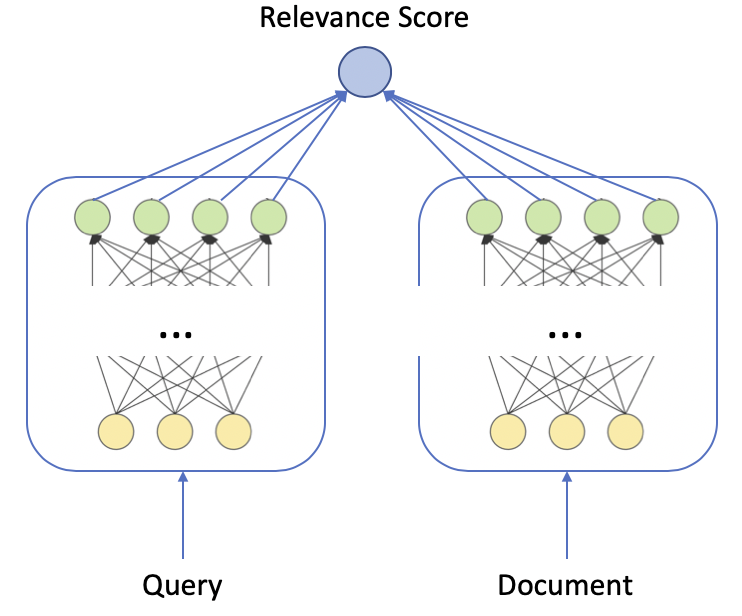
\includegraphics[width=\linewidth]{Figures/representation-based.png}
% %   \captionof{figure}{A figure}
% %   \label{fig:representation_based}
% \end{minipage}
% \begin{minipage}{.45\textwidth}
%   \centering
%   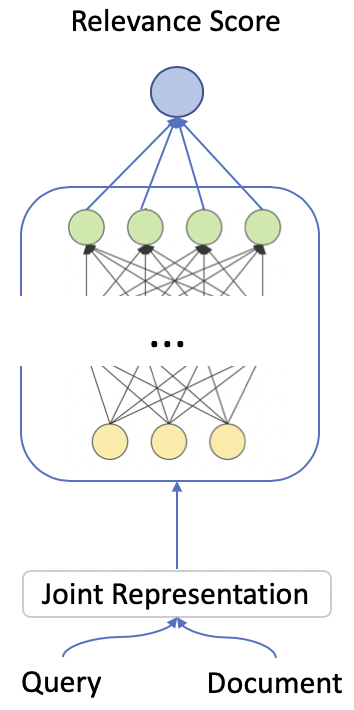
\includegraphics[width=0.5\linewidth]{Figures/interaction-based.png}
% %   \captionof{figure}{Another figure}
% %   \label{fig:interaction-based}
% \end{minipage}
% \caption{Example of \textit{representation-based} model (left) and \textit{interaction-based} model (right).}
% \label{}
% \end{figure}

\begin{figure}
    \centering
    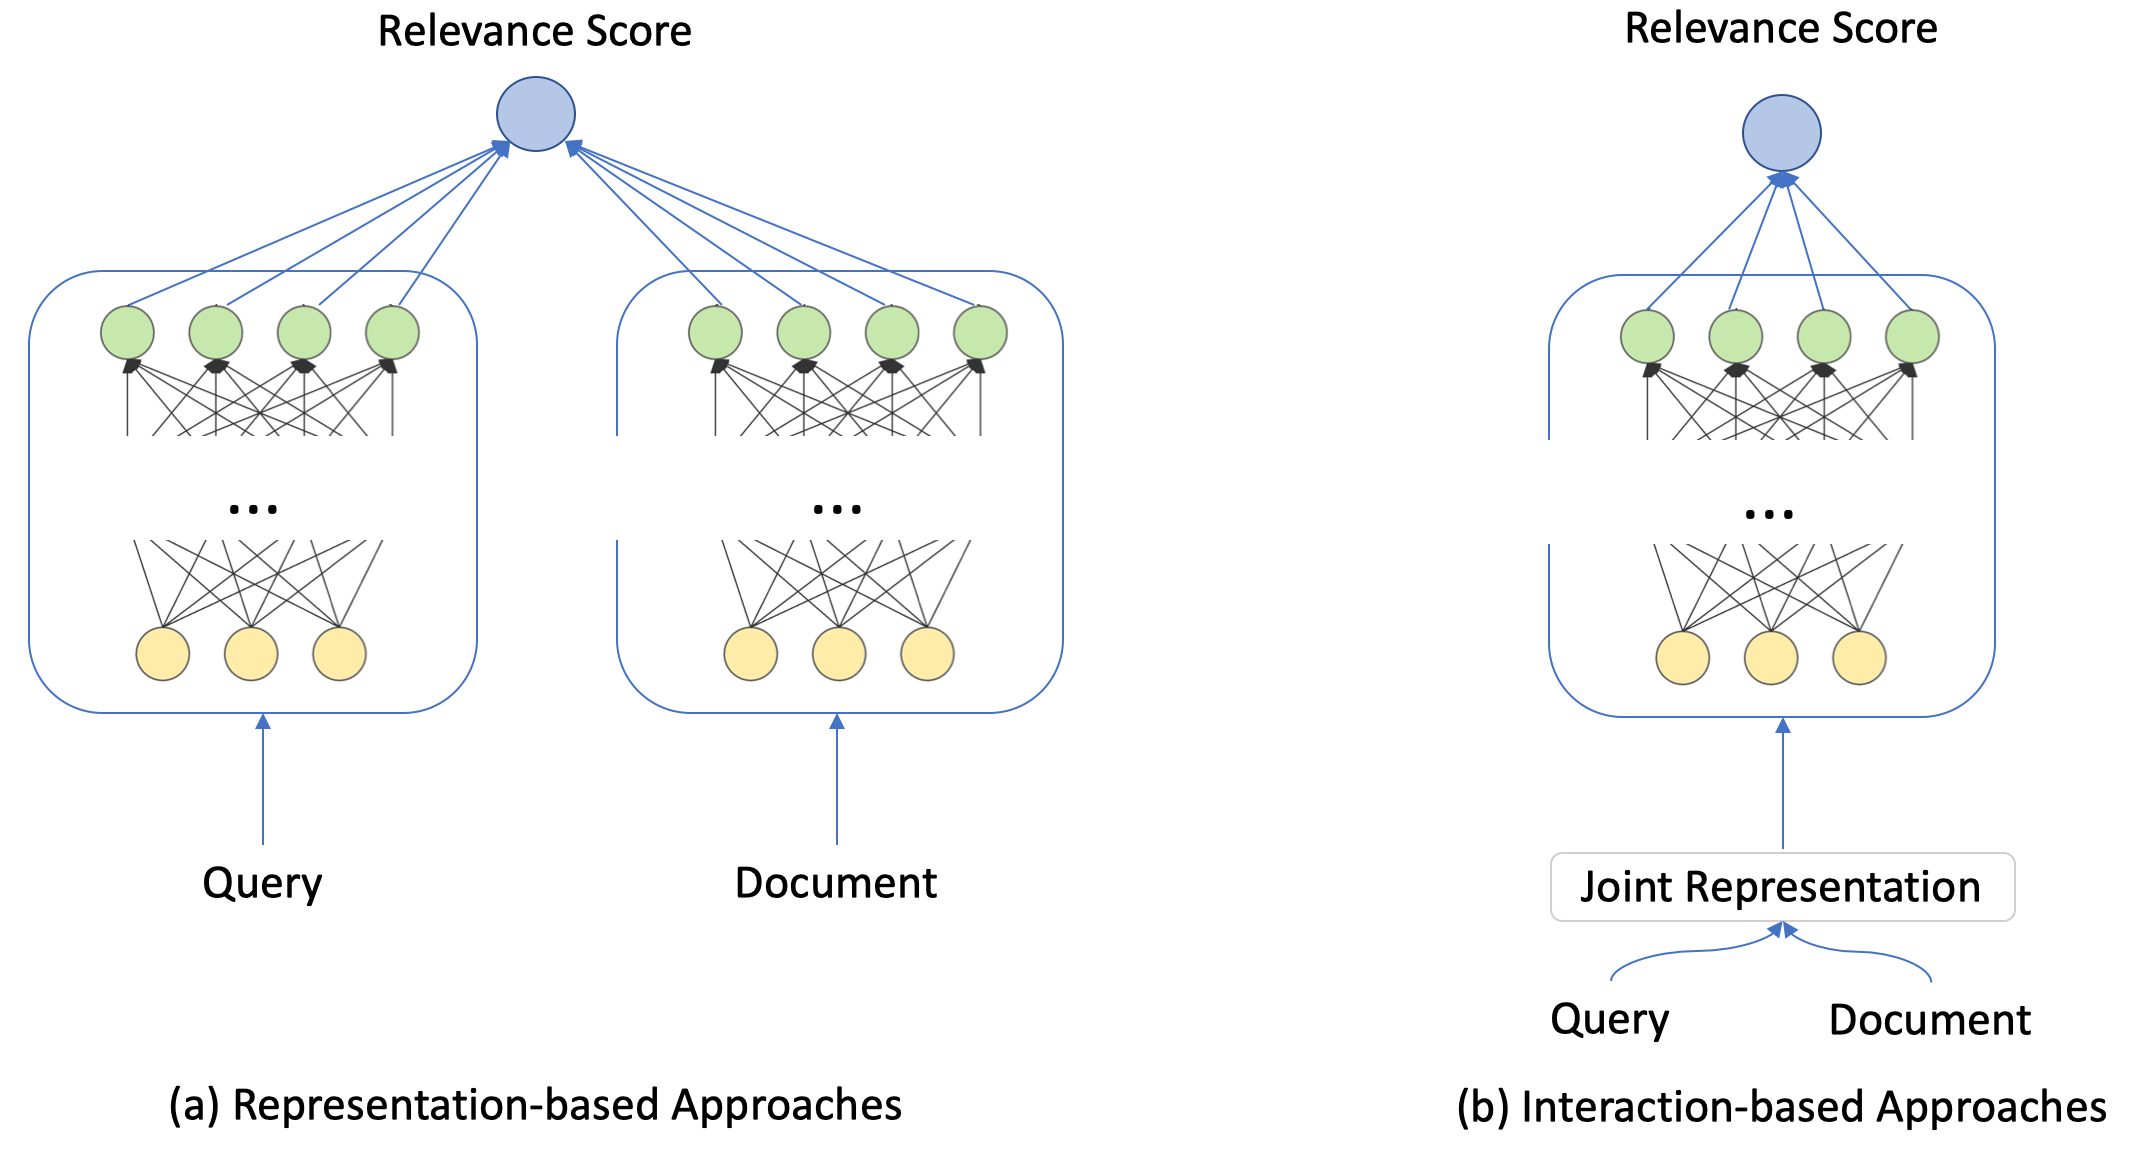
\includegraphics[width=0.7\textwidth]{Figures/neural_ir_types.png}
    \caption{Types of Neural Network Architectures for IR.}
    \label{fig:neural_ir_types}
\end{figure}

In \textit{representation-based} models (section~\ref{sec:representation_based}), the focus is on learning meaningful semantic representations of the text through several hidden layers using a deep neural network (DNN) and estimating the relevance score by using a matching function on the last level representations of the query and document. In this approach, $\Phi$ is a complex representation mapping function and $F$ is a simple matching function like cosine or dot similarity. For example, in DSSM~\citep{dssm13}, $\Phi$ is a feed forward neural network and $F$ is cosine similarity.

In \textit{interaction-based} models (section~\ref{sec:interaction_based}), the focus is on learning salient interaction patterns from the local interactions between the query and document that is fed as input into a DNN. In this approach, $\Phi$ is a simple mapping function while $F$ is a complex deep model. For example, in DRMM~\citep{Guo2016}, $\Phi$ is maps each text into a sequence of word vectors and $F$ is a feed forward neural network over the interaction matrix built from the word vectors of the two texts.

Whereas, in DUET~\citep{Mitra2017a} they combine both \textit{representation-based} and \textit{interaction-based} models by employing two separate deep neural network models--\textit{local} model that estimates the relevance score according to exact matches between query and document terms, and \textit{distributed} model that estimates relevance by matching dense lower-dimensional representations of both query and document text. The final relevance score is the sum of scores obtained from the two sub-networks. They carry out experiments on commercial search log data from Bing and compare their approach against traditional baselines (BM25, QL, DM) and neural baselines (DRMM, DSSM, CDSSM, DESM) and show that it largely outperforms the baselines. 

\subsection{Representation-Based Models}
\label{sec:representation_based}
The \textsf{Deep Structured Semantic Model} (DSSM)~\citep{dssm13} is the earliest work in neural \textit{representation-based} models for ad-hoc retrieval. The DSSM model is composed of a deep neural network with three non-linear layers on top of a word hashing layer. The query and document are first mapped to high-dimensional term vectors (\textit{bag-of-words} representation). After this the term vectors are mapped to trigram vectors by the word hashing layer, in order to cope with the large size of the vocabulary (reduces vocabulary size from 500K to 30K).

In \textsf{Convolutional Deep Structured Semantic Model} (C-DSSM)~\citep{Shen2014b} they extend DSSM by including a convolutional neural network (CNN) with max-pooling followed by a semantic layer to get high level representations of text. It first uses word hashing to project each word into a tri-gram vector. Then the convolutional layer projects each word vector within a context into a local contextual vector. Following which max-pooling is applied that picks the most salient local features to form a fixed-length global vector for queries and documents. Since both DSSM and C-DSSM fail to capture contextual information accurately,~\cite{Shen2014a} propose a \textsf{Convolutional Latent Semantic Model} (CLSM) that is built on top of DSSM. In this, the first layer consists of \textit{word-n-grams} constructed using a contextual sliding window over the input word sequence followed by letter tri-gram representation that maps each word-n-gram to its tri-gram representation like in DSSM. Then, a convolutional layer transforms these tri-grams into contextual feature vectors using a convolutional matrix shared between the word-n-grams. Then, max-pooling is applied against each dimension of the contextual feature to pick salient word-n-grams to form a fixed length vector. Finally, a semantic layer performs a non-linear transformation to obtain a semantic representation of the text. 

All of the above models are trained and evaluated on large-scale datasets from Bing. The models are discriminatively trained on query-document title pairs from the clickthrough data such that the conditional likelihood of the clicked document for a given query is maximized (\textit{cross-entropy} loss). These models are shown to outperform baselines comprising of Word Translation Model, TF-IDF, BM25 in terms of retrieval effectiveness (NDCG @1,3,10). However, in a later work~\citep{Guo2016} they show that both DSSM and C-DSSM do not perform as well as traditional IR models when using the entire document body.

In recent work~\citep{Nie_ictir18}, they compare a representation-based approach (C-DSSM without word transformation to tri-letter representation) and interaction-based approach (MatchPyramid but with additional CNN layer) under the same test conditions (experimental setup) using weak supervision~\citep{Dehghani_sigir17} (section \ref{sec:weak_supervision_ir}) with AOL query logs to generate a large amount of training data to be able to reasonably train both models on the ClueWeb09-Cat-B collection. However, their experimental results are inconsistent with that of~\cite{Dehghani_sigir17}, where they show that a neural model based on representation learning, weakly supervised by BM25, can give better retrieval effectiveness than the BM25 baseline. This could be due to the difference in dense input representation, where in~\cite{Dehghani_sigir17} they concatenate the IDF weighted element-wise sum of the term's embedding vectors of both the query and document. Finally, in~\cite{Nie_ictir18} to improve the retrieval effectiveness of the representation-based model, they employ matching at different levels of abstraction instead of a matching applied on the representation obtained from the final layer for computing a relevance score like in previous works. They build interaction matrices from the embeddings or convolved vectors between the query and document at each layer and then pick the strongest $p$ signals across each row, average it and then sum up the averages of every query representation to get a matching score for that layer. These matching scores are aggregated through a softmax gate to get a global matching score for the query and document.

In~\cite{Ai2016a,Ai2016b} they investigate the use of \textsf{PV-DBOW}~\citep{Le2014} as a document language model for retrieval. They propose three improvements over the original model for retrieval: (1) use document-frequency based rather than corpus-frequency based negative sampling so that frequent words will not be suppressed too much; (2) regularization over document representation to prevent model overfitting to short documents; and (3) joint-learning objective that considers both document-word and word-context associations to better model word substitution relations. They show higher effectiveness over LDA-based LM and QL for Robust04 and GOV2 collections.

\subsection{Interaction-Based Models}
\label{sec:interaction_based}

\subsubsection{Bag-of-words based} 
\textsf{Deep Relevance Matching Model} (DRMM)~\citep{Guo2016} is one of the first \textit{interaction-based} models to show improvements over traditional IR models (bag-of-words baselines). The query-document local interactions are first mapped into fixed-length \textit{matching histograms} to distinguish between exact matching and soft matching signals using term embedding cosine similarities. These signals are fed into a \textit{feed forward} NN and a \textit{term-gating} network that models term importance to finally get a relevance score for the query-document pair. In their experiments over Robust04 and ClueWeb-Cat-09B collections, they show significant improvements over the baselines: BM25, QL, representation-based models (DSSM, C-DSSM) and interaction-based models (MatchPyramid). The term embeddings are trained on the respective collections and they also show empirically that as the CBOW dimensions increases, the DRMM performance first increases and then slightly drops.

Similar to DRMM, \textsf{Kernel-based Neural Ranking Model} (K-NRM)~\citep{KNRM17} first creates a query-document interaction matrix that computes the cosine similarity between the term embeddings of both query and document. Then, they use multiple \textit{gaussian kernels} to obtain different levels of exact and soft-matching features from the interaction matrix which is then used as an input to a ranking layer which is a linear layer with \textit{tanh} activations to produce the final relevance score. The model is trained end-to-end using a max-margin learning-to-rank loss function. During \textit{learning}, the kernels convert the loss and adjust the word embeddings to produce a soft matching signal that better seperates relevant and irrelevant documents. They conduct extensive experiments on a Chinese commercial search engine query logs (Sogou) and show significant improvement over traditional baselines (BM25), learning-to-rank approaches (RankSVM) and neural IR baselines (DRMM, C-DSSM). They also carry out an analysis that shows using a model without multi-level soft matches or embedding learning (using pre-trained \texttt{word2vec} embeddings) quickly diminishes the performance of K-NRM.

\subsubsection{Word n-gram based}
\textsf{MatchPyramid}~\citep{matchpyramid16} is one of the first works that tries to capture hierarchical matching patterns based on \textit{n-gram} matches from the local interaction matrix of the query-document. They employ a convolutional neural network (CNN) comprising of one convolutional layer and dynamic max pooling layer on top of the interaction matrix to extract hierarchical matching patterns. Finally, the output of the CNN is fed into a MLP to produce a ranking score. They conducted extensive experiments to study the impact of pooling sizes, similarity functions (cosine, indicator, gaussian) and kernel sizes on the retrieval performance on the Robust04 collection. They achieve a better retrieval performance over traditional IR models (BM25, QL), and representation-based models (pretrained DSSM, C-DSSM), using a pooling length equivalent to paragraphs, a similarity function that differentiates between exact and semantic matches and small kernel size. 

In \textsf{Multi-level Abstraction Convolutional Model} (MACM)~\citep{Nie_ictir18, Nie_sigir_2018}, they use a model similar to MatchPyramid but with an additional convolutional and max-pooling layers and integrates the matching scores at different levels of abstraction. They determine matching scores at each abstraction level by flattening the max-pooled layer and using a MLP to obtain a score. The matching scores are aggregated through a softmax gating mechanism that considers the importance of each abstraction level by computing the max interaction values across each row of the interaction matrix or convolution feature maps and then summing up these max interaction values to get a global importance value. They show that the model trained with weak supervision using AOL query logs can outperform BM25 baseline on the ClueWeb-Cat-09B collection. They also compare with model variants without multi-level matching like in MatchPyramid and show that it outperforms these variants as well.

\textsf{Convolutional Kernel-based Neural Ranking Model} (Conv-KNRM)~\citep{ConvKNRM18} improves upon the K-NRM model by employing CNN to compose adjacent word embeddings into n-gram embeddings. The n-gram embeddings from both query and document can be combined into multiple interaction matrices that allows cross-matching of n-grams of different lengths. They then use the kernel pooling and ranking layer to combine the n-gram soft matches into a final ranking score~\citep{KNRM17}. They conducted experiments using English search logs from Bing (WSDM'09 workshop) and Chinese search logs from Sogou and show the advantages of this approach over the baselines: BM25, RankSVM, DRMM, C-DSSM, MatchPyramid and K-NRM. They also carry out experiments on ClueWeb-Cat-09B collection, where they use a domain adaptation method as there isn't sufficient training data. So, they pre-trained Conv-KNRM using the Bing search logs to be able to train the word embedding and convolutional layers effectively and then they use the relevance judgements from TREC 09-12 web tracks to re-train the soft matching kernel pooling and ranking layer keeping the embedding and convolutional layers `frozen'. This approach is shown to outperform all of the baselines mentioned above.

In \textsf{Position-Aware Convolutional Recurrent Relevance model} (PACRR)~\citep{pacrr17}, they use a combination of convolutional kernels to capture interactions that includes unigrams, bi-grams and tri-grams matches; $k$-max pooling along the query dimension to preserve important signals from different query terms; and recurrent layer to combine signals from different query terms to produce a global relevance assessment. Later, they improve on PACRR and introduce Co-PACRR~\citep{co_pacrr_wsdm18} which is a context-aware variant that takes into account the local and global context of the matching signals. For this they use three components:(1) \textit{disambiguation} component for considering the matching signal with the local context in which it occurs, this is done by introducing an input that captures the similarity between the query vector and all document contexts defined by a window; (2) \textit{cascade k-max pooling} to account for the location of matching signals by applying $k$-max pooling at multiple positions in the document instead of pooling on the entire document; (3) \textit{shuffling combination} layer to regularize the model so that it doesn't learn the absolute position of terms within the query as this could influence the aggregation layer to down-weight positions that are generally zero padded. They compare their approaches with state-of-the-art neural models including DRMM, K-NRM, local model of DUET and MatchPyramid on six years of TREC WebTrack benchmarks and show significant improvements over all baselines. They also note that their approach after re-ranking QL ranked results produce runs that are ranked within the top-3 runs on atleast 5 years based on ERR@20. %They perform an abalation analysis on the proposed components in Co-PACRR to gain insights about its usefulness. 

In~\cite{pacrr_drmm_18}, they propose several extensions to DRMM so as to account for the context in which the query terms appear. First, they introduce PACRR-DRMM a simple model that uses DRMM to independently score each of the (document-aware) query term encodings that are obtained from PACRR and aggregates these scores using a linear layer. They then propose two additional models that uses \textit{context-sensitive} term embeddings obtained from pre-trained embeddings by using a standard BiLSTM encoding scheme: (1) \textsf{Attention-Based ELement-wise} DRMM (ABEL-DRMM) in which a document representation for each q-term ($d_{q_i}$) is first computed by taking a sum of the context-sensitive encodings of d-terms, weighted by their attention score that is computed using a softmax over the dot product between that q-term and d-term encoding and then the (document-aware) q-term encoding is the hadamard product between $d_{q_i}$ and q-term encoding; (2) \textsf{POoled SImilariTy DRMM} (POSIT-DRMM) in which document-aware q-term encoding is computed by first concatenating attention scores that are obtained from cosine similarity between q-term and d-term encodings and then creating a representation that includes the max-pooled attention score and average of the $k$-max pooled attention scores. They compare against BM25, and neural IR baselines (DRMM, PACRR) on the TREC Robust04 collection and show significant improvements over all baselines.

\subsubsection{Document context based}
\textsf{DeepRank}~\citep{Pang_deeprank_2017} proposes a new architecture that better models the human judgement process while assigning relevance to a query-document pair. The model first employs a \textit{detection strategy} to extract query-centric contexts from the document, that is, the contexts with a query term in the center. Then the \textit{measure network} determines the local relevance between query and query-centric contexts by creating an 3D input tensor that includes query, and query-centric word representations along with the word-level interaction matrix between the word embeddings of the query \& query-centric context (cosine/indicator). They then use either a CNN or 2D gated recurrent unit (2D-GRU) to capture the local relevance from the input tensor producing a \textit{local relevance vector} containing matching patterns extracted from different kernels. Finally, the \textit{aggregation network} aggregates the local relevances at a query term level, and then combines it by weighting the query term importance using a term gating mechanism. The query-term level relevance is computed by first grouping the query-centric contexts that have the same query word together and then using a RNN to aggregate these local relevance vectors sequentially which also considers the position of the query-centric contexts in the document. They conduct experiments on both benchmark LETOR4.0 data (MQ2007, MQ2008) and large scale Chinese clickthrough data (Sogou). The experimental results show that: (1) Existing neural IR models such as DSSM, CDSSM, DRMM perform worse than the pairwise (RankSVM, RankBoost) and listwise (ListNet, AdaRank, LambdaMart) learning-to-rank methods using hand-crafted features; (2) DeepRank significantly improves the performance across both existing NRMs and learning-to-rank baselines.

Building upon DeepRank,~\cite{Fan_hint_2018} propose a \textsf{HIerarchical Neural maTching model} (HiNT) to learn diverse relevance patterns by a data-driven approach to allow relevance signals from different granularities (document-wide or passage-level) compete with each other to obtain a final relevance score. The model consists of two stacked components: (1) \textit{local matching layer} which produces a set of local relevance scores between a query and each passage of a document (obtained by a fixed-sized sliding window). The relevance scores are computed by building two 3D input tensors as described in ~\cite{Pang_deeprank_2017}--one for exact matching and one for semantic matching and both are given as input to a 2D Gated-RNN (spatial GRU) and the last hidden representation is taken as the matching output; (2) \textit{global matching layer} is a hybrid network that aggregates passage level relevance at different granularities--\textit{independent decision} model assumes that the passage-level relevance scores are independent and \textit{accumulative decision} model applies LSTM sequentially across the passage-level signals to generate an accumulated relevance scores at different positions. Then, $k$-max pooling is applied over the dimensions to pick the top-$k$ signals from either the passage-level or accumulated relevance signals, which is then concatenated as input to a MLP for the final relevance score. They follow a similar experimental setup as~\cite{Pang_deeprank_2017} and show improvements over traditional document-wide, passage-level retrieval models, learning-to-rank methods and neural IR models. 

In \textsf{DeepTileBars}~\citep{deeptilebars_2019}, they first split the documents into topical segments using the TextTiling algorithm~\citep{Hearst_text_tiling_94} which splits documents at positions where a change in topic is detected and they then create a query-segment interaction matrix which is fed into the neural IR  model (DeepTileBars) to obtain a relevance score. Each cell in the query-segment interaction matrix comprises of 3 values--term frequency of query word in segment, inverse document frequency of query word, and similarity score (gaussian kernel) of most similar word in the segment using word embeddings. DeepTileBars first has multiple CNNs with different kernel sizes that are employed to learn relevance patterns at different levels of granularity in the document's topic hierarchy. Then LSTMs of the same number as CNNs are used accumulate the relevance signals from the output of the CNNs, this gives relevance scores of the document at different granularities. All the different relevance scores are aggregated using a MLP to get a final global relevance score for the document. They conduct experiments on the TREC WebTrack (2010-12) and LETOR4.0 (MQ2008) and show improvements over traditional IR baselines (BM25, QL) and neural IR baselines (DRMM, MatchPyramid, DeepRank, HiNT).

\subsection{Weak Supervision for Neural IR}
\label{sec:weak_supervision_ir}
Recently, \cite{Dehghani_sigir17} propose a \textsf{weak supervision} method to use large amounts of unsupervised data to generate `weak' labels that can be used as a signal to learn neural IR models. They examined neural ranking models with different architectures, training objectives (pointwise, pairwise), and different input representations from encoding query-document pairs into sparse or dense vectors to learn dense embeddings for each text. The models are trained on billions of training examples obtained by using AOL query logs as a query set and retrieving \textit{pseudo-relevant} documents for each query using BM25 (weak supervision signal). They observed that by using just the training data obtained from the BM25 weak annotator they are able to outperform BM25 on the test dataset. This is the case only with the models that uses an embedded vector representation which concatenates the weighted element-wise sum of the term embeddings from the query and document. They also carry out analysis to understand what the model learns, if the use of pretrained embeddings from external/target corpus instead of learnt embeddings affects the performances of the models. They demonstrate that training a model with limited amount of supervised data (relevance judgements) after pre-training it on weakly supervised data gives a significant improvement in performance. This approach has been used lately to train various neural ranking models~\citep{Nie_ictir18, Nie_sigir_2018, Bo_coling18, Zamani_neural_reranking_2018}. Most recently,~\cite{Zamani_weak_sup_theory_2018} provided a theoretical foundation for explaining the successful empirical results achieved by weakly supervised neural IR models. 

``\textsf{Fidelity-Weighted Learning}''~\citep{dehghani_nips17, dehghani2018fidelityweighted} is a semi-supervised student-teacher approach for training deep neural networks with weakly supervised data instead of treating the weakly labeled samples uniformly. The \textit{student} network is initially trained on weak data to learn an initial task-dependent data representation (embedding dense vector representation in \cite{Dehghani_sigir17}). This data representation is then used with the \textit{teacher} network which is a Bayesian semi-supervised approach that learns to predict the strong data (limited relevance judgements). Then, the \textit{teacher} is used to generate a new weakly supervised data with confidence scores for each pair of data. This new weak dataset is used to fine tune the parameters of the student network. The experiments on Robust04 and ClueWeb-Cat-09B show that this approach provides improvements over the weakly supervised setup in~\cite{Dehghani_sigir17}. %The experiments on Robust04 and ClueWeb-Cat-09B, show that this approach provides significant improvements over BM25 and the weakly supervised setup in~\cite{Dehghani_sigir17}.

\subsection{Neuro-Pseudo Relevance Framework for Neural IR}
\label{sec:npr_ir}
Recently, in ~\cite{li2018nprf} they propose a \textsf{Neuro Pseudo Relevance Framework} (NPRF) that enables the use of pseudo relevance feedback with existing neural IR models. The existing neural IR models are used as scorers to evaluate the target document with respect to the top-ranked queries and the query without changing their architectures. They show two examples of the NPRF framework with two neural IR models--DRMM and KNRM, and evaluate their performance on TREC benchmark datasets (TREC 1-3, Robust04) for ad-hoc retrieval. A brief description of the architecture is given in section~\ref{sec:nprf_drmm_reproducibility_desc} and we detail the reproducibility experiments on TREC Robust04 collection that we carried out on the NPRF-DRMM variant from this paper in section~\ref{sec:nprf_drmm_reproducibility_exp}.

\subsection{Learning Sparse Representations for Indexing}

In~\citep{Zamani_neural_reranking_2018} they propose a \textsf{Standalone Neural Ranking Model} (SNRM) that can retrieve relevant documents from a large-scale collection, instead of re-ranking a small set of candidate documents that are retrieved by a first stage ranker (BM25, QL) which is the approach used in all previous neural ranking models. They propose a network architecture to learn \textit{latent sparse} representations for each continuous $n$ words of both queries and documents in the same semantic space. The learned sparse representations of n-grams are then aggregated using average pooling to get a sparse representation for the entire text. The fully connected feed forward network has a hourglass structure with small number of units in the middle layers to learn a low-dimensional representation of the data and the upper layers have a large number of units to get a sparse output representation from the sequence of $n$ embedding vectors concatenated (n-gram). These sparse representations are trained with weak supervision using a training objective that is a combination of pairwise max-margin loss and sparsity objective that minimizes the $L_1$-norm of the sparse representations. After training, the inverted index is constructed by considering each index of the learned representation ($\phi$) as a ``latent'' term, so then for each document in the collection if the $i^{th}$ index of $\phi_D$(d) is non-zero, it is added to the inverted index for the latent term $i$. During inference, the query sparse representation $\vec{q}$ is first obtained and for each non-zero element in $\vec{q}$ the corresponding documents from the inverted index are retrieved and scored using the dot product. 
% \section{Dual Embedding Space Model (DESM)}
% When using word embeddings for IR it is more appropriate to represent query terms using IN embeddings and documents terms using OUT embeddings of the trained model as it captures $aboutness$ aspect of document ranking. In this model\citep{Nalisnick:2016,Mitra2016a}, word2vec is trained on search queries instead of document body text as it empirically performs better. Training on short queries makes inter term similarity more pronounced when using both terms represented as IN vectors. While using IN-OUT vectors for terms gives a better topical notion of relatedness which is better for retrieval.

% The \textit{Continuous Bag-of-Words} (CBOW) model~\citep{Mikolov2013} with negative sampling is used to learn the word embeddings as its able to capture word co-occurrences. The model predicts word $w_i$ by adapting its representation vector such that it has a large inner product with the mean of the context word vectors.

% The ranking function based on the learnt embeddings is defined as
% \begin{align}
%     DESM(Q,D) = \
%     \frac{1}{|Q|}\sum_{q_i \in Q}{}\frac{ q_i^T{\bar{D}}}{\|q_i\|\|{\bar{D}}\|} \\
%     \intertext{where}
%     \bar{D} = 
%     \frac{1}{|D|}\sum_{d_j \in D}{}\frac{d_j}{\|d_j\|}
% \end{align}

% Here $\bar{D}$ is the centroid of all the normalized vectors for the words in the document which represents a single embedding for the whole document.

% \textbf{Training corpus}. The CBOW model is trained on a query corpus consisting of 6 million queries and having a vocabulary size of 2.7 million words. All experiments are repeated using another CBOW model trained on document body text with 341 million distinct sentences sampled from Bing search index having a vocabulary of 5.1 million words.

%-----------------------------------------------------
%	SECTION 3
%-----------------------------------------------------
% \section{DUET Architecture}
% A document ranking model composed of two separate deep neural networks, one that matches query and document using local representations (local model) and one that matches them using distributed representations (distributed model)~\citep{Mitra2017a}. Both these deep neural networks are jointly trained as part of a single neural network. The final score under the architecture is the sum of scores from individual networks,
% \begin{equation}
%     f(Q,D) = f_l(Q,D) + f_d(Q,D)
% \end{equation}
% where query and document are ordered list of terms, Q = [$q_1,...,q_{n_q}$] and D = [$d_1,...d_{n_d}$]. Each term is represented as a one-hot vector of $m_l$ dimension, where $m_l$ is the size of the vocabulary. The length of the inputs across all queries and documents are fixed, such that, only the first 10 terms in the query and first 1000 terms in the document are considered.
% \begin{figure*}
%     \centering
%     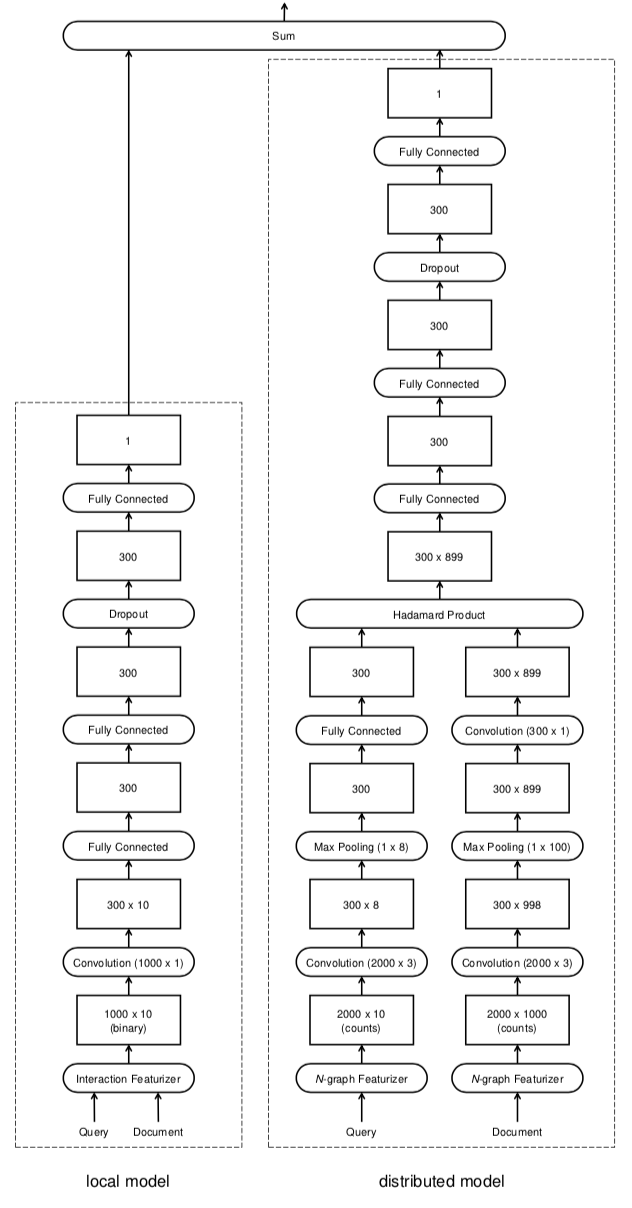
\includegraphics{Figures/DUET.png}
%     \caption{DUET architecture. The local model takes query-document interaction matrix as input, whereas distributed model learns embeddings of query and document text before matching. The parameters of both models are jointly optimised.}
%     \label{fig:duet_architecture}
% \end{figure*}

% \textbf{Local Model}. The model estimates document relevance based on exact matching patterns between query terms in the document. The interaction matrix is a $n_d * n_q$ binary matrix $X = D^TQ$, that captures every exact match of query terms in the document. The matrix is passed through a convolutional layer with $c$ filters, a kernel size $n_d * 1$ and stride of 1. The output $Z$ of the convolutional layer (eq.~\ref{eq:conv_layer_eq_duet}) is then passed through two fully connected layers, a dropout layer and a final fully-connected layer that gives a single score. All nodes in the local model uses hyperbolic tangent for non-linearity.
% \begin{align}\label{eq:conv_layer_eq_duet}
%     \mathrm{Z_i} = \tanh(\mathrm{X}_i^T\mathrm{W})
% \end{align}
% where W is $n_d * c$ matrix of learnable parameters.

% \textbf{Distributed Model}. This model learns a dense lower-dimension vector representations of both query and document, before computing the positional similarity between them in the embedding space. Character $n$-graph based representation of each term in the query and document is used. For each term, all the $n$-graphs present for $1 \leq n \leq G$ is counted, where G is set to 5. This $n$-graph frequency vector of length $m_d$ is used to represent the term ($m_d = 2000$, which is the top-2000 most popular $n$-graphs).

% In this model, the $Q$ matrix $m_d*n_q$ and $D$ matrix $m_d*n_d$ are sent to a convolutional layer of window ($m_d*3$) and filter size of 300. This layer generates a tensor of dimension $300*8$ for the query, and $300*998$ for the document. Following this there is max-pooling layer. For the query, the pooling kernel dimension is $1*8$, to get one query matrix $\widetilde Q$ ($300*1$). For the document, the pooling kernel is $1*100$ to generate a matrix $\widetilde D$ ($300*899$). The window based max pooling strategy helps distinguish between matches in different parts of the document. The combination of convolutional, max-pooling and fully-connected layers enables the model to learn suitable representations of text for effective inexact matching. Finally the matching is performed using an element-wise product between embedded document matrix and broadcasted query embedding.
% \begin{align*}
%     \widetilde X = (\underbrace{\widetilde Q...\widetilde Q}_\text{899 times})\circ\widetilde D
% \end{align*}

% \textbf{Training Objective}. Each training sample consists of a query, relevant document and set of non-relevant documents. Softmax function is used to compute posterior probability of relevant document given a query based on the score.
% \begin{align*}
%     p(D^*|Q) = \frac{\exp (f(Q,D^*))}{\sum_{D \in N} \exp (f(Q,D))}
% \end{align*}

% \begin{sidewaystable}
%     % \centering
%     \footnotesize
%     \scalebox{0.65}{
%     \begin{tabular}{m{5em}m{7em}m{7em}m{7em}m{7em}m{7em}m{7em}m{7em}m{7em}m{7em}m{7em}m{7em}m{7em}}
%     \toprule
%          & DESM & DUET & DSSM & CDSSM & DRMM & MatchPyramid & PACRR \newline Co-PACRR & K-NRM & MACM & Conv KNRM & DeepRank & FNRM \newline \cite{Dehghani_sigir17}\\
%          \midrule
%         I/P Repr. & BOW\newline+\newline Embeddings & query-doc interaction matrix \newline query and doc tri-gram vector & Bag-of-character tri-gram vector & Bag-of-character tri-gram vector & query-doc interaction matrix (cosine) &
%         query-doc interaction matrix (cosine, ind.,\newline dot, gaussian) &
%         query-doc interaction matrix (cosine) & query-doc interaction matrix (cosine) & query-doc interaction matrix (cosine)\\
%         \addlinespace[1em]
        
%         Training workload & --- & click-through data \newline 200K Bing & click-through data \newline 16K Bing & click-through data \newline 16K Bing & judgements \newline Robust04 Track \newline CW WebTrack 09-11 & judgements \newline Robust04 Track & judgements \newline CW \newline WebTrack 09-14 & click-through data 100K Sogou (Chinese) & AOL query logs (weak sup.)\\
%         \addlinespace[1em]
        
%         Word Embeddings & \texttt{CBOW} \& \texttt{SGNS} Bing & --- & --- & --- & \texttt{CBOW} \newline Robust04 & \texttt{Glove} Wikipedia & \texttt{word2vec} GoogleNews & --- & \texttt{Glove} Wikipedia\\
%         \addlinespace[1em]
        
%         Evaluation Testset & Bing Prop. \newline Robust04, CW & Bing Prop. & Bing Prop. & Bing Prop. & Robust04, CW & Robust04 titles & CW WebTrack 09-14 & Sogou Prop. & CW WebTrack 09-12\\
%         \addlinespace[1em]
        
%         Impl. Trainable & \checkmark & weak sup. & weak sup. & weak sup. & \checkmark & \checkmark & \checkmark & \checkmark & weak sup.\\
%         \addlinespace[1em]
        
%         OOV \newline handling & skips & \xmark & \xmark & \xmark & Ind. match 1/0 & NA. & Retrain unseen words & \xmark & skips\\
%         \addlinespace[1em]
        
%         Baselines & BM25, LSA & BM25, LSA, \newline QL, DRMM, \newline DSSM, CDSSM, DESM & BM25, LSA, \newline DAE & BM25, LSA,\newline DSSM & QL, BM25, \newline DSSM, CDSSM, MP & QL, BM25, \newline DSSM, CDSSM & DUET-L, KNRM, DRMM, MP & BM25, QL, \newline DSSM, CDSSM, \newline DRMM, RankSVM & BM25, QL\\
%         %\addlinespace[1cm]
        
%         Training Obj. & --- & log-likelihood & cross entropy & cross entropy & max margin & max margin & max margin \newline Co-PACRR (cross entropy) & max margin & max margin\\
%     \bottomrule
%     \end{tabular}}
%     \caption{Comparison of Neural IR model architectures and experimental setups.}
%     \label{tab:neuir_comparison}
% \end{sidewaystable}

% \pagebreak
{
    \centering
    \tiny
    % \scalebox{0.63}{
    %{lm{7em}m{7em}m{7em}m{7em}m{7em}m{5em}m{7em}m{5em}}
    \begin{longtable}{C{3.7em}m{7em}C{5em}C{4em}m{4.5em}C{4.2em}C{3.5em}m{7.1em}L{3.5em}}
    \addlinespace[1em]
    \toprule
    \addlinespace[2em]
    \caption[]{Comparison of Neural IR model architectures and experimental setups. (continued)}
    \endfoot
    \caption{Comparison of Neural IR model architectures and experimental setups.}
    \endlastfoot
    \toprule
    Model & I/P Repr. & Training workload & Word \newline Embeddings & Evaluation Testset & Impl. Trainable & OOV \newline handling & Baselines & Training Obj.\\
    \midrule
    \endhead
        
        DESM & BOW +\newline Embeddings & --- & \texttt{CBOW} \& \texttt{SGNS} Bing & Bing Prop., \newline Robust04, CW & \checkmark & skips & BM25, LSA & ---\\
        \addlinespace[0.5em]
        \midrule
        \addlinespace[0.5em]
        
        DUET & query-doc interaction matrix \newline query \& doc \newline tri-gram vector & click-through data \newline 200K Bing & --- & Bing Prop. & weak sup. & \xmark & BM25, LSA, \newline QL, DRMM, \newline DSSM, CDSSM, DESM & log-likelihood\\
        \addlinespace[0.5em]
        \midrule
        \addlinespace[0.5em]
        
        DSSM & Bag-of-character tri-gram vector & click-through data \newline 16K Bing & --- & Bing Prop. & weak sup. & \xmark & BM25, LSA, \newline DAE & cross \newline entropy\\
        \addlinespace[0.5em]
        \midrule
        \addlinespace[0.5em]
        
        CDSSM & Bag-of-character tri-gram vector & click-through data \newline 16K Bing & --- & Bing Prop. & weak sup. & \xmark & BM25, LSA, \newline DSSM & cross \newline entropy\\
        \addlinespace[0.5em]
        \midrule
        \addlinespace[0.5em]
        
        DRMM & query-doc interaction matrix (cosine) & judgements \newline Robust04, CW WebTrack 09-11 & \texttt{CBOW} \newline Robust04 & Robust04, CW & \checkmark & Ind. match 1/0 & QL, BM25, \newline DSSM, CDSSM, MP & max \newline margin\\
        \addlinespace[0.5em]
        \midrule
        \addlinespace[0.5em]
        
        MatchPyr. MP & query-doc interaction matrix (cosine, ind., dot, gaussian) & judgements Robust04 & \texttt{Glove} Wikipedia & Robust04 titles & \checkmark & NA.\footnote{Not mentioned in the paper.} & QL, BM25, \newline DSSM, CDSSM & max \newline margin\\
        \addlinespace[0.5em]
        \midrule
        \addlinespace[0.5em]
        
        PACRR \newline Co-PACRR & query-doc interaction matrix (cosine) & judgements CW WebTrack 09-14 & \texttt{word2vec} GoogleNews & CW WebTrack 09-14 & \checkmark & Retrain OOV words & DUET-L, KNRM, DRMM, MP & max \newline margin \newline Co-PACRR (cross entropy)\\
        \addlinespace[0.5em]
        % \midrule
        % \addlinespace[0.5em]
        
        K-NRM & query-doc interaction matrix (cosine) & click-through data 100K Sogou (Chinese) & Trained with model & Sogou Prop. & weak sup. & \xmark & BM25, QL, \newline DSSM, CDSSM, DRMM, RankSVM & max \newline margin\\ 
        \addlinespace[0.5em]
        \midrule
        \addlinespace[0.5em]
        
        Conv-KNRM & query term embed matrix \& doc term embed matrix & click-through data \newline 100K Sogou, \newline 100K Bing, \newline CW 09-12 & Trained with model & Sogou Prop., \newline Bing Prop.,\newline CW 09-12 & weak sup. & \xmark & BM25, MP,\newline DRMM, CDSSM, KNRM, RankSVM & max \newline margin\\
        \addlinespace[0.5em]
        \midrule
        \addlinespace[0.5em]
        
        MACM & query-doc interaction matrix (cosine) & AOL query logs \newline (weak sup.) & \texttt{Glove} Wikipedia & CW 09-12 & weak sup. & skips & BM25, QL & max \newline margin\\
        \addlinespace[0.5em]
        \midrule
        \addlinespace[0.5em]
        
        FNRM \newline \cite{Dehghani_sigir17} & query \& doc weighted avg. embedding repr. & AOL query logs & \texttt{word2vec} GoogleNews & Robust04, CW 09-12 & weak sup. & \xmark & BM25 & max \newline margin\\
        \addlinespace[0.5em]
        \midrule
        \addlinespace[0.5em]
        
        DeepRank & 3D tensor of query, query-centric word repr. \& interaction matrix & LETOR4.0 (MQ2007 \& MQ2008), click-through data (Sogou) & \texttt{CBOW} Wikipedia & LETOR4.0, \newline Sogou Prop. & \checkmark & NA. & BM25-Title, RankSVM, RankBoost, ListNet, AdaRank, LambdaMart, DSSM, CDSSM, DRMM, MP & max \newline margin\\
        \addlinespace[0.5em]
        \midrule
        \addlinespace[0.5em]
        
        HiNT & 3D tensor of query, passage word repr. \& interaction matrix & LETOR4.0 (MQ2007 \& MQ2008) & \texttt{CBOW} Wikipedia & LETOR4.0 & \checkmark & rand. sample (-0.02, 0.02) & BM25, AdaRank, LambdaMart, DSSM, DRMM, Duet, DeepRank & max \newline margin\\
        \addlinespace[0.5em]
        \midrule
        \addlinespace[0.5em]
        
        DeepTileBars & 3D tensor of query-segment interaction matrix (\textit{tf}, \textit{idf}, \textit{gaussian sim.}) & judgements \newline CW WebTrack 10-12 & \texttt{word2vec} GoogleNews & CW 10-12, LETOR4.0 (MQ2008) & \checkmark & NA. & BM25, QL, \newline DRMM, MP, \newline HiNT, DeepRank & cross \newline entropy\\
        \addlinespace[0.5em]
        \midrule
        \addlinespace[0.5em]
        
        SNRM \cite{Zamani_neural_reranking_2018} & query and doc sparse embeddings (BOW) & AOL query logs (weak sup.) & \texttt{Glove} Wikipedia & Robust04, CW 09-12 & weak sup. & \xmark & QL, SDM, RM3, FNRM, CDSSM & max margin + $L_1$-norm sparsity obj.\\
        \bottomrule
    
    \label{tab:neuir_comparison}
    \end{longtable}
    % }
}


%-----------------------------------------------------
%	SECTION 7
%-----------------------------------------------------
%\section{IRGAN}

% \begin{figure*}
%     \centering
%     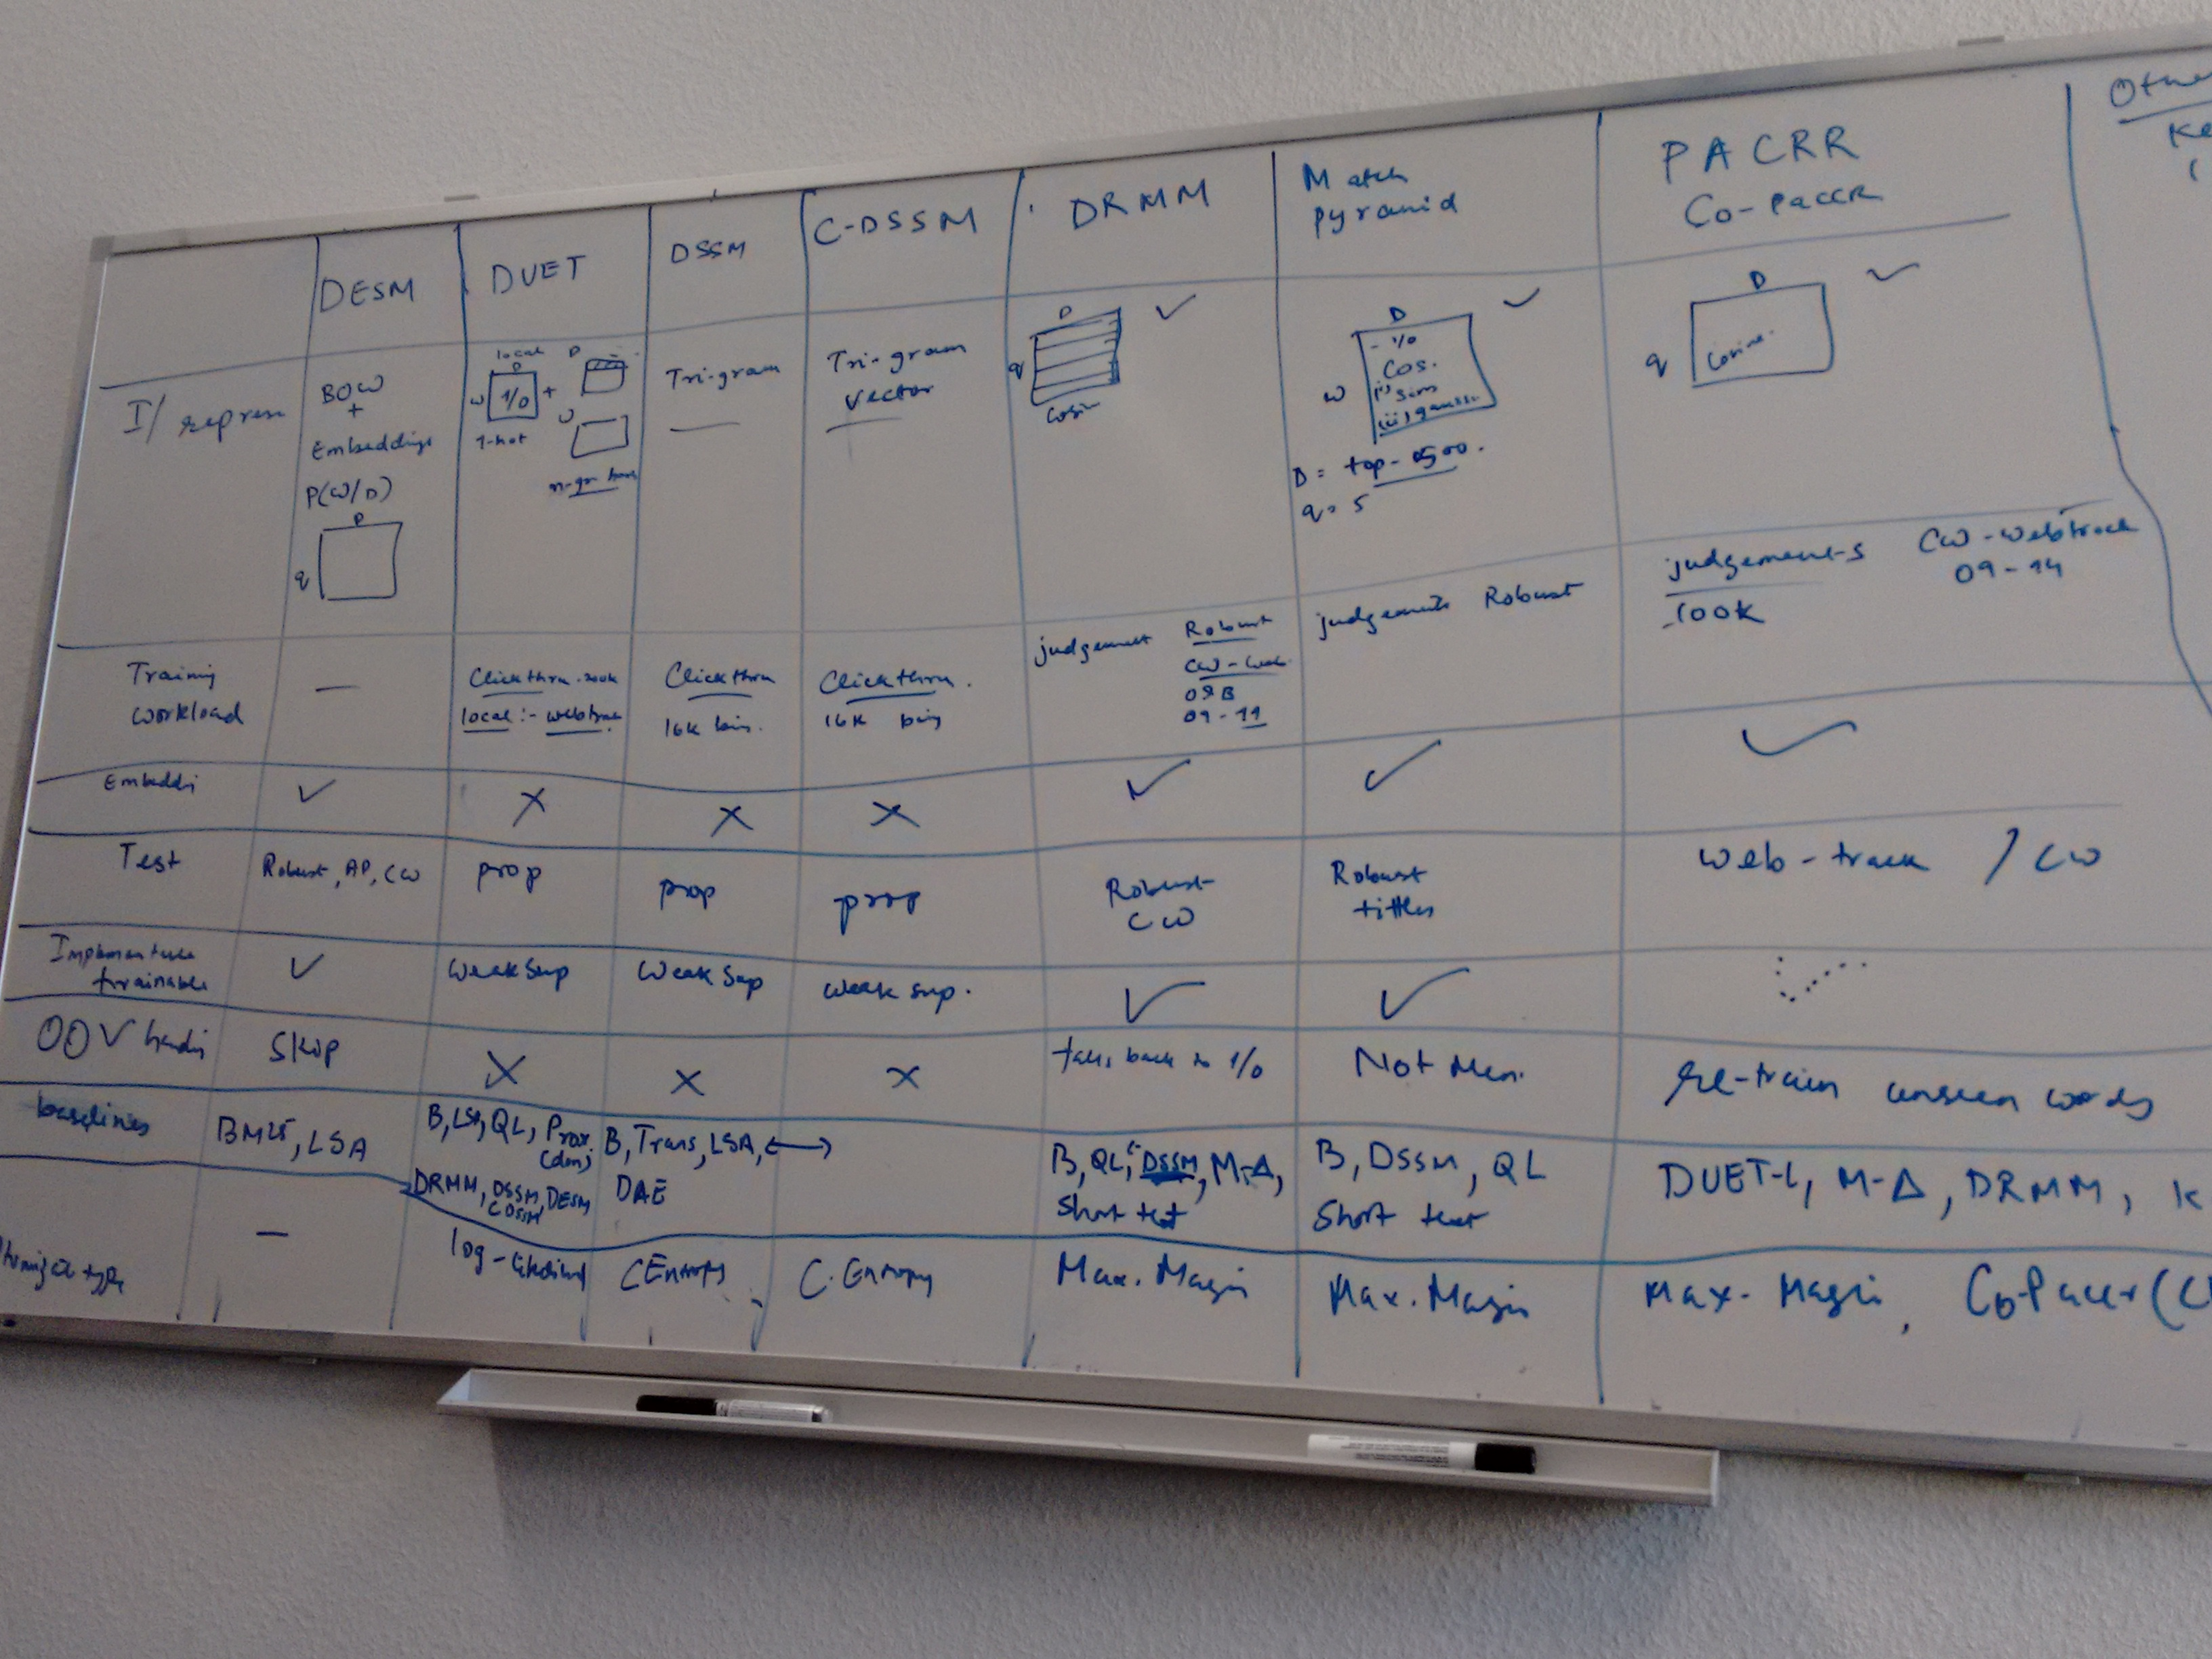
\includegraphics[width=\textwidth]{Figures/model_compare.jpg}
%     \caption{Comparison of model architectures.}
%     \label{fig:models_comparison}
% \end{figure*}

\section{Interpretability in ML}
\label{sec:interpretability_ml}

There are two main approaches to interpretability in machine learning models: {\it model agnostic} and {\it model introspective} approaches. Model agnostic approaches \citep{Ribeiro16, Ribeiro18} generate post-hoc explanations for the original model by treating it as a black box by learning an interpretable model on the output of the model or by perturbing the inputs or both. Model introspective approaches on one hand include ``interpretable'' models such as decision trees \citep{letham2015}, attention-based networks \citep{Xu2015}, and sparse linear models \citep{Ustun2016} where there is a possibility to inspect individual model components (path in a decision tree, feature weights in linear models) to generate useful explanations. On the other hand, there are gradient-based methods like \cite{Simonyan2013DeepIC} that generates attributions by considering the partial derivative of the output with respect to the input features. Following this, there were many works \citep{Lundberg17, ShrikumarGK17, Bach15, Arras17} that generate attributions by inspecting the neural network architectures.  

\subsection{Interpretability in Ranking Models}
\label{sec:interpretability_in_ir}

Recently there have been few works focused on interpretability \citep{Singh19} and diagnosis of neural IR models \citep{Rennings19, PangLG0C17, Cohen18}. In the diagnostic approaches, they use the formal retrieval constraints (``axioms'') defined for traditional retrieval models to find the differences between neural IR and learning-to-rank approaches with hand-crafted features through a manual error analysis \citep{PangLG0C17} or build diagnostic datasets based on the axioms to empirically analyse these models \citep{Rennings19}. Also, in~\cite{Cohen18} they take a diagnostic approach by probing neural retrieval models by taking each layers weights and using it as an input to a classifier for different types of NLP tasks (sentiment analysis, POS tagging, etc.). The performance on those tasks would provide insight into the type of information encoded in each layer. 

Whereas, in \cite{Singh19} they built a \textsf{Explainable Search System} (EXS) that adapts a local model agnostic interpretability approach (LIME)~\citep{Ribeiro16} to explain the relevance of a document for a query for various neural IR models (DESM, DRMM). They provide visual explanations that also helps answer why one document is ranked higher than another or what is the intent of the query according to the neural ranker. 
 
\chapter{Background} % Main chapter title

\label{Chapter3} % Change X to a consecutive number; for referencing this chapter elsewhere, use \ref{ChapterX}

\lhead{Chapter 3. \emph{Background}} % Change X to a consecutive number; this is for the header on each page - perhaps a shortened title

%-----------------------------------------------------
%	SECTION 1
%-----------------------------------------------------

In this chapter, we describe the building blocks that are commonly used to design neural network architectures for IR on which we carry out various reproducibility experiments as detailed in chapter~\ref{Chapter4}. We first describe the common input text representations that are commonly used by the existing neural IR models in section~\ref{sec:nn_input_text_repr}. Then, in section~\ref{sec:popular_architectures_for_ir} we describe a few standard neural network architectures that are commonly used in IR using the categories described in~\cite{mitra18_nir_intro}. Then we cover the different learning objectives and training strategies employed to effectively train these neural ranking models in section~\ref{sec:nn_model_learning}.

In the last section, we detail the two interpretability approaches--LIME (section~\ref{sec:lime_approach}) and DeepSHAP (section~\ref{sec:deepshap_approach}) that is used in this thesis to help understand the ranking decisions made by various neural IR models. 

\section{Input Text Representations}
\label{sec:nn_input_text_repr}

Neural IR models that learn representations of text, take raw text as input. Commonly used input text representations for neural network models in IR are pre-trained embeddings~\citep{Guo2016, matchpyramid16} or one-hot representations of terms or character n-graphs~\citep{dssm13, Mitra2017a}. Few models also take dense representations of longer chunks of text by aggregating the term pre-trained embeddings either by concatenating or taking a weighted sum over all the terms~\citep{Dehghani_sigir17}. These pre-trained embeddings can also be fine-tuned while training the neural models by directly optimizing it for the IR task of matching query-document pair~\citep{KNRM17}. Learning the term embeddings end-to-end with model training helps learn soft matching patterns that can help separate relevant from irrelevant documents but this requires large amount of training data, such as, click-through data from commercial search engines or weak supervision~\citep{Dehghani_sigir17} to learn effective representations. The pre-trained embeddings are generally learnt in an unsupervised manner either using an external large corpus or the target corpus itself using neural term embeddings models, such as,  \texttt{word2vec} (CBOW or skip-gram)~\citep{Mikolov2013} or \texttt{glove}~\citep{pennington2014glove}.

\textbf{word2vec} It consists of two architectures--\textsf{skip-gram} architecture that consists of one hidden layer with both input and output as one-hot term vectors and the model is trained by minimizing the error in predicting a term given one of its neighbouring terms defined by a context window; and \textsf{Continuous Bag-Of-Words} (CBOW) which is similar to skip-gram but the task it to minimize the error in predicting the middle term given a bag-of-words representation of all its neighbouring terms in a window. 

\textbf{Glove} It combines global and local context in the learning of embeddings by using a training objective that tries to minimize the squared difference between the dot product of the word vectors of term-neighbour pairs and the logarithm of the word's probability of co-occurrence in the corpus.

\section{Popular Architectures for IR}
\label{sec:popular_architectures_for_ir}

\subsection{Shift invariant neural operations}
Shift invariant comprises of \textit{convolutional} and \textit{recurrent} architectures. The key intuition behind these architectures, is that, the meaning of an English sentence in most cases should be consistent irrespective of the location in the document where it appears.

In shift neural operations fundamentally employ a window-based approach over the input space. A fixed size window is moved over the input space with fixed stride in each step. A typically parameterised function - called a \textit{kernel}, or \textit{filter}, or \textit{cell} is applied over each instance of this window. The parameters of the cell are shared across all window instances, which implies lesser number of total parameters in the model and more supervision per parameter per training sample.

A popular cell implementation includes multiplying with a weight matrix - then the architecture is referred to as convolutional. An example of cell without parameters is \textit{pooling} - which consists of aggregating (sum or max) over all term vectors in the window. The length of the input sequence can be variable in both cases and the length of the output of convolutional or pooling layer is a function of input length. In the \textit{global pooling strategy} there is a single window which spans over the whole input--applied on top of the convolutional layer thus giving a fixed sized output for variable length input.

In convolutional or pooling each window is applied independently. While, in \textit{recurrent} architecture the cell not only considers the current input window but also the output of the previous instance of the cell as its input. Popular RNN archictectures are--Elmon network, Long Short-Term Memory (LSTM) and Gated Recurrent Unit (GRU).

One thing to consider is how the window outputs are aggregated when using convolutional or recurrent layers. Convolutional layers are followed by either pooling or fully-connected layers that perform a global aggregation over all window instances. Fully-connected layer is aware of window position, while as pooling is agnostic to it. A global max-pooling operation could be applied to a variable size input, but it is not suitable for long sequences. Most existing \textit{interaction-based} neural IR approaches in general include convolutional architectures (DUET~\citep{Mitra2017a}, MatchPyramid, MACM~\citep{Nie_sigir_2018}, Co-PACRR, Conv-KNRM), whereas a few approaches include a convolutional architecture followed by recurrent architecture that aggregates the various local signals (PACRR, DeepRank, HiNT~\citep{Fan_hint_2018}, DeepTileBars~\citep{deeptilebars_2019}).

\subsection{Auto-encoders}
The purpose of auto-encoders is to learn a compressed representation $\vec{x}\in\mathbb{R}^{k}$ from their high-dimension representation $\vec{v}\in\mathbb{R}^{K}$ where $k \ll K$. The model is trained by feeding in the high-dimensional input and reconstructing the same representation in the output layer. The model is trained by minimizing the error between the input $\vec{v}$ and the output of the decoder $\vec{v'}$. Squared loss is employed popularly.
\begin{equation}
	\mathcal{L}_{auto-encoder}(\vec{v},\vec{v'}) = \
    {\| \vec{v} - \vec{v'} \|}^2
\end{equation}

One of the earliest neural models was a deep auto-encoder trained in an unsupervised setting on an unlabeled document corpus~\citep{SALAKHUTDINOV2009}. The documents are represented as a bag of terms and uses a one-hot representation for the terms themselves--considering only the top two thousand words in the vocabulary after removing stop words. The model is pre-trained layer-by-layer and then further trained for end-to-end learning. This model generates a condensed binary vector representation of documents. Given a search query, a corresponding hash is computed and then candidate relevant documents are retrieved that match this hash vector. A standard IR model can then re-rank this candidate set of documents. One of the main drawbacks of auto-encoders is that the model is trained on document reconstruction loss which would not model the relevance signals required to match query and documents.

\subsection{Siamese networks}
These models are used for comparing short texts. It is similar to the auto-encoders architecture but it is trained on pairs of inputs. It consists of two models that project the inputs into a common embedding space (dense representation) and predefined metric (cosine, dot) is used to commute the similarity between the embedded vectors. Most of the earlier \textit{representation-based} models employ this type of network (DSSM~\citep{dssm13}, C-DSSM~\citep{Shen2014a}).

\subsection{Interaction based networks}
In Siamese networks, both the query and documents are represented using single embedded vectors. We can instead compare individual parts of the query with individual parts of the document, to aggregate a partial evidence of relevance. This is useful, when dealing with long documents--as they contain a mixture of topics, such a strategy is more effective than representing it using a low dimensional vector. In these approaches, a sliding window is moved over the query and the document text, and each instance of the window of the query is compared with each instance of the document text window. The terms within each window can be represented in different ways, like, one-hot vectors, pre-trained embeddings or embeddings that are updated during model training. A neural model like convolutional operates over the interaction matrix and aggregates evidence across all pairs of windows compared. These interaction based approaches have been explored for ranking long documents (DUET, MatchPyramid~\citep{matchpyramid16}, PACRR, Co-PACRR~\citep{pacrr17, co_pacrr_wsdm18}).

\subsection{Lexical and semantic matching networks}
Most of the previous networks focuses on learning good representations of the text. However, these representation-based models perform poorly on rare terms and search intents. Thus, approaches that also model lexical matches using deep neural networks perform better (DRMM~\citep{Guo2016}, DUET, K-NRM~\citep{KNRM17}). Neural models that focuses on lexical matching tend to have fewer parameters and can be learned effectively with smaller datasets. In recent neural IR approaches, the input representation consists of 3-dimensional tensors that includes different types of interaction matrices capturing different signals--exact or semantic (HiNT~\citep{Fan_hint_2018}, DeepTileBars), interactions between context-sensitive or context-insensitive embeddings (POSIT-DRMM~\citep{pacrr_drmm_18}), etc.

\section{Neural Model Learning}
\label{sec:nn_model_learning}
In this section, we describe the common learning objectives and training strategies that are employed by existing neural ranking approaches.

\subsection{Learning objectives}
Similar to learning-to-rank (LTR) approaches, the learning objectives for neural IR models can be broadly categorized into--\textit{pointwise} and \textit{pairwise} ranking loss objectives.

\textbf{Pointwise Obj.} In the pointwise approach, given a query $q$ and $d \in D$ belonging to the ideal ranking set from the training dataset, a neural model is directly trained to estimate the relevance label $rel_q(d)$ which is generally a numerical value. The \textit{regression} squared loss defined in eq.~\ref{eq:reg_square_loss}~\citep{Dehghani_sigir17} and \textit{cross-entropy} loss defined in eq.~\ref{eq:cross_entropy_loss}~\citep{dssm13, Mitra2017a, co_pacrr_wsdm18} are the common ranking objectives used to train existing approaches.
\begin{equation}\label{eq:reg_square_loss}
    \mathcal{L}_{squared} = ||rel_q(d) - s(q,d)||^2\\
\end{equation}
where $s(q, d)$ is the score predicted by the model.
\begin{equation}\label{eq:cross_entropy_loss}
    \mathcal{L}_{cross-entropy} = -log\Big(\frac{\exp (f(Q,D^+))}{\sum_{D \in N} \exp (f(Q,D))}\Big)
\end{equation}
where $D^+$ is the relevant document and $N = \{D^+\} \cup D^-$ and $D^-$ is a fixed number of randomly sampled irrelevant documents (either manually judged or picked from the rest of the collection minus the candidate documents retrieved using a first stage ranker).

\textbf{Pairwise Obj.} In this approach, given a query $q$, and documents ($d^+, d^-$) where $d^+$ is ranked higher than $d^-$ with respect to the query, the neural ranking model is directly trained to learn the preference pairs or ranking between pairs of documents with respect to individual queries. The \textit{max-margin} pairwise ranking loss is the most common ranking objective (eq.~\ref{eq:max_margin_loss}) employed by numerous neural IR models~\citep{Guo2016, KNRM17, matchpyramid16}.
\begin{equation}\label{eq:max_margin_loss}
    \mathcal{L}_{max-margin} = max(0, 1 - (s(q, d^+) - s(q,d^-))
\end{equation}
where s(q, d) is the score returned by the neural ranking model.

\subsection{Training strategies}
\textit{Supervised learning} is the most common strategy employed by the existing approaches where query-document pair labels are available. The labels are available either through relevance judgements from popular TREC ad-hoc tasks or through implicit feedback from user interactions with commercial search engines (click-through) data. 

\textit{Weakly supervised learning} As neural models require large amounts of data, and since annotated data is limited, in this learning strategy query-document labels are generated using an existing traditional IR model (BM25, QL) that gives pseudo labels. Most recently,~\cite{Dehghani_sigir17} proposed to train a neural ranking model with weak supervision and show that it provides upto 35\% improvement over the BM25 baseline that is used as the weak ranker or annotator.

\textit{Semi-supervised learning} In this approach, a small set of high quality manually judged query-document pairs are used along with large sets of unlabeled or pseudo-labeled data. For neural models, fine-tuning weak supervision trained models using a small set of labeled data is shown in~\citep{dehghani2018fidelityweighted}. Recently, \cite{Bo_coling18} proposed a neural model with a joint supervised and unsupervised loss objectives. The learned representation is optimized for the context of IR by minimizing a supervised loss that accounts for errors in query-document relevance matching, and a unsupervised loss that computes the document reconstruction loss (e.g. auto-encoders). They show that neural IR models jointly learnt from labeled and unlabeled data benefit from both the generic semantics in unlabeled data and target-specific features in labeled data.

\section{Interpretability Approaches}
In this section, we describe in detail two interpretability approaches--one that is \textit{model-agnostic} (LIME) and the other a \textit{model-introspective} (DeepSHAP) that we use in this thesis to understand the decisions made by various neural IR models (such as, exactly \textit{why} a particular document is relevant to a given query for this model). The approach of how these interpretability methods are modified or applied to the context of IR is described in Chapter~\ref{Chapter5}.

\subsection{Local Interpretable Model-Agnostic Explanations}\label{sec:lime_approach}

Local interpretable model-agnostic models (LIME)~\citep{Ribeiro16, Ribeiro18} are used to explain individual predictions by approximating the local behavior of complex black-box models. The important characteristics underlying LIME is that the explanation model needs to be (1) \textit{interpretable}, (2) \textit{locally faithful} and (3) \textit{model-agnostic} which~\cite{Ribeiro16} respectively define as (1) ``provide qualitative understanding between the input variables and the response'', (2) the explanation ``must correspond to how the model behaves in the vicinity of the instance being predicted'' and (3) ``the explanation should
be able to explain any model''. The explanations are created using ``interpretable'' models (e.g. sparse linear models) trained on interpretable feature representations. The training data is sampled from perturbing the instance to be explained weighted by its proximity to that instance and the corresponding predictions obtained from the black box model.

Approaches in this space tend to differ based on the type of black-box model (classification, regression), the interpretable feature space and the definition of locality. For example, the interpretable feature space for text based models is the space of all words in that instance represented using one-hot vectors even if the black-box model uses word embeddings. The explanation then is a visualization of the simple model depending on the context and the model itself.

LIME is an approach designed specifically to explain the output of a classifier. To illustrate their approach, consider a trained binary classifier $\mathcal{B}$ and an instance document to classify $d$. Assume that $\mathcal{B}$(d) is a probability distribution across the classes. The objective of LIME is to train a simple model $\mathcal{M}_d$ that minimizes $\mathcal{L}$($\mathcal{B}$, $\mathcal{M}_d$, $\pi_d$) which is a measure of how far $\mathcal{M}_d$ is in approximating $\mathcal{B}$ in the locality defined by $\pi_d$ which is a proximity measure between the perturbed instance and the instance to be explained. The explanation $\xi(x)$ produced by LIME can be obtained using the following equation.
\begin{equation}
    \xi(x) = \underset{g\in G}{\arg\min}\  \mathcal{L}(\mathcal{B}, \mathcal{M}_d, \pi_d) + \Omega(g)
\end{equation}
G is the family of explanation models (e.g. all possible linear regression models). $\Omega(g)$ is the complexity measure of the explanation model $g$. For example, for linear models, $\Omega(g)$ could be the number of non-zero weights. The loss $\mathcal{L}$ to be reduced is the dissonance between the simple $\mathcal{M}_d$'s predictions and the labels produced by $\mathcal{B}$ for all $d'\in \pi_d$ . 

For the case of explaining text based models, $\mathcal{M}_d$ is a sparse linear regression model (\textit{ridge regression}\footnote{\url{https://scikit-learn.org/stable/modules/generated/sklearn.linear_model.Ridge.html}}) trained on a bag of words feature space. $d' \in \pi_d$ is generated by perturbing document $d$. In LIME, $d'$ is created by removing random words from random positions in d. The locally weighted squared loss $\mathcal{L}$ of the sparse linear model is as defined in eq.~\ref{ridge_loss}, where $\pi_d$ is an exponential kernel on some distance function \textit{dist} (e.g. cosine distance for text) given in eq.~\ref{exp_kernel}.
\begin{equation}\label{ridge_loss}
    \mathcal{L}(\mathcal{B}, \mathcal{M}_d, \pi_d) = \underset{d, d' \in D}{\sum} \pi_d(d')(\mathcal{B}(d) - \mathcal{M}_d(d'))^2
\end{equation}
\begin{equation}\label{exp_kernel}
    \pi_d(d') = exp(\frac{-dist(d, d')}{\sigma^2})
\end{equation}
The coefficients of the features of the trained $\mathcal{M}_d$ indicates the importance of the words for that instance. Features with highest positive coefficients are assumed to be important for the model to classify the instance to the predicted class, where as those with highest negative coefficients are assumed to work for the different class. Limiting the number of words returned for the explanation is chosen based on feature-selection strategies, such as, LASSO (using the regularization parameter $\lambda$), or forward and backward selection of features.
%Obtaining a label (probability distribution across classes here) for a perturbed instance is straightforward for a classifier whereas for ranking models this is tricky.

\subsection{DeepSHAP}\label{sec:deepshap_approach}
DeepSHAP~\citep{Lundberg17} is one of the popular \textit{model-introspective} approaches that enables us to understand the predictions of complex deep-learning models. It produces explanations by using the input feature attributions for a given instance and the prediction of the model for that instance. DeepSHAP is a modification of the DeepLift~\citep{ShrikumarGK17} algorithm to efficiently estimate the shapley values over the input feature space for a given instance. The shapley value is a term coined by Shapley~\citep{shapley1953value} in cooperative game theory to refer to the contribution of a feature in a prediction. More specifically, shapley values explain the contribution of an input feature towards the \emph{difference} in the prediction made vs the average prediction value.

DeepLIFT explains the difference in output or prediction from some `reference' output with respect to the difference of the input (to explain) from a `reference' input. DeepLIFT uses a `\textbf{summation-to-delta}' property that states that:
\begin{equation}\label{eq:sum_to_delta}
    \overset{n}{\underset{i=1}{\sum}}C_{\Delta x_i \Delta t} = \Delta t
\end{equation}
where $t=f(x)$ is model output, $\Delta t=f(x) - f(r)$, $\Delta x_i= x_i - r_i$ and $r$ is the reference input. It can be described as the amount difference-from-reference of the output that is attributed to the amount of difference-from-reference of the input. The authors define a function (eq.~\ref{eq:deeplift_multiplier}) analogous to partial derivatives to compute the feature importance scores and use the chain rule to backpropagate the activation differences from the output layer to the original input.
\begin{equation}\label{eq:deeplift_multiplier}
    m_{\Delta x \Delta t} = \frac{C_{\Delta x \Delta t}}{\Delta x}
\end{equation}
The choice of reference input depends on domain specific knowledge; For example, in digit classification task on the MNIST dataset, they use a reference input of all-zeros as that is the background of the images. For object detection in images, a plain black image is often used.
\chapter{Reproducibility of Neural IR models} % Main chapter title

\label{Chapter4} % Change X to a consecutive number; for referencing this chapter elsewhere, use \ref{ChapterX}

\lhead{Chapter 4. \emph{Neural IR models Reproducibility}} % Change X to a consecutive number; this is for the header on each page - perhaps a shortened title
In this chapter, we will discuss in detail the architectures of various deep learning IR models that we selected to reproduce along with the experimental setup, implementations and the discussion of the results we obtained. We initially implemented two \textit{interaction-based} models--DRMM~\citep{Guo2016} and MatchPyramid~\citep{matchpyramid16}, as it was shown that \textit{interaction-based} approaches clearly outperform \textit{representation-based} approaches in terms of retrieval effectiveness in a recent empirical study~\citep{Nie_ictir18}. We selected DRMM as it is shown to outperform strong IR baselines and other recent deep learning based approaches~\citep{Onal_NIR2018}. 

As DRMM doesn't consider the contexts in which terms occur, we considered \textit{position-aware} approaches such as MatchPyramid that mimics image recognition for text matching and a \textit{position-aware} extension of DRMM using PACRR like \textit{n-gram} matching features to give PACRR-DRMM~\citep{pacrr_drmm_18}. We then implement a model NPRF-DRMM that uses the recently proposed generic neural pseudo relevance feedback (NPRF) framework~\citep{li2018nprf} that enables the use of PRF along with state-of-the-art neural IR models by embedding them as building blocks. The proposed framework can use existing neural IR models by using them as scorers in evaluating the relevance of a document relative to the top-ranked documents and to the query without modifying their architectures. 

All the reproducibility experiments are carried out on the TREC Robust04 benchmark dataset for ad-hoc retrieval. The dataset contains 528,155 documents (TREC disks 4 \& 5 minus Congressional Records) and 250 queries that is used in the TREC 2004 Robust track~\citep{robust04}. Manual high-quality relevance judgements are available for all queries, where both relevant and non-relevant documents are marked. Statistics of the collection are included in Table~\ref{tab:trec_robust04_stats}.

\begin{table}[]
    \centering
    \begin{tabular}{cccc}
    \toprule
        \#Vocabulary & \#Document & Avg Doc. Len. & \#Query \\
        \midrule
        0.6M & 528K & 477 & 250\\
    \bottomrule
    \end{tabular}
    \caption{Statistics of the TREC Robust04 collection }
    \label{tab:trec_robust04_stats}
\end{table}

%-----------------------------------------------------
%	SECTION 1
%-----------------------------------------------------
\section{Deep Relevance Matching Model (DRMM)}
The deep relevance matching model (DRMM) for ad-hoc retrieval is an interaction-focused model that uses a joint deep architecture at the query term level for relevance matching~\citep{Guo2016}. First, they build local interactions between each pair of terms from a query and a document based on cosine similarity of term embeddings. Then for each query term, they map the variable length local interactions into a fixed-length matching histogram. Based on this matching histogram, they employ a feed forward matching network that learns hierarchical matching patterns and produces a matching score. Finally, the overall matching score is computed by aggregating the individual query term matching scores using a term gating network. The model architecture is depicted in Figure~\ref{fig:drrm_architecture}.
\begin{figure*}
    \centering
    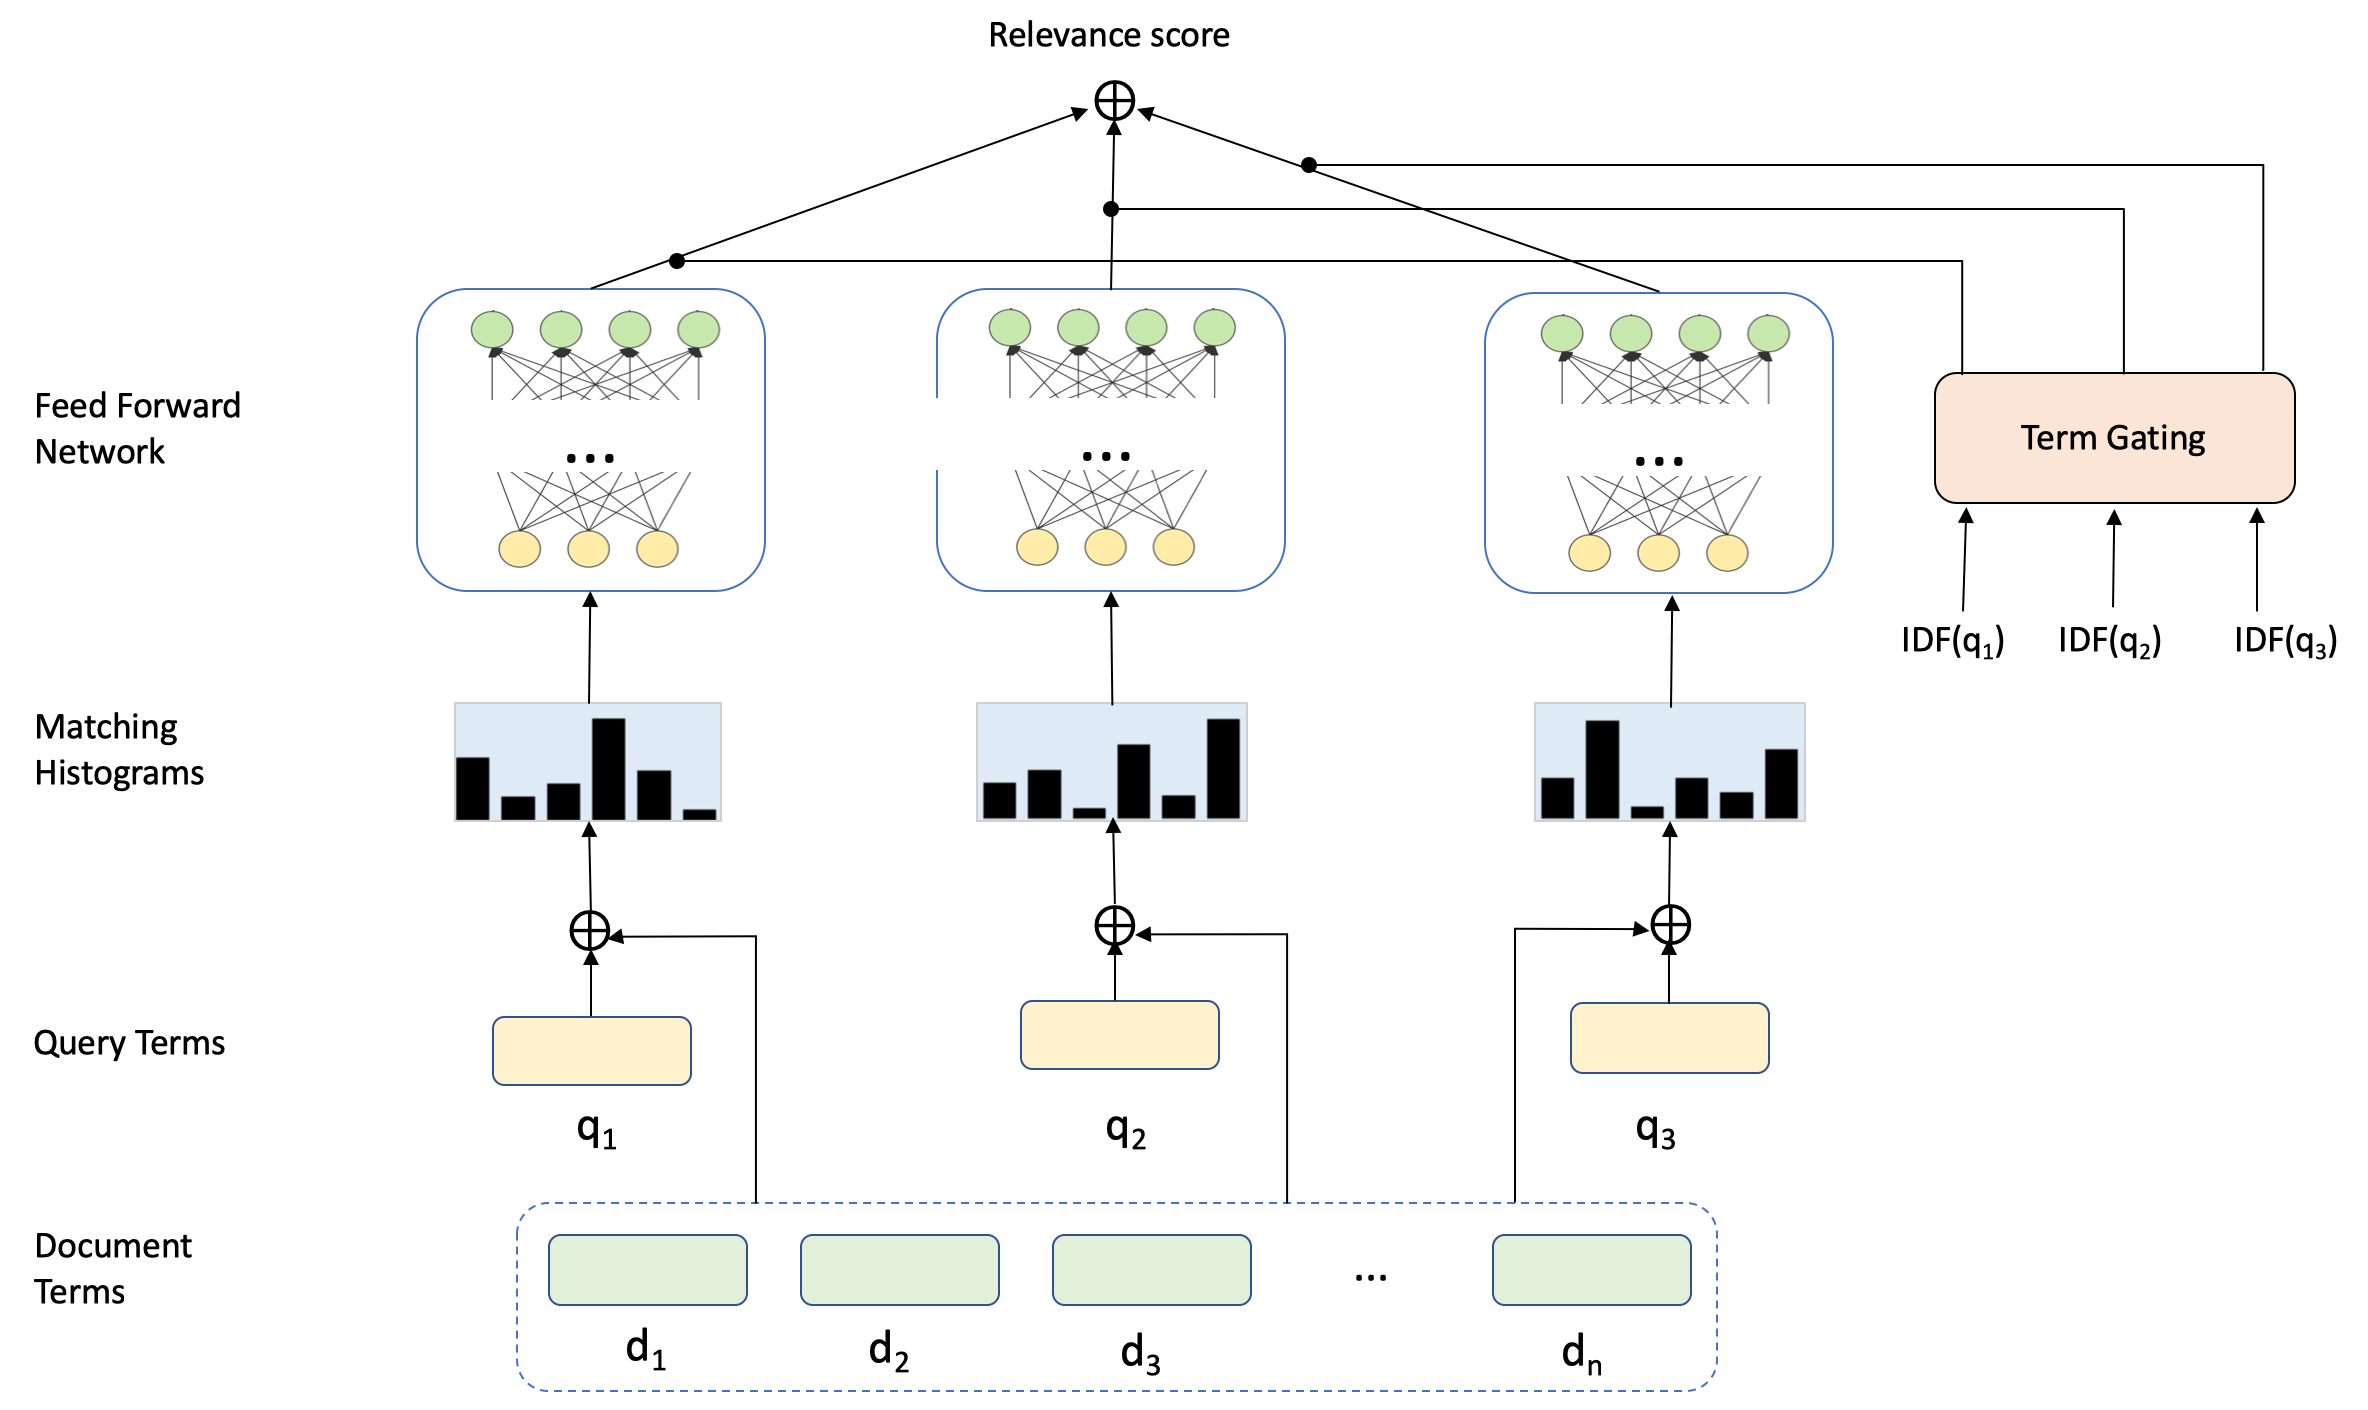
\includegraphics[width=15cm]{Figures/drmm_ppt.png}
    \caption{Deep Relevance Matching Model (DRMM) architecture}
    \label{fig:drrm_architecture}
\end{figure*}

Formally, both query and documents are represented using a set of term vectors denoted by $q=\{w^{(q)}_1,...,w^{(q)}_M\}$ and $d=\{w^{(d)}_1,...,w^{(d)}_N\}$, and $s$ denotes the final relevance score, then we have
\begin{align*}
    z^{(0)}_i &= h(w^{(q)}_i \otimes d), & i=1,....,M \\
    z^{(l)}_i &= \tanh(W^{(l)}z^{(l-1)}_i + b^{(l)}), & i=1,...,M,\ l=1,...,L \\
    s &= \sum_{i=1}^{M} g_i z^{(L)}_i &
\end{align*}
where $\otimes$ denotes the interaction operator (cosine similarity) between a query term and the document terms, $h$ is the mapping function to get matching histograms, $z^{(l)}_i$ denotes the intermediate hidden layers for the $i$-th query term, and $g_i$ denotes the aggregation weight from the term gating network.

\textbf{Matching Histogram Mapping}. Since the local interactions is within the interval [-1, 1], the histogram is obtained by discretizing the interval into a set of ordered bins and accumulating the count of local interactions for each bin. In this work, fixed size bins are used and the exact matching signal is treated as a separate bin. They explore three different ways of mapping:
\begin{description}
    \item[\normalfont\itshape Count-based Histogram (CH):] Takes the count of interactions in each bin as the histogram value.
    \item[\normalfont\itshape Normalized Histogram (NH):] Normalize the count value in each bin by the total count, to focus on relative rather than absolute number of different levels of interaction.
    \item[\normalfont\itshape LogCount-based Histogram (LCH):] Takes the logarithm over the count value in each bin, to reduce the range.
\end{description}

% \textbf{Feed forward Matching Network}. The matching histogram is used as input to a feed forward matching network to learn the hierarchical matching patterns and to produce a matching score for each query term. 

\textbf{Term Gating Network}. The model explicitly models query term importance using a term gating network to get a aggregation weight for each term. The softmax function is used as the gating function.
\begin{align*}
    \centering
    g_i &= \frac{\exp (w_g x^{(q)}_i)}{\sum_{j=1}^{M} \exp (w_g x^{(q)}_j)}, & i=1,...,M
\end{align*}
where $w_g$ is the weight vector of the gating network. Two different inputs were considered: \textit{term vector}, where query term vectors are used; \textit{inverse document frequency (IDF)}, where the IDF of the query term is used.

\textbf{Model Training}. The model is trained on triples ($q, d^+, d^-$), where document $d^+$ is ranked higher than document $d^-$ with respect to $q$, minimizing pairwise max-margin loss as in eq.~\ref{eq:drrm_loss_objective}.

\begin{equation}\label{eq:drrm_loss_objective}
    \mathcal{L}(q,d^+,d^-;\Theta) = \
    {\max (0, 1 - s(q,d^+) + s(q,d^-))}
\end{equation}
where $s(q,d)$ denotes the predicted matching score and $\Theta$ are the parameters of the feed forward network and term gating network. The stochastic gradient descent method \textsf{Adam} with mini-batches (20) is used to trained the model.

% \textbf{Datasets}. Experiments are run using two TREC collections Robust04 and ClueWeb-09-Cat-B. Topics are accumulated from TREC Web Tracks 2009, 2010, and 2011. ClueWeb-09-Cat-B is filtered to the set of documents with spam scores in the $60^{th}$ percentile, using the Waterloo fusion spam scores. For both datasets, both the title and description of the TREC topics are used. The retrieval experiments are conducted using the Galago search engine.

\subsection{Experimental Setup}\label{drmm_exp_setup}
We use the \textit{title} of each TREC topic as queries in our experiments. The indexing and retrieval is implemented using Lucene\footnote{\url{https://lucene.apache.org/}}. During indexing and retrieval, both document and query words are white-spaced tokenized, lower-cased and stemmed using Krovetz stemmer available here\footnote{\url{https://github.com/rmit-ir/KrovetzStemmer}}. Stopword removal is performed on the query words during retrieval from the Lucene index based on a custom stopwords list\footnote{See Lucene \textsf{EnglishAnalyzer} for details.}. We compare the DRMM model retrieval performance against the BM25 baseline using the default parameters (\textit{k1}:1.2 and \textit{b}:0.75) from Lucene.

%\paragraph{Term Embeddings}
\textbf{Term Embeddings}. The 300 dimensional vectors used as term embedding input for DRMM are trained using CBOW model~\citep{Mikolov2013} on Robust04 collection. The parameters used are context window size (10), negative samples (10) and subsampling of frequent words with a threshold of $10^{-4}$ using \texttt{word2vec}\footnote{\url{https://radimrehurek.com/gensim/models/word2vec.html}}. The corpus is preprocessed removing HTML tags, stemming using Krovetz stemmer and stopword removal using NLTK\footnote{\url{https://www.nltk.org/}}. We discarded from the vocabulary terms that occur less than 10 times in the collection resulting in a vocabulary of size 106K. The out-of-vocabulary (OOV) terms are ignored while preparing the model input.

\textbf{Model Implementation}. We implemented the DRMM model using the Keras functional api\footnote{\url{https://keras.io/getting-started/functional-api-guide/}} with a Tensorflow backend. The network configuration of the DRMM model is set as: one histogram layer (30 nodes), two hidden layers in the feed forward matching network (5 and 1 nodes) and 1 output layer with the term gating network for the final relevance score as suggested in the paper based on hyperparameter tuning on the validation set. We implement the variant DRMM\textsubscript{\textit{LCH}x\textit{IDF}} that uses \textit{logcount-based} histogram as input and \textit{term vector} for computing query term importance in the term gating network. We use a step-decay adaptive learning rate that drops the learning rate by a factor of 0.9 every 10 iterations (initial learning rate=0.001). We train the model for 100 iterations, where in each iteration the model trains on 1000 mini-batches (20). Thus, the model would train on roughly 2M training pairs of data. The training pairs for each mini-batch is randomly sampled from all possible pairs of relevant and irrelevant documents from the relevance judgements for the queries in the training set. 

\textbf{Evaluation}. We conduct 5 fold cross-validation to minimize overfitting due to the limited number of queries in the collection. Topics are randomly split into 5 folds and the parameters are tuned on 4-of-5 folds. The retrieval performance is evaluated on the final fold in each case using the optimal parameters. This process is repeated 5 times, once for each fold. Mean Average Precision (MAP) is the metric that is optimized for during training. We use a re-ranking strategy for evaluation, where first we retrieve the top-2000 documents using BM25 model and then re-rank it using the neural model to obtain the top-1000 documents that are used to compute the evaluation metrics. Each displayed metric is the average of the five 5-fold evaluation values.

\begin{table}[]
    \centering
    \begin{tabular}{lccc}
    \toprule
        Model Name & MAP & nDCG@20 & P@20 \\
        \midrule
        BM25 & 0.2405 & 0.4038 & 0.347 \\
        DRMM\textsubscript{\textit{LCH}x\textit{IDF}} & 0.257 & 0.4103 & 0.352 \\
        DRMM\textsubscript{\textit{LCH}x\textit{IDF}} \textit{paper} & 0.268 & 0.423 & 0.381\\
    \bottomrule
    \end{tabular}
    \caption{DRMM Model retrieval performance on the Robust04 collection}
    \label{tab:drmm_eval}
\end{table}

\subsection{Results and Discussion}
We observe from Table~\ref{tab:drmm_eval} that our implementation of DRMM provides improvements over the BM25 baseline across all evaluation metrics. However, this implementation gives results lower than that from the paper because of the following reasons: due to different random partitions of the data, and in the original paper they re-rank the top documents returned from a well-tuned query-likelihood (QL) model. Also, they use a different sampling strategy to generate the training pair instances since there is a data imbalance problem, where the pairs available for each query are significantly different (i.e. some queries have more positive samples than others). Then, the model could be dominated by a few queries leading to lower performance. 

We also empirically observe that using word embeddings not trained on the collection, such as, \texttt{word2vec}\footnote{\url{https://code.google.com/archive/p/word2vec/}} or \texttt{glove}\footnote{\url{https://nlp.stanford.edu/projects/glove/}} embeddings results in lower performance over the evaluation metrics. This is because the coverage of these term embeddings are only 35\% and 50\% of the 0.1M vocabulary using \texttt{word2vec} and \texttt{glove} respectively. The filtering of the vocabulary size from 0.6M to 0.1M by removing words that occur less than 10 times in the collection is a very important preprocessing step in effectively training a DRMM model that is better than the baseline. This is because there isn't sufficient data to learn reliable term embeddings for the words that occur less than 10 times in the collection. 

%-----------------------------------------------------
%	SECTION 2
%-----------------------------------------------------
\section{MatchPyramid for ad-hoc retrieval}

The MatchPyramid model for ad-hoc retrieval~\citep{matchpyramid16} is an interaction-focused model that first builds a matching matrix from the local interactions between the terms from query and document using word embeddings. 
%This model uses pretrained word embeddings to first create a query-document term interaction matrix, where each element is the cosine similarity between the query term and document term. 
This matching matrix is then viewed as an image and fed into a 2D convolutional neural network (CNN) to extract hierarchical matching patterns. Finally the matching patterns from the CNN are fed into a multi-layer perceptron (MLP) to aggregate a relevance score. The model is known to capture different matching patterns, such as, n-grams and un-ordered n-terms. The model architecture is shown in Figure~\ref{fig:matchpyramid_architecture}. %The `OOV' token is represented by an all-zeros embedding vector that is used for padding the input interaction matrix.
\begin{figure*}
    \centering
    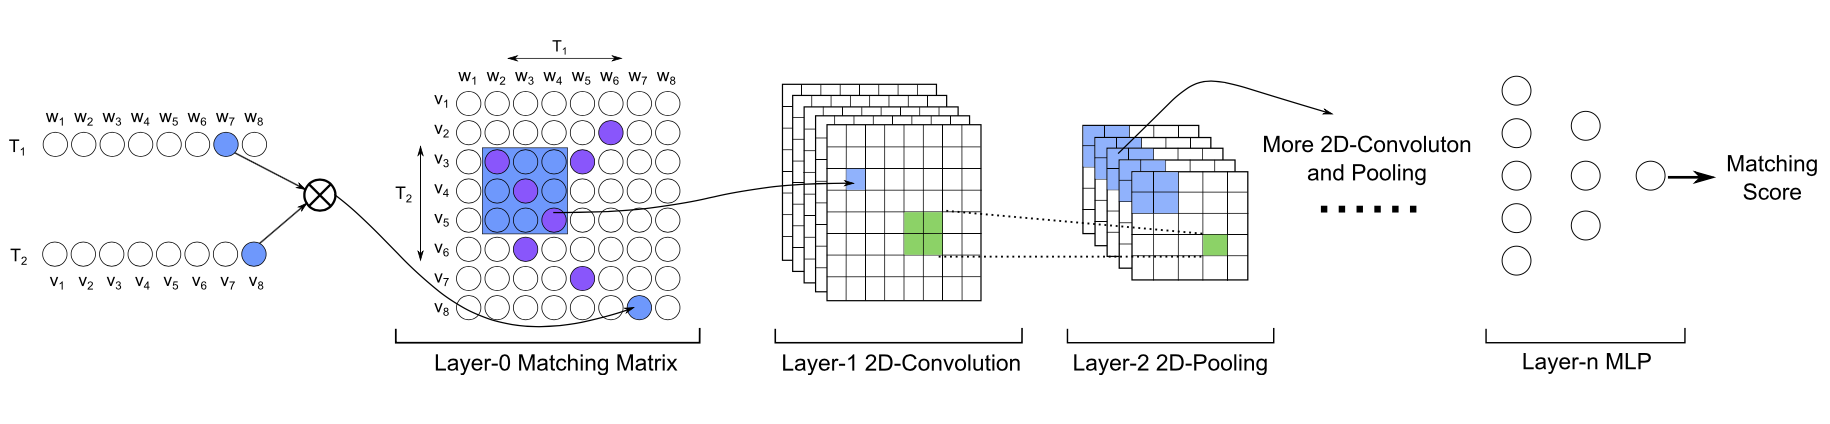
\includegraphics[width=\textwidth]{Figures/MATCHPYRAMID.png}
    \caption{MatchPyramid architecture~\citep{matchpyramid16}}
    \label{fig:matchpyramid_architecture}
\end{figure*}

\textbf{Matching Matrix}. It is a two-dimensional matrix where each element \textbf{M}\textsubscript{ij} denotes the similarity between the \textit{i}-th word $w_i$ in the query and the \textit{j}-th word $v_j$ in the document. The order in which the words appear is preserved while creating the matrix. They define four different similarity functions based on the words $w_i$ , $v_j$ or their corresponding embeddings: \textit{indicator function} (MP-Ind)--checks if two words are identical; \textit{cosine similarity} (MP-Cos)--between the word embeddings; \textit{dot product} (MP-Dot); \textit{gaussian kernel} (MP-Gau)--as defined in eq.~\ref{eq:mp_gau_kernel}.
\begin{equation}\label{eq:mp_gau_kernel}
    \mathbf{M}_{ij} = \
    e^{{-||\vec{w_i} - \vec{v_j}||}^{2}}
\end{equation}

\textbf{Hierarchical Convolution}. This consists of convolutional and dynamic pooling layers which are commonly used in CNN. The kernel sizes in each convolutional layer determines the maximum size of n-gram features that we take into account. And the pooling layer determines the most important information that needs to be selected from the convolutional layer. This is useful especially when we consider documents that have hundreds of words of which most are background words.

\textbf{Training Objective}. They use a pairwise ranking loss such as hinge loss with a margin of 1.0 for training the MatchPyramid model similar to the objective defined in eq.~\ref{eq:drrm_loss_objective} for the DRMM model.

\subsection{Experimental Setup}
The indexing and retrieval experimental setup for the TREC Robust04 collection is the same as described in section~\ref{drmm_exp_setup}. The term embeddings used for all the models are the \textit{glove} embeddings of 50 dimensions which are obtained by training on the Wikipedia corpus. We follow the exact same evaluation method as described for the DRMM model (section \ref{drmm_exp_setup}) here.

\textbf{Model Implementation}. We implement the model variants MP-Ind and MP-Cos using Keras. The optimization method \texttt{Adam} with mini-batches (32) is used for model training. The initial learning rate is set to $10^{-4}$ and uses a step-decay learning rate schedule that drops the learning rate by a factor of 0.9 after every 10 epochs. The network configurations for the MatchPyramid models are selected based on MAP on the validation set. We use one convolutional layer with kernel size 3 x 3 and feature maps set to 8, one dynamic pooling layer with pooling size 2 x 10, and two fully connected layers (128 nodes and 1 node respectively) with ReLU as the activation as suggested in~\citep{matchpyramid16}. We use one hierarchical convolution layer as more layers will lead to overfitting due to limited data. In our experiments, the maximum query length is set to 5 and the maximum document length is set to 500.

\begin{table}[]
    \centering
    \begin{tabular}{lccc}
    \toprule
        Model Name & MAP & nDCG@20 & P@20 \\
        \midrule
        BM25 & 0.2405 & 0.4038 & 0.347 \\
        MP-Ind & 0.1823 & 0.3353 & 0.286 \\
        MP-Ind \textit{paper} & 0.169 & 0.319 & 0.281 \\
        MP-Cos & 0.1898 & 0.3328 & 0.276\\
        MP-Cos \textit{paper} & 0.189 & 0.330 & 0.290\\
    \bottomrule
    \end{tabular}
    \caption{MatchPyramid models retrieval performance on the Robust04 collection}
    \label{tab:mp_eval}
\end{table}

\subsection{Results and Discussion}
When we look at Table~\ref{tab:mp_eval} we see that the MatchPyramid models cannot compete with the BM25 retrieval baseline across all measures. However, we can see that our implemented model performance is comparable to the model performance mentioned in the paper. As both MP-Ind and MP-Cos show similar performance, we can see that MP-Cos is able to encode exact matching along with semantic signals giving higher importance to exact matching over semantic similarities which is important for relevance matching. We empirically observe that it is better to use \texttt{glove} embeddings (50-dim) than the \texttt{word2vec} embeddings (300-dim) trained on the collection, this could be because the MatchPyramid models have a huge number of parameters and limited training data thus using an embedding with fewer (50) dimensions gives better performance. The best pooling size of 2 x 10 shows that it picks importance signals equivalent to the median query length on the query side, and on the document side, it aggregates importance signals from every 50 words which is close to the average length of a paragraph.

%------------------------------------------------------
%	SECTION 3
%------------------------------------------------------
\section{Deep Relevance Ranking using Enhanced Document-Query Interactions (PACRR-DRMM)}

In this paper~\citep{pacrr_drmm_18}, the focus is on enriching DRMM with context-sensitive representations of the query, as in the original model query terms are scored relative to the document terms without taking into consideration the context in which the term occurs, its akin to a Bag-of-Words (BoW) model. Whereas, the 
PACRR model~\citep{pacrr17,Yates17} is a \textit{position-aware} interaction based model that uses similarity matrices that captures semantic similarity between each query term and each individual term in the document, also preserving term order. Thus, PACRR-DRMM is an extension of DRMM, that uses the query term encodings obtained from PACRR-like convolutional \textit{n-gram} matching features as an input for the  DRMM model.

\textbf{PACRR}. The query-document similarity matrix (\textit{sim}) is created using the cosine similarity between the q-term and d-term embeddings. To keep the dimensions of the \textit{sim} fixed across queries and documents of varying length, the queries are padded to max query length $l_q$ and documents are either truncated/padded to max document length $l_d$\footnote{PACRR-\textit{firstk} as highlighted in~\citep{pacrr17}.}. Then the following pipeline is applied: 
\begin{description}[font=\normalfont\itshape]
    \item[convolutional relevance matching.]  convolutional layers of different kernel sizes $n$ x $n$ (n=2, 3,...,$l_g$) are applied on the similarity matrix to capture positional information over text windows of different lengths (\textit{n-grams}). For each kernel size, multiple kernel filters are used. The convolutional layer uses a stride (1, 1) along the query dimension and stride of (1, n) along the document dimension, so that it operates over consecutive terms that existed in the document.
    \item[max pooling layers.] First, max pooling is applied across the dimension of the filters to preserve the strongest signal from different filters. Then, row-wise \textit{k}-max pooling to capture the $k$ strongest signals for each query term and all document terms.
    \item[MLP for global relevance.] The resulting matrices are concatenated into a single matrix where each row is a document-aware query term encoding. To each row, the IDF of the query term is appended which is normalized by taking softmax with respect to the IDFs of all query terms. The rows are then concatenated to give a single vector that is used as input to a MLP~\citep{co_pacrr_wsdm18} to give a relevance score.
\end{description}

%These matrices are then fed through a series of convolutional, max-k pooling and recurrent layers to capture interactions, such as, bi-gram and tri-gram matches. In this model, convolutional layers are used to capture both unigram matching and positional information over text windows over different lengths; max-k pooling layers are along query dimension, to preserve matching signals across different query terms; recurrent layer combines signals from different query terms to produce query-document relevance score.

%The similarity between a query term and document term is calculated by taking the cosine similarity between the corresponding pre-trained word2vec vectors. Query-document similarity matrices can provide rich signals to perform n-gram matching which corresponds to consecutive document terms that are highly similar to at least one of the query terms. Since the subsequent processing in PACRR's convolutional layer requires that each query-document similarity matrix have the same dimensions, we transform the raw similarity matrices $sim_{|q|*|d|}$ to $sim_{l_q * l_d}$ matrices with uniform number of rows and columns. The query dimension $l_q$ is zero padded to the maximum query length. Two strategies were designed with respect to the document dimension $l_d$.
% \begin{itemize}
%     \item \textit{firstk} - In this the first $k$ columns/terms of the matrix are kept. If $k > |d|$ then the remaining columns are zero-padded.
%     \item \textit{kwindow} - For the case of unigrams, the top $l_d$ terms with the highest similarity to query terms are chosen. But for text snippets of length $n$, a similarity matrix $sim^n_{l_q * l_d}$ is created for each query-document pair and $n$. So $kwindow$ calculates the maximum similarity between each term in $n$ and the query terms, and then calculates the average similarity over each $n$-term window. Then the top $k$ windows based on the average similarity is selected.
% \end{itemize}

% \textbf{Convolutional relevance matching} is to match text snippets with different length from a query and a document given an query-document similarity matrix as input. Each convolutional layer is responsible for a specific n: by applying a kernel to $n * n$ windows, providing a similarity signal for each window. When \textit{firstk} method is used, each convolutional layer gets the same similarity input matrix $sim_{l_q * l_d}$ because \textit{firstk} produces same matrix irrespective of $n$. But when $kwindow$ method is applied each convolutional layer will get a similarity matrix $sim^n_{l_q * l_d}$ corresponding to the kernel $n * n$. Different convolutional layers with kernel sizes $2*2, 3*3,....,l_g*l_g$ corresponding to bi-gram, tri-gram and n-gram matchings are used. Each convolutional layer applies $n_f$ filters, $n_f$ is a hyperparameter. The convolutional layer uses a stride (1,1) along the query dimension and stride of (1,n) along the document dimension, so that it operates over consecutive terms that existed in the document.

% \textbf{Two max pooling layers} is to capture the strongest similarity signals for each query term. A small number of signals $n_s$ is used so that the model is not biased by document length. For each query term, first max-pooling is performed over the filter dimension $n_f$ to keep the strongest indicator from the different filters, as they assume that there is only a single true matching in a $n*n$ window. Then $k-max$ pooling is performed over the query dimension to keep the $n_s$ strongest signal for each query, thus producing a 3-dimension tensor $P_{l_q * l_g * n_s}$.

% \textbf{Recurrent layer for global relevance} is to transform the query term similarity signals in $P_{l_q * l_g * n_s}$ into a document relevance score. A Long Short-Term Memory (LSTM) recurrent layer is applied to $P$, taking a sequence of vectors as input and transforming it to a final relevance score. After splitting the above matrix across the query dimension, then for each query $q_i$ we have a matrix $P_{l_g*n_s}$ which is flattened into a vector by concatenating rows together and appending the normalized IDF score of $q_i$.

\begin{figure*}
    \centering
    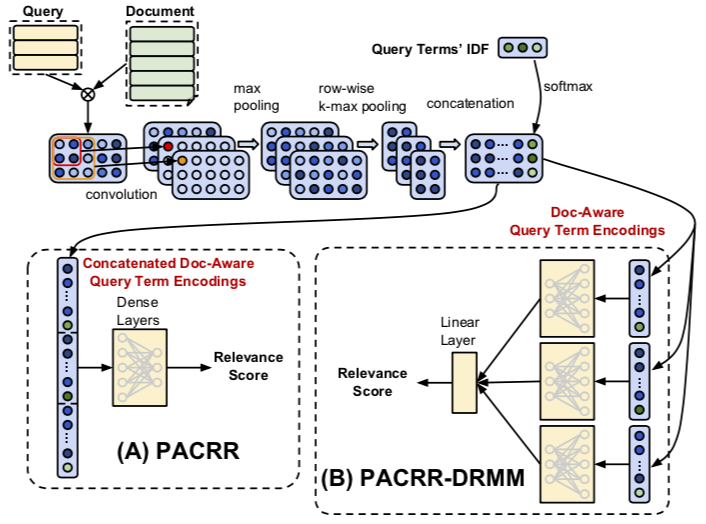
\includegraphics[width=10cm]{Figures/pacrr_drmm.png}
    \caption{PACRR-DRMM architecture~\citep{pacrr_drmm_18}}
    \label{fig:pacrr_drmm_pipeline}
\end{figure*}

\textbf{PACRR-DRMM}. In this version of the PACRR model, instead of using a MLP to score the \textit{concatenation} of all document-aware q-term encodings, the MLP is used independently to score each q-term encoding similar to DRMM and then the resulting scores are aggregated using a linear layer. The architecture of the model along with its comparison to the PACRR model can be seen in Figure~\ref{fig:pacrr_drmm_pipeline}. The scores of the q-terms from MLP is not weighted using a \textit{gating} mechanism like in DRMM, however since the IDF of q-term is appended to the encoding are a form of term-gating.


\textbf{Training objective}. The model (fig.~\ref{fig:pacrr_drmm_pipeline}) is trained by minimizing the cross entropy loss as defined in eq.~\ref{eq:pacrr_loss_objective} as it has been demonstrated to give better results~\citep{Dehghani_sigir17}.
\begin{equation}\label{eq:pacrr_loss_objective}
    \mathcal{L}(q,d^+,d^-;\Theta) = \
    -log\frac{exp(rel(q,d^+))}{exp(rel(q,d^+)) + exp(rel(q,d^-))}
    %{\max (0, 1 - rel(q,d^+) + rel(q,d^-))}
\end{equation}

\subsection{Experimental Setup}
The indexing and retrieval experimental setup for the TREC Robust04 collection follows as described in section~\ref{drmm_exp_setup}. The same evaluation method as described for the DRMM model (\ref{drmm_exp_setup}) is implemented here.

\textbf{Input Preprocessing}. The document and query words are white-spaced tokenized, lower-cased and stemmed using Krovetz stemmer. But no stopword removal is applied on the texts. Thus, the vocabulary size is 0.3M which is bigger than that considered for both DRMM and MatchPyramid (0.1M). 

\textbf{Term Embeddings}. This model uses 200-dimension \texttt{word2vec} embeddings trained on the collection with negative sampling and window size set to 5 and the rest of the hyperparameters set to default\footnote{\url{https://radimrehurek.com/gensim/models/word2vec.html}}. The word embeddings are not updated while training the PACRR-DRMM model. The OOV term is represented with an embedding that is the average of all the term embeddings in the vocabulary.

\textbf{Model Implementation}. The model is implemented in Keras with TensorFlow backend. It is trained using the \texttt{Adam} optimization method with learning rate of 0.001 and mini-batches (32) that contains randomly sampled irrelevant document for each relevant document found in the top-1000 BM25 retrieved results for each query. The training usually converges within 50 epochs, with the weights uniformly initialized. The irrelevant documents are also sampled from the top-1000 BM25 documents which are not marked as relevant. We follow the network configuration as specified in Appendix A of the paper. The maximum query length $l_q$ is set to 5 and maximum document length $l_d$ to 1000. The maximum kernel size ($l_g$ x $l_g$) for the convolutional layers is set to (3 x 3) with number of filters equal to 16. For row-wise \textit{k}-max pooling, $k$=2. A two layer MLP with ReLU activations and hidden layers with 7 nodes to score each document-aware q-term encoding. Finally, the scores of each document-aware q-term encoding are aggregated using a linear layer (1 node MLP). 

\subsection{Results and Discussion}
\begin{table}[]
    \centering
    \begin{tabular}{lccc}
    \toprule
        Model Name & MAP & nDCG@20 & P@20 \\
        \midrule
        BM25 & 0.2405 & 0.4038 & 0.347 \\
        PACRR & 0.260 & 0.442 & 0.372\\
        PACRR-DRMM & 0.263 & 0.445 & 0.374 \\
        PACRR-DRMM \textit{paper} & 0.259 & 0.444 & 0.373 \\
    \bottomrule
    \end{tabular}
    \caption{PACRR-DRMM model retrieval performance on the Robust04 collection}
    \label{tab:pacrr_drmm_eval}
\end{table}
From Table~\ref{tab:pacrr_drmm_eval}, we see that both PACRR and PACRR-DRMM shows improvements over the BM25 baseline across all evaluation metrics. We also see that the model trained using the architecture configuration mentioned above, gives a retrieval performance that is quite close to the model trained in the paper across all the metrics. This is because we used the same partitions\footnote{\url{https://archive.org/download/deep_relevance_ranking_data/robust04_data.tar.gz}} of the topics shared by the authors that was used for cross-validation along with the pre-processed documents (``HTML" tags removed) for each fold, the top-k documents retrieved from BM25 using Galago\footnote{\url{http://www.lemurproject.org/galago.php}} and the pre-trained word embeddings. We observe that PACRR-DRMM performs slightly better than PACRR, this is likely due to the fewer parameters of the MLP layer which is shared between all q-term encodings and as it uses a shorter input representation.
%-----------------------------------
%	SUBSECTION 2
%-----------------------------------

% \subsection{CO-PACRR}

% \begin{figure*}
%     \centering
%     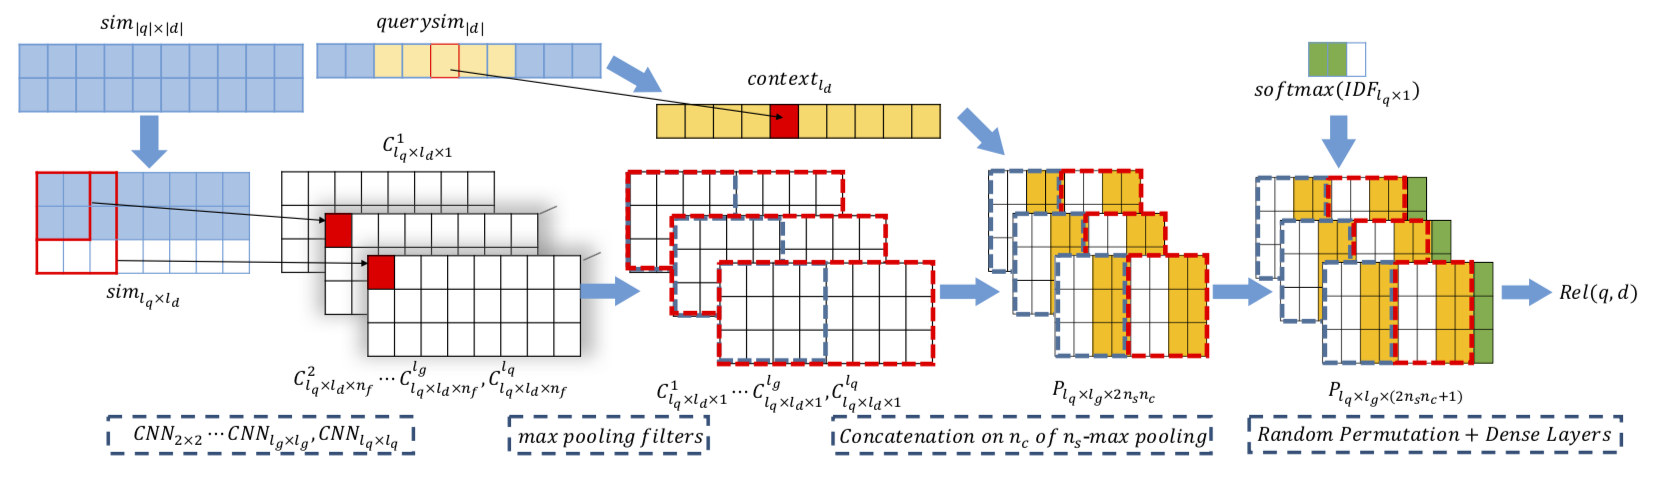
\includegraphics[width=\textwidth]{Figures/COPACRR.png}
%     \caption{CO-PACRR pipeline}
%     \label{fig:co_pacrr_pipeline}
% \end{figure*}

\section{Neural Pseudo-Relevance Feedback (NPRF-DRMM)}
\label{sec:nprf_drmm_reproducibility_desc}
In this work~\citep{li2018nprf}, they proposed a generic neural pseudo relevance feedback framework (NPRF) that helps the application of PRF with existing neural IR models (NIRM). For a given query and target document, NPRF produces a final relevance score by considering the interactions of the target document with the query as well as the top-$n$ feedback documents from the initial ranking (e.g. BM25, QL). The proposed framework directly incorporates existing neural IR models without the need to modify their architectures as shown in Figure~\ref{fig:nprf_drmm_pipeline}.

% \textbf{Initial ranking}. An initial ranking $rel_q(q, d)$ is applied to obtain the top-$n$ documents denoted as $D_q$ for $q$.

\textbf{Extracting document interactions}. Given the target document $d$ and each feedback document $d_q\in D_q$, $rel_d(d_q, d)$ is a NIRM that is used to compute the $n$ relevance scores. Since DRMM takes as input matching histograms (\textit{LCH}x\textit{IDF}) from the cosine similarity between pairs of term embeddings from $d$ and $d_q$ without considering term dependencies, so $d_q$ is summarized by keeping the top-$k$ terms based on \textit{tf-idf} scores to remove noisy or irrelevant terms.

\begin{figure*}
    \centering
    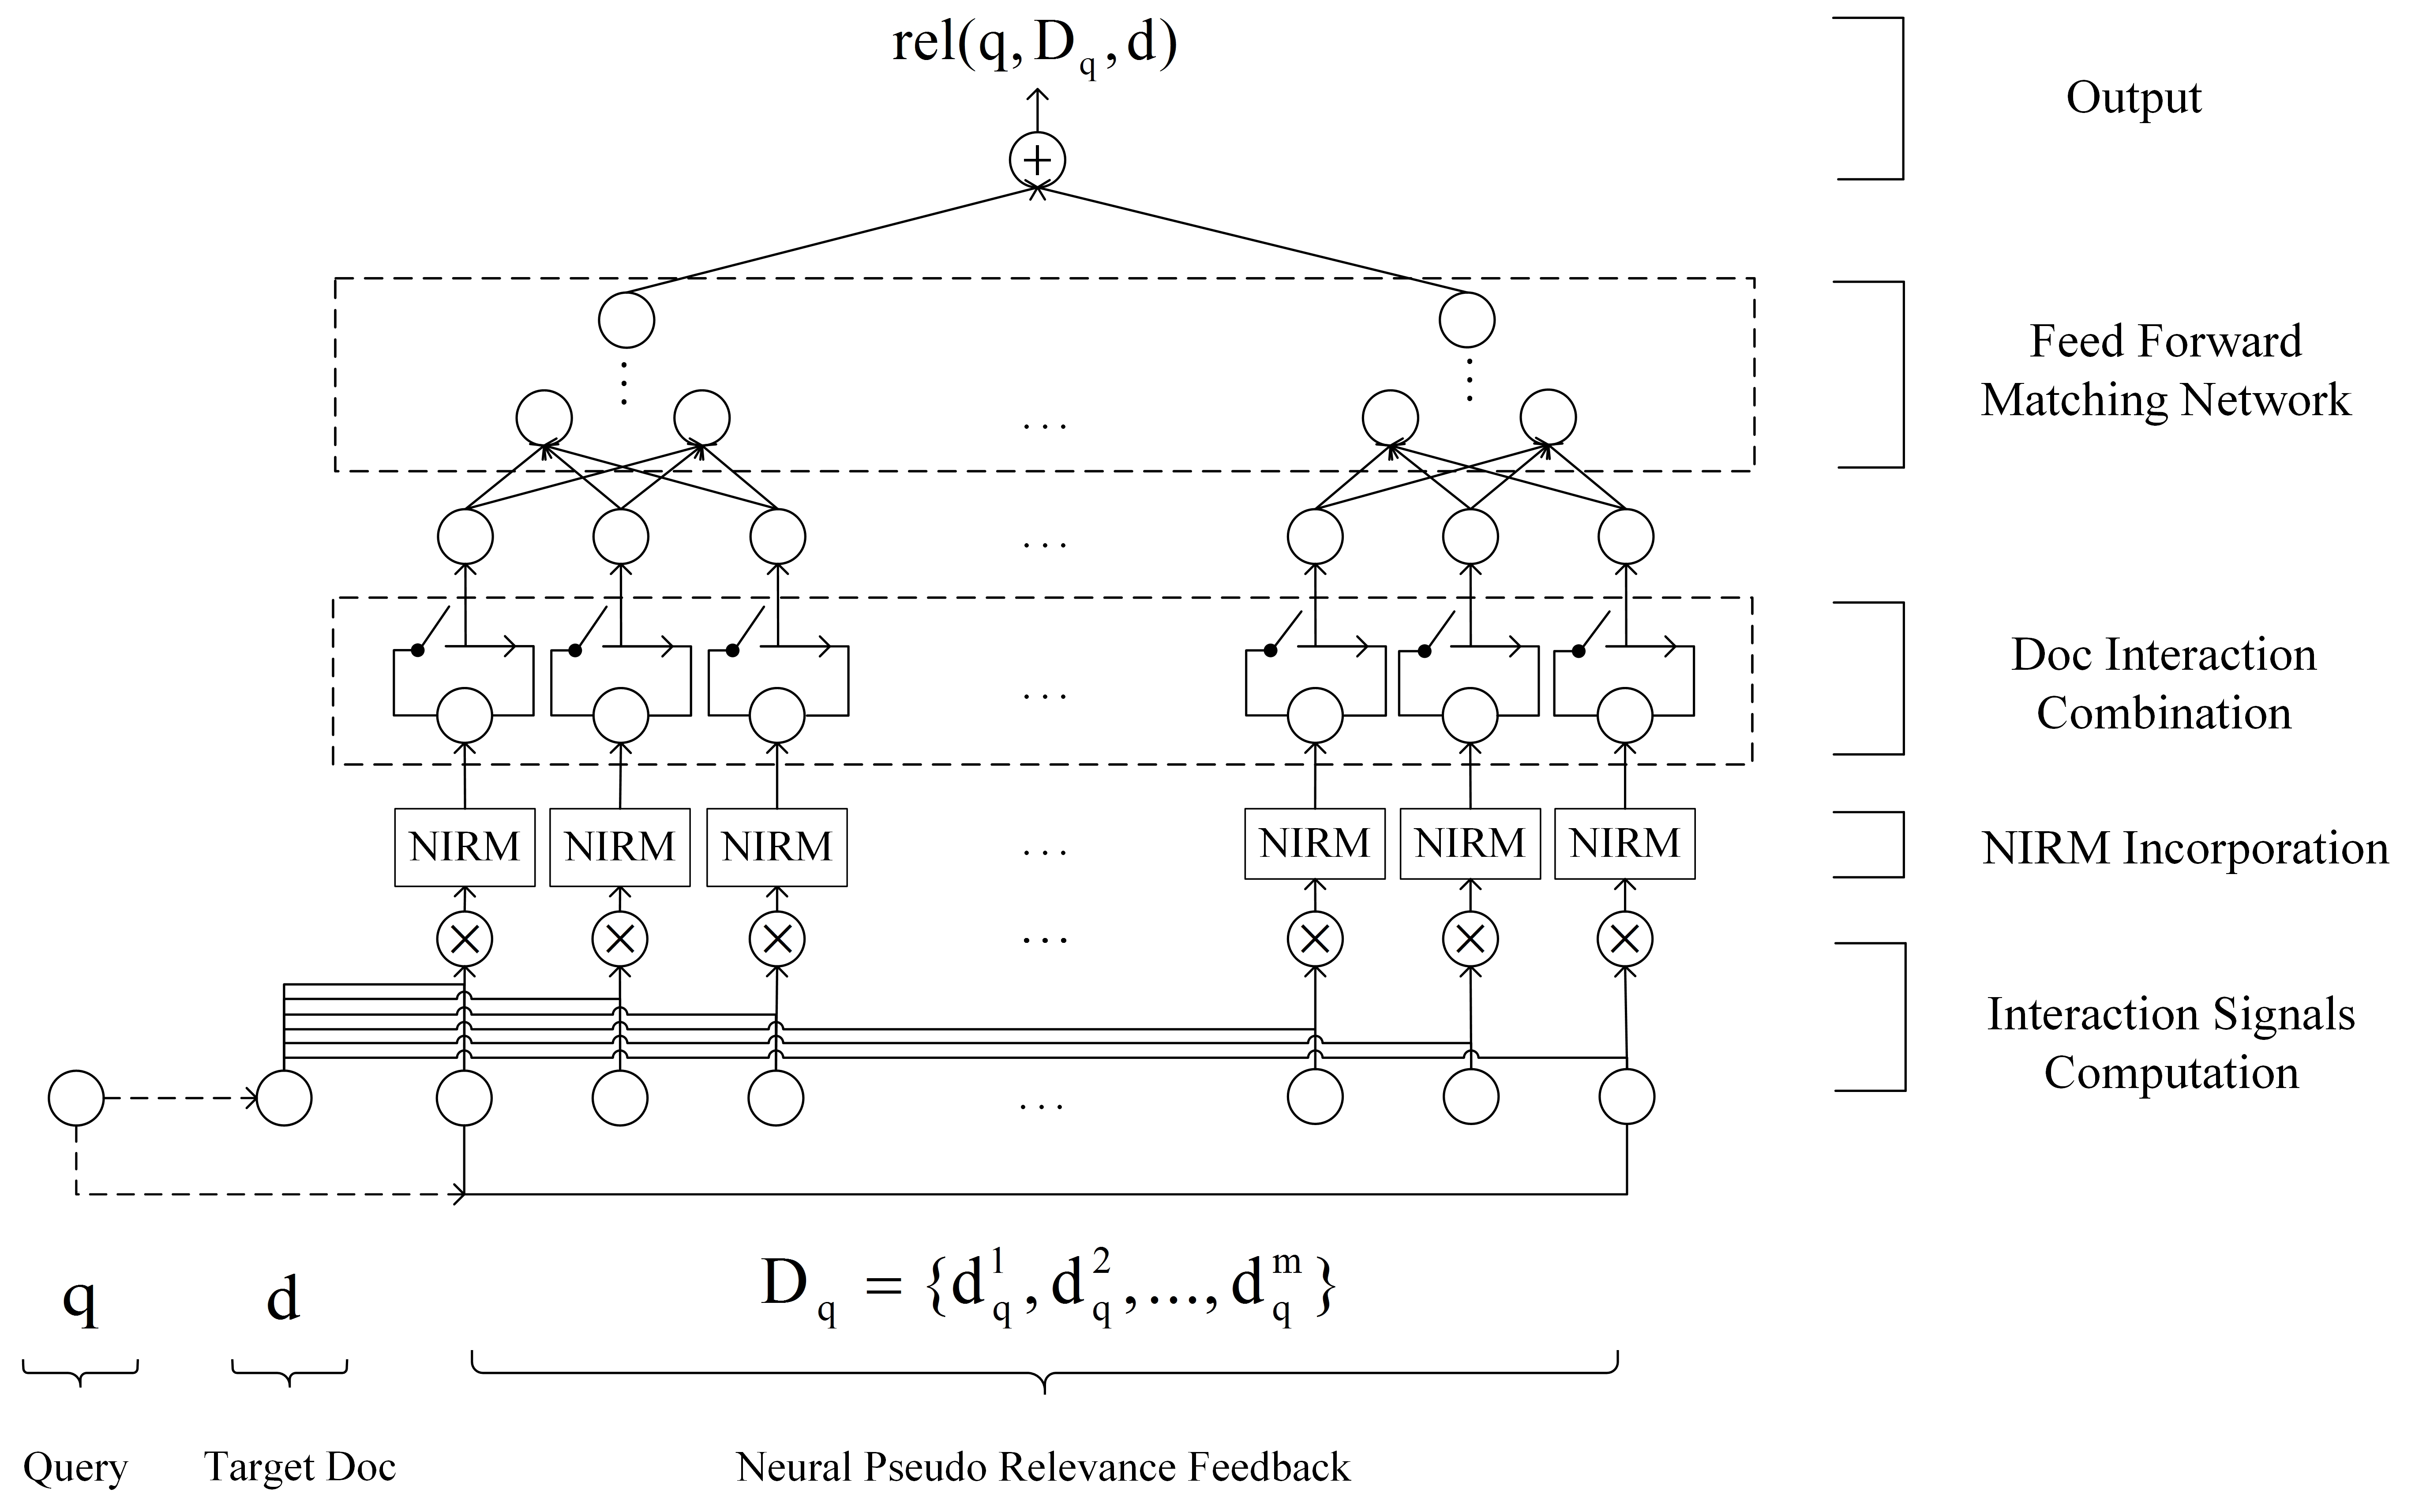
\includegraphics[width=14cm]{Figures/NPRF-arch.jpg}
    \caption{Neuro Pseudo Relevance Framework (NPRF) architecture~\citep{li2018nprf}}
    \label{fig:nprf_drmm_pipeline}
\end{figure*}

\textbf{Combining document interactions}. When combing the relevance scores for the feedback documents, the relevance of $d$ from the initial ranking $rel_q(q, d_q)$ is also important. Thus, weighted relevance document score $rel_d'(d_q, d)$ is computed using the equation~\ref{nprf_doc_rel} with min-max normalized $rel_q(q, d_q)$ score.
\begin{equation}\label{nprf_doc_rel}
    rel_{d}'(d_q, d) = rel_d(d_q, d)(0.5 + 0.5 * rel_q(q, d_q))
\end{equation}
The $rel_d'(d_q, d)$ of each $d_q \in D_q$ is combined into a single relevance score using two variants: (i) direct summation, and (ii) using feed forward network with \textit{tanh} activations.

\textbf{Training Objective}. A pairwise ranking loss such as hinge loss with a margin of 1.0 is used for training the model similar to the objective defined in eq.~\ref{eq:drrm_loss_objective}.

\subsection{Experimental Setup}
\label{sec:nprf_drmm_reproducibility_exp}

The indexing and retrieval experimental setup for the TREC Robust04 collection is the same as described in section~\ref{drmm_exp_setup}. The term embeddings used are the \texttt{word2vec} embeddings of 300 dimensions trained on the Robust04 collection using the setup described in section~\ref{drmm_exp_setup}. Akin to the evaluation setup for DRMM described in section~\ref{drmm_exp_setup}, the proposed NPRF\textsubscript{ds}-DRMM model is used to re-rank the top-2000 documents retrieved from BM25 and uses the same 5-fold cross validation setup to measure the model's retrieval performance.

\textbf{Model Implementation}. The model implemented in Keras is trained using the \texttt{Adam} optimizer with a batch size of 20 and an initial learning rate of $10^{-3}$ followed by step-decay learning rate schedule that drops the rate by a factor of 0.9 after every 25 iterations. Usually, the training converges within 30 epochs or maximum 250 iterations (on each iteration the model trains on 100 mini-batches). The variant that we implemented is NPRF\textsubscript{ds}-DRMM that is based on the direct summation of the weighted feedback document relevance scores as that was shown to have the best performance across all the variants~\citep{li2018nprf} on the TREC Robust04 collection. The top-10 documents from BM25 are used as the pseudo relevant feedback document input $D_q$ for the model, where each $d_q \in D_q$ is summarized by the top-20 terms based on \textit{tf-idf}. The network configuration for the DRMM component is using the DRMM\textsubscript{\textit{LCH}x\textit{IDF}} variant with the original configuration (\citep{Guo2016}) that includes a histogram input layer of 30 nodes, two hidden layers in MLP (5 and 1 node respectively), and one output node with term gating (\textit{IDF}-softmax values) for the feedback document relevance score. A different sampling strategy is used to generate the training pair instances that takes into consideration the data imbalance problem thus generating about the same number of pairs across all the queries even if some queries have more positive samples than others\footnote{\url{https://github.com/ucasir/NPRF/blob/master/utils/pair_generator.py\#L100}}.

\subsection{Results and Discussion}
\begin{table}[]
    \centering
    \begin{tabular}{lccc}
    \toprule
        Model Name & MAP & nDCG@20 & P@20 \\
        \midrule
        BM25 & 0.2405 & 0.4038 & 0.347 \\
        %PACRR & 0.260 & 0.442 & 0.372\\
        NPRF\textsubscript{ds}-DRMM & 0.2869 & 0.4585 & 0.4006 \\
        NPRF\textsubscript{ds}-DRMM \textit{paper} & 0.2904 & 0.4502 & 0.4064 \\
    \bottomrule
    \end{tabular}
    \caption{NPRF-DRMM model retrieval performance on the Robust04 collection}
    \label{tab:nprf_drmm_eval}
\end{table}
From Table~\ref{tab:nprf_drmm_eval}, we see that NPRF\textsubscript{ds}-DRMM shows significant improvements over the BM25 baseline across all evaluation metrics. We also see that the model trained using the architecture configuration mentioned above, gives a retrieval performance that is quite close to the model trained in the paper across all the metrics. This is because we used the same partitions of the topics shared by the authors as part of the code\footnote{\url{https://github.com/ucasir/NPRF/blob/master/model/nprf_drmm_config.py}}. The small differences in the metrics is because the preprocessing that we used is different from that mentioned in the paper where they used a porter stemmer instead of krovetz stemmer and also the word embeddings are trained differently by using the pool of top-2000 documents returned from BM25 for each individual queries as suggested by~\cite{diaz16} instead of the entire Robust04 collection as we used in section~\ref{drmm_exp_setup}.

%-----------------------------------------------------
%	SECTION 5
%-----------------------------------------------------
\section{Deep Structured Semantic Models (DSSM)}
The Deep Structured Semantic Model (DSSM)~\citep{dssm13} is based on Siamese networks used for short text matching. The model is trained on pairs of query and documents titles, both texts represented as a bags-of-character-trigraphs. This architecture consists of two deep models--for the query as well as the document--with fully-connected layers and cosine distance as the similarity function. They train the model on clickthrough data where each sample consists of a query \textit{q}, positive documents $d^{+}$ (document clicked by user on SERP page) and a set of negative documents $D^{-}$ randomly sampled uniformly from the collection. The model is trained by minimizing the cross-entropy loss after taking a softmax over the model outputs for all the candidate documents,
\begin{equation}
\begin{split}
	\mathcal{L}_{DSSM}(q,d^+,D^-) = \
    {\log (\frac{e^{\gamma \cdot \cos (\vec{q},\vec{d^+})}}{\sum_{d \in D}e^{\gamma \cdot \cos (\vec{q},\vec{d})}})} \\
    where, D = {d^+} \cup D^-
\end{split}    
\end{equation}
\begin{figure}
    \centering
    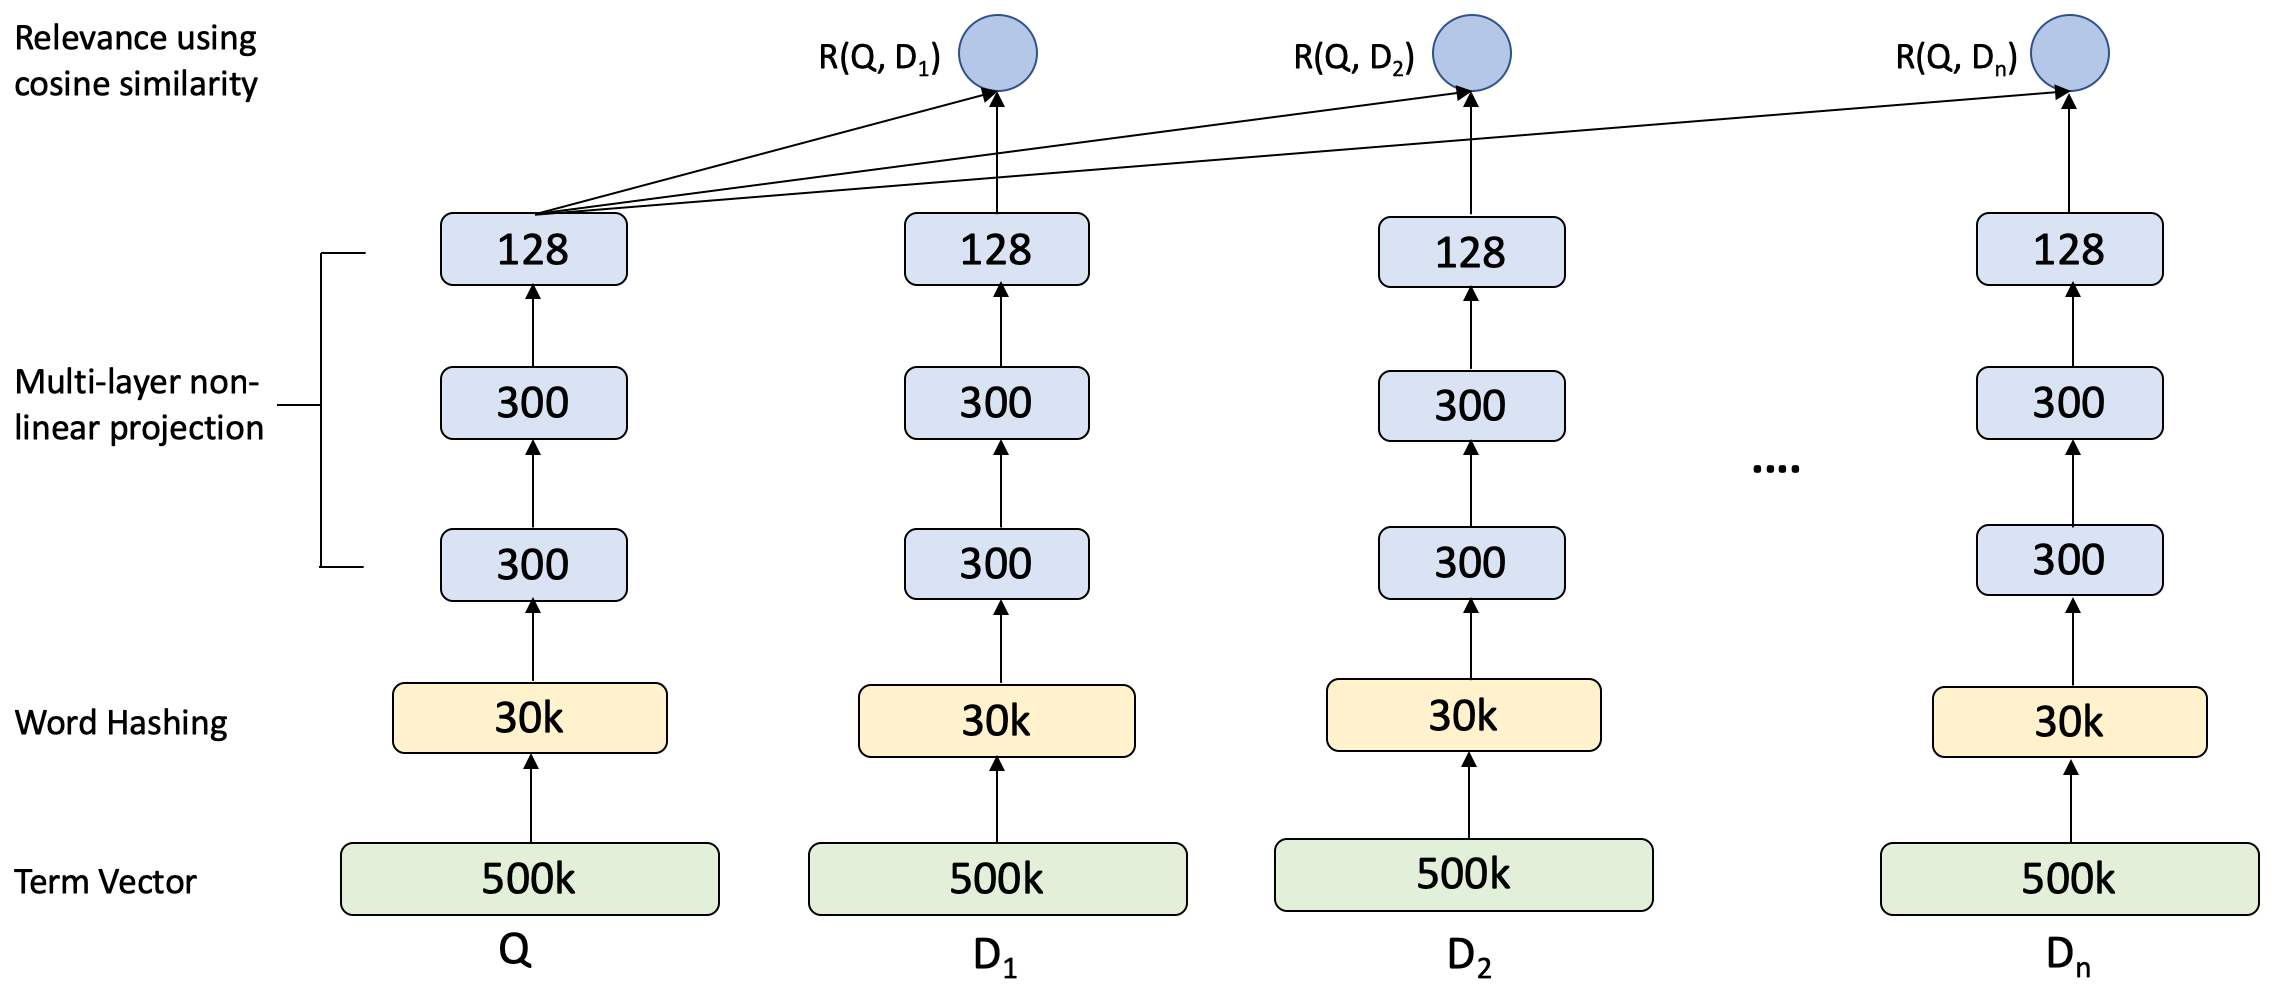
\includegraphics[width=12cm]{Figures/dssm_ppt.png}
    \caption{Deep Structured Semantic Model (DSSM) architecture
    %The first hidden layer with 30k units, accomplishes word hashing. The word-hashed features are then projected through multiple layers of non-linear projections. The final layer output produces the low-dimensional dense vector in the semantic space.
    }
    \label{fig:dssm_architecture}
\end{figure}

\subsection{Experimental Setup}
The indexing and retrieval experimental setup for the TREC Robust04 collection is the same as described in Section~\ref{drmm_exp_setup}. Since DSSM needs large scale training data (large click-through dataset), due to its huge parameter size, we try to train the model using two strategies: pretraining the triletter embeddings using the Robust04 collection instead of training it during model training, and using weak supervision to train the model with AOL query logs as suggested by~\cite{Dehghani_sigir17}. The models implemented in Keras are trained using the \texttt{Adam} optimizer with varying batch sizes and learning rates. The parameters of the DNN is shown in Figure~\ref{fig:dssm_architecture}, the only difference is that the number of nodes in the word hashing layer depends on the triletters obtained from the Robust04 collection.

\subsubsection{Pretraining Triletter Embeddings}

The input for the DSSM model is the bag-of-character triletter vector which is of much lower dimensionality ($\sim$15k) than term vectors which are usually the size of the vocabulary ($\sim$500k), thus enabling us to effectively train a deep neural network (DNN). Due to the limited number of queries and smaller size of the training dataset from Robust04 collection in comparison to the Bing Web collection that is used in the paper, we first train the triletter embeddings from the collection so that the limited training data can then be used to effectively learn dense representations for both queries and documents.

The 300 dimensional triletter embeddings are trained using the skip-gram model with negative sampling (SGNS)~\citep{Mikolov2013}. The corpus is preprocessed removing HTML tags, but no stemming and stopword removal is applied. Each word (e.g. \textit{good}) in the collection is first represented with starting and ending marks (e.g. \textit{\#good\#}) after which they are split into triletter \textit{n-grams} (e.g. \textit{\#go, goo, ood, od\#}). The corpus then comprises of documents represented using the triletters instead of words which are then used to train the embeddings. The parameters used are context window size (5), negative samples (10), minimum triletter frequency (5) and subsampling of frequent words with a threshold of $10^{-4}$ using \texttt{word2vec}\footnote{\url{https://radimrehurek.com/gensim/models/word2vec.html}} (\texttt{sg=1} and \texttt{hs=0}). The model is trained for 20 epochs over the corpus. The parameters for the model were chosen based on~\cite{ngram_embeddings17}, where they describe how to compute word embeddings by training \textit{n-gram} embeddings and then representing each word by the sum of these representations.

\subsubsection{Weak supervision with AOL query logs}

\textbf{Training query set}. We prepare the training query set using the setup described in~\cite{Dehghani_sigir17}, which comprises of unique queries that appear in the AOL query logs. We filter out navigational queries containing URL substrings (``http'',``www.'', ``.com'', ``.net'',``.org'', ``.edu''). All non-alphanumeric characters from the queries were removed. All queries that are present in the evaluation Robust04 queries are removed from the training set. Finally, only those queries that have at-least 10 documents retrieved by BM25 from Robust04 are kept, thus giving us a set of 6.15 million queries are after preprocessing. We also created smaller subsets of queries (1k, 10k) to see if we can effectively train a small model and 1M as that should already give us sufficient data to train the model.

\textbf{Training data}. In~\cite{Dehghani_sigir17}, they retrieve the top-1000 documents using BM25 for each query in the training query set and generate $|Q|$x$1000^2$ ($\sim$6E13) pairwise training pairs. Due to limited computational resources and time, we used different sampling strategies to generate the pairs:
\begin{itemize}
    \item For each positive document that we consider from the top-10, we sample 4 negative documents from the rest of the top-1000 documents.
    \item For each positive document from the top-10, we sample 3 negative documents randomly from the rest of the collection and 1 negative document from the rest of the top-1000 based on probability distribution over the BM25 scores.
    \item For each positive document from top-10, we sample 4 negative documents from the rest of the collection.
    \item For a positive document from top-1, we randomly sample 4 negative documents from the rest of the collection.
\end{itemize}

\textbf{Document text}. In the DSSM paper, they train the model on query-document title pairs where title is extracted from the title field from the index. Thus, we also tried training the model on different document text versions since the Robust04 collection doesn't have a specific title field in many of the documents ($\sim$65\%)-- full-text of document, the first 3 sentences of the document as the title, the first 2 sentences as the title and the first 3 sentences plus the snippet as title for the positive documents.

\subsection{Results and Discussion}

Using the various strategies described above to train the DSSM model, we couldn't effectively train a model that performs better than BM25 baseline\footnote{\url{https://www.comet.ml/neural-ir/dssm-weak-supervision}}. The poor effectiveness of the DSSM model (\textit{representation-focused}) is also highlighted in previous studies~\citep{Guo2016, matchpyramid16}. One possible reason for the poor effectiveness is that it is difficult to learn a good global representation of the documents in the Robust04 collection to match with the representation learnt for a related query.

However, these results are inconsistent with that of~\cite{Dehghani_sigir17} where they show a model based on representation learning and weakly supervised with BM25, gives a performance better than BM25. Our results with weak supervision reflects the same performance as in this study~\citep{Nie_ictir18}, where they hypothesize that the difference in performance could be due to the huge difference in computation resources where they train a very large number of training pairs ($\sim$6E13) for a large number of epochs. One other reason could be that the size of the dense input representation has a much smaller dimensionality (300-dimension normalized weighted element-wise summation of the term embeddings) whereas for DSSM it is about 15k.

% \clearpage
\section{Performance Comparison of Trained Models}
\label{sec:compare_perform_trained models}
In this section, we briefly compare the retrieval performance of the implemented neural retrieval models as seen in Table~\ref{tab:comparison_all_model_eval}. We can see that all of the implemented neural retrieval models perform better than the traditional BM25 baseline as highlighted in previous work, except for MatchPyramid which is similar to the conclusion they get in the original paper~\citep{matchpyramid16}. 

We can clearly observe that \textit{position-aware} neural IR models, like, PACRR and PACRR-DRMM that takes into consideration the context of the query terms perform better than DRMM which computes the interactions between the query and document terms ignoring the context. Also, we see that the NPRF model (NPRF\textsubscript{ds}-DRMM) which incorporates pseudo relevance feedback into the existing DRMM model, improves on the DRMM retrieval performance across all evaluation metrics. We also provide a comparison of the hyper-parameters between the implemented neural retrieval models in Table~\ref{tab:hyperparam_all_models}.

\begin{table}[]
    \centering
    \begin{tabular}{llcccc}
        \toprule
         Models & Model Name & MAP & nDCG@20 & P@20\\
         \midrule
         Traditional IR & BM25 & 0.2405 & 0.4038 & 0.347\\ 
         \cmidrule(lr){1-5}
         
         \multirow{1}{*}{DRMM} & DRMM\textsubscript{\textit{LCH}x\textit{IDF}} & 0.257 & 0.4103 & 0.352 \\
        %  & DRMM\textsubscript{\textit{LCH}x\textit{IDF}} \textit{paper} & 0.268 & 0.423 & 0.381\\
         \cmidrule(lr){1-5}
         
         \multirow{2}{*}{MatchPyramid} & MP-Ind & 0.1823 & 0.3353 & 0.286\\
        %  & MP-Ind \textit{paper} & 0.169 & 0.319 & 0.281 \\
         & MP-Cos & 0.1898 & 0.3328 & 0.276\\
        %  & MP-Cos \textit{paper} & 0.189 & 0.330 & 0.290\\
         \cmidrule(lr){1-5}
         
         \multirow{2}{*}{PACRR-DRMM} & PACRR & 0.260 & 0.442 & 0.372\\
         & PACRR-DRMM & 0.263 & 0.445 & 0.374 \\
        %  & PACRR-DRMM \textit{paper} & 0.259 & 0.444 & 0.373 \\
         \cmidrule(lr){1-5}
         
         \multirow{1}{*}{NPRF} & NPRF\textsubscript{ds}-DRMM & 0.2869 & 0.4585 & 0.4006 \\
        %  & NPRF\textsubscript{ds}-DRMM \textit{paper} & 0.2904 & 0.4502 & 0.4064 \\
         \bottomrule
    \end{tabular}
    \caption{Comparison of retrieval performance across different retrieval models on Robust04 collection}
    \label{tab:comparison_all_model_eval}
\end{table}

\begin{table}[h]
    \footnotesize
    \centering
    \begin{tabular}{lllll}
        \toprule
         Hyper-parameters &  DRMM & MatchPyramid & PACRR-DRMM & NPRF-DRMM\\
         \midrule
         Initial learning rate (\textit{lr}) & $10^{-3}$ & $10^{-4}$ & $10^{-3}$ & $10^{-3}$\\
         
         Step-decay (\textit{lr}) & \checkmark & \checkmark & \xmark & \checkmark\\
         
         Drop factor (\textit{lr}) & 0.9 (10 iter.) & 0.9 (10 iter.) & --- & 0.9 (25 iter.)\\
         
         Mini-batch size & 20 & 32 & 32 & 20\\
         
         Optimizer & Adam & Adam & Adam & Adam\\
         
         Training iterations & 100 & 200 & 50 & 250\\
         
         Nr. mini-batches per iter. & 1000 & 1000 & --- & 100\\
         
        %  Nr. training pairs sampled & 2M & 6.4M & all & 0.5M\\
         \bottomrule
    \end{tabular}
    \caption{Comparison of hyper-parameter values across the different retrieval models}
    \label{tab:hyperparam_all_models}
\end{table}

\section{Deployment of Trained Models}\label{sec:deploy_nrm}

\begin{figure}[h]
    \centering
    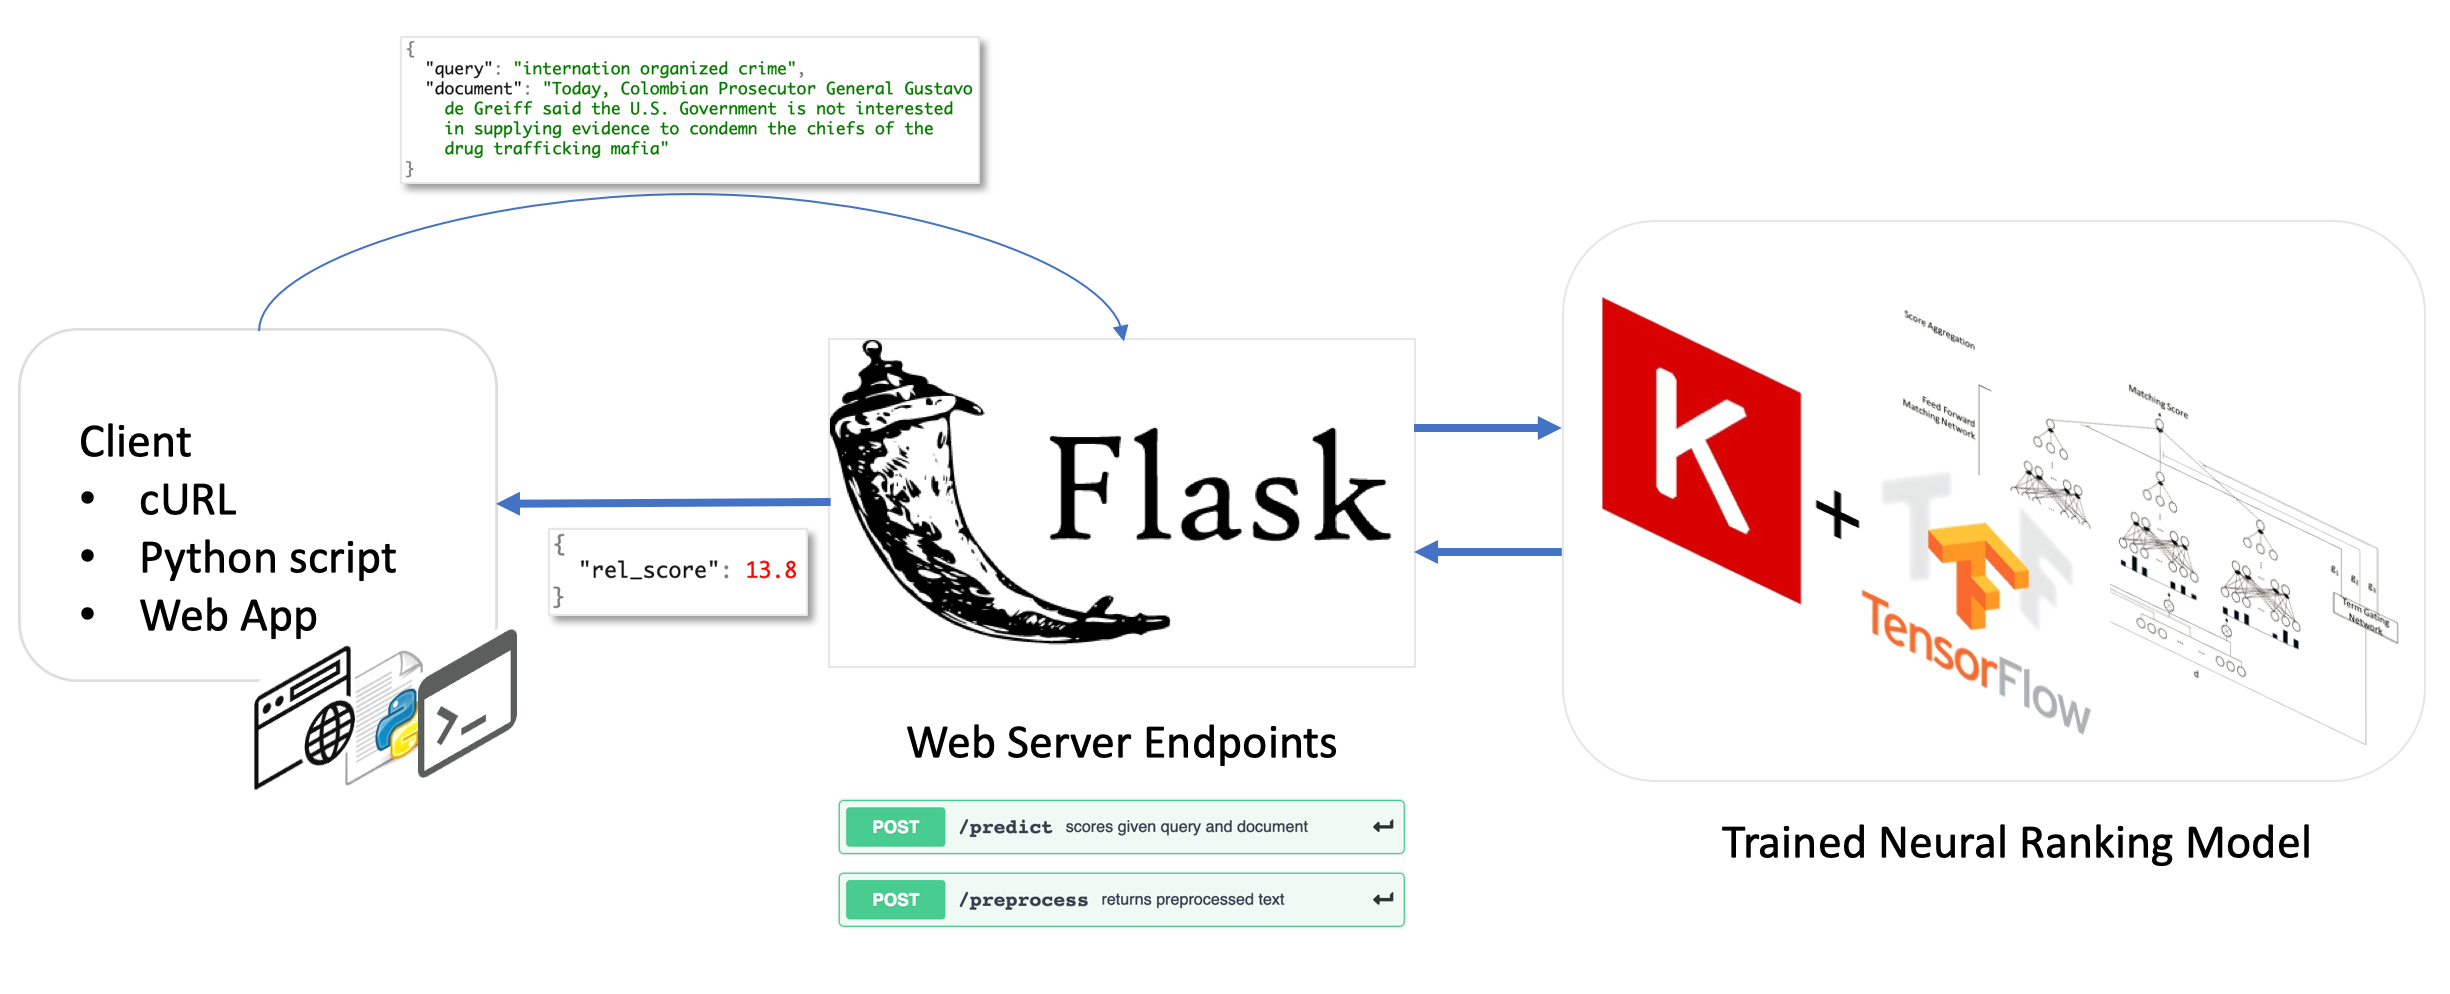
\includegraphics[width=\textwidth]{Figures/trained_model_deploy2.png}
    \caption{Deployment of NRMs workflow}
    \label{fig:nrm_deployment}
\end{figure}
% \clearpage
We have deployed some of the trained models (DRMM, MP-COS, PACRR-DRMM, NPRF\textsubscript{ds}-DRMM) using the Flask\footnote{\url{http://flask.pocoo.org/}} web framework. The Flask server first loads the pretrained Keras model that shows the best performance on MAP for Robust04 and exposes two REST API endpoints--for scoring a given query-document pair and for preprocessing the given text into the input format required by the pretrained model. The work flow of how the models are deployed is displayed in Figure.~\ref{fig:nrm_deployment}.

The endpoint for scoring can be used by any system that has a \textit{telescoping} setup that has to re-rank the initial set of retrieved documents (e.g. BM25 or QL) using one of the trained models. The second endpoint for preprocessing the given text is useful for interpretable visualizations such as heatmaps that highlights words in the document that are relevant/irrelevant to the query.
 
\chapter{Interpretability in IR} % Main chapter title

\label{Chapter5} % Change X to a consecutive number; for referencing this chapter elsewhere, use \ref{ChapterX}

\lhead{Chapter 5. \emph{Interpretability in IR}} % Change X to a consecutive number; this is for the header on each page - perhaps a shortened title

In this chapter, we will initially describe how the interpretability approaches detailed in chapter~\ref{Chapter3}--LIME (section~\ref{sec:lime_approach}) and DeepSHAP (section~\ref{sec:deepshap_approach}) are applied for \textit{ad-hoc} text retrieval and ranking in the context of complex neural ranking models. 

In this work, we are interested in how DeepSHAP can be adapted to explain the output of neural retrieval models (NRM). In particular, what is a good ``\textit{reference}'' input in the context of IR? In computer vision, a plain black image is a good reference input to understand the decisions of a image classifier. So we developed various reference input document construction methods as described in the section~\ref{sec:deepshap_ir} for 3 different neural rankers (DRMM, MatchPyramid, PACRR-DRMM). We would also like to investigate if DeepSHAP's explanations are highly sensitive or robust to the different reference input distributions that were constructed. Also, do these reference input distributions perform differently depending on the neural ranking model. Additionally, we compare the explanations produced by DeepSHAP to that of LIME (model-agnostic) detailed in section~\ref{sec:lime_ir}. We ponder on the question, if both these approaches produce different or similar explanations, as they both give \textit{local} explanations. 

In order to understand the various questions raised above, we describe the experimental setup in section~\ref{sec:lime_shap_exp_setup}. The results of the various experiments are discussed in detail in section~\ref{sec:lime_shap_results}.

%-----------------------------------------------------
%	SECTION 1
%-----------------------------------------------------
\section{LIME for IR}\label{sec:lime_ir}

\begin{figure}[]
  \centering
  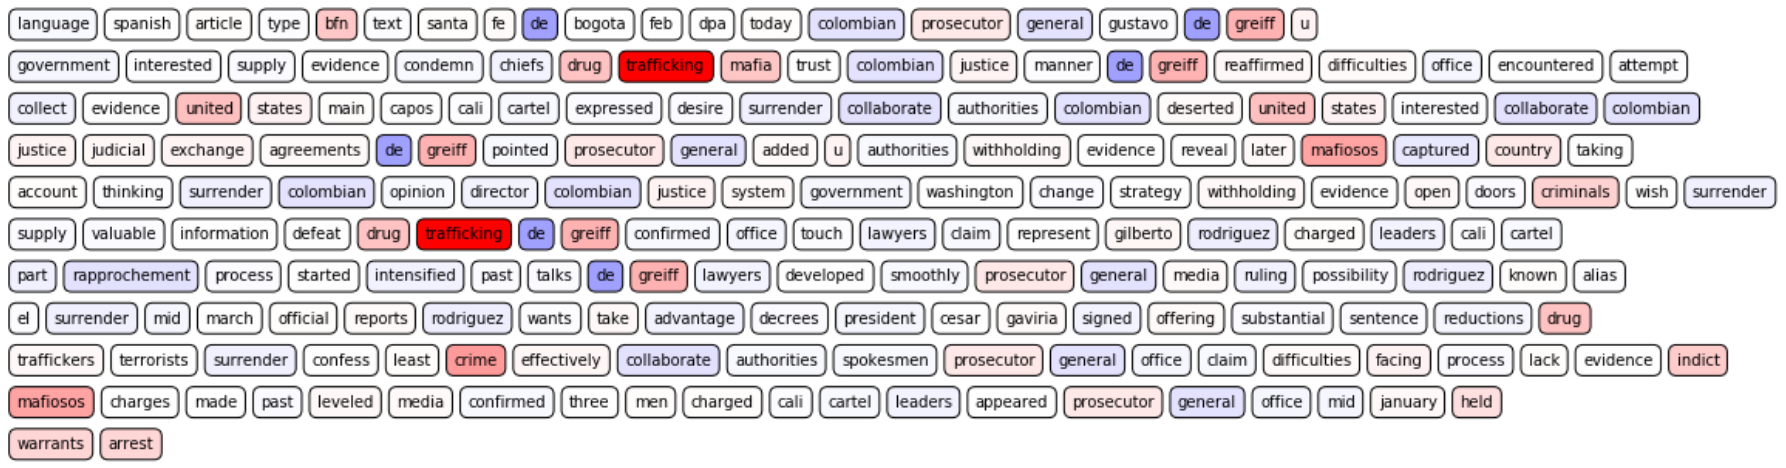
\includegraphics[width=\textwidth]{Figures/q301_FBIS3-10082_lime_drmm.png}
  \caption[Heatmap visualization of document using LIME relevance weights for DRMM.]{Heatmap visualization over the words in the doc `\textsf{FBIS3-10082}' for the query `\textsf{international organized crime}' using the output of LIME for the DRMM ranking model. \textit{Words highlighted in `red' indicate `relevance' and those in `blue' for the `irrelevant' class.}}
  \label{fig:drmm_lime_heatmap}
\end{figure}

The LIME~\citep{Ribeiro16} approach is designed mainly to explain the output of classifiers, whereas we would like to understand \textit{why} a particular document returned from a neural retrieval model is relevant to a query. Recently, there has been work~\citep{Singh19} which adapted LIME to show how ranking can be cast as a classification problem where the neural retrieval model predicts a class distribution (\textit{relevant} or \textit{irrelevant}) for a given query-document pair. We discuss their {\it score-based} approach that we implemented here, consider a query {\it q} and the list of {\it top-k} documents $D^{k}_{q}$ returned from the neural retrieval model $\mathcal{R}$ (point-wise ranker) obtained by scoring each document from a set of candidate documents retrieved from the index (BM25) and sorting. To explain a document $d$ from $D^{k}_{q}$, LIME trains an explanation model $\mathcal{M}_{d}$ on the perturbed documents $d'$. To model it into a classification problem they consider a random variable $\mathcal{X}$ to indicate the possible classes - \textit{relevant} and \textit{irrelevant}. Below is the formula used to compute $P(\mathcal{X} = relevant|q,d',\mathcal{R})$ using the {\it score-based} approach,
\begin{equation}
    1 - \frac{\mathcal{R}(q,d_{1}) - \mathcal{R}(q,d')}{\mathcal{R}(q,d_{1})}
\end{equation}
where $d_{1} \in D^{k}_{q}$ is the top-ranked document in the list, if $\mathcal{R}(q,d') \geq \mathcal{R}(q,d_{1})$ then $P(\mathcal{X}=relevant) = 1$. Note that $P(\mathcal{X} = irrelevant|q,d',\mathcal{R}) = 1 - P(\mathcal{X} = relevant|q,d',\mathcal{R})$.

\textbf{Explanation Model} In this approach the interpretable feature space is the set of words and since the explanation model $\mathcal{M}_{d}$ is a linear ridge regression model, the sign and magnitude of the coefficients of $\mathcal{M}_{d}$ indicate which words in $d$ are strong indicators of relevance and could be used as visual explanations such as heatmaps over the input words as shown in Figure~\ref{fig:drmm_lime_heatmap}.


\section{DeepSHAP for IR}\label{sec:deepshap_ir}

In the context of IR, DeepSHAP can be used to explain \textit{why} a document is relevant to query (according to a given neural retrieval model) by computing the shapley values for words in the document. The words with high shapley values indicate that they are important towards this prediction of relevance. However, to accurately compute the shapley values using DeepSHAP--a reference input is needed. What makes a good \textit{background} image in the context of IR? 

Unlike classification tasks, in ranking we have at least 2 inputs which are in most cases the query and document tokens. In this work, we fix the reference input for the query to be same as that of the query-document instance to be explained and experiment with various reference inputs for the document. The intuition behind doing so is to gain an average reference output in the locality of the query. 

The various document reference inputs that we considered in our experiments are:
\begin{description}
    \item[OOV] The reference document consists of `OOV' tokens. For, DRMM and MatchPyramid models the embedding vector for `OOV' comprises of all-zeros which is similar to the background image used for MNIST. But for PACRR-DRMM the `OOV' embedding vector is the average of all the embedding vectors in the vocabulary. 
    \item[IDF {\it lowest}] The reference document is constructed by sampling words with low IDF scores. These words are generally stop-words or words that are similar to stop-words so they should, in general, be irrelevant to the query. 
    \item[QL {\it lowest}] The reference document comprises of sampled words with low {\it query-likelihood} scores that are derived from a language model of the {\it top-1000} documents. As this would have words that are irrelevant to the query, SHAP should be able to pick more relevant terms from the document to be explained.
    \item[COLLECTION {\it rand doc}] The reference document is randomly sampled from the rest of the collection minus the {\it top-1000} documents retrieved for the query.
    \item[TOPK LIST {\it rand doc from bottom}] The reference document is randomly sampled from the bottom of the {\it top-1000} documents retrieved.
\end{description}

These variants were designed based on the intuition that the reference input document would comprise of words that are irrelevant to the query and thus DeepSHAP should be able to pick the most important terms from the input document that explain relevance to the query.

\section{Experimental Setup}
\label{sec:lime_shap_exp_setup}
In our experiments, we aim to answer the following research questions:

\begin{itemize}
    \item \textbf{RQ1} Are DeepSHAP explanations sensitive to the type of reference input in the case of NRMs?
    \item \textbf{RQ2} Can we determine which reference input produces the most accurate local explanation?
    \item \textbf{RQ3} Does modeling the reference distribution for query input also affect the DeepSHAP explanations?
\end{itemize}

To this end, we describe the experimental setup we used to address these questions. The 3 neural ranking models that we considered are--DRMM, MatchPyramid (MP-COS), and PACRR-DRMM. All the models were trained using the setup as described in chapter~\ref{Chapter4}. Once trained all the models were deployed using the Flask web framework as detailed in section~\ref{sec:deploy_nrm}.

To conduct the experiments, we used the Robust04 test collection from TREC. We used Lucene to index and retrieve documents. We chose to study explanations for the distinguished set of hard topics\footnote{\url{https://trec.nist.gov/data/robust/04.guidelines.html}} (50) from the TREC Robust Track 2004 (model retrieval effectiveness highlighted in Tab~\ref{tab:robust04_difficult_rank_measures}). We generate the explanations from LIME and SHAP for the top-3 documents retrieved for each query and use only these for our quantitative experiments.

\begin{table}[h]
\centering
\begin{tabular}{lcccccc} 
 \toprule
 & MAP & MRR & P@10 & P@20 & NDCG@10 & NDCG@20\\
 \midrule
 BM25 & 0.0890 & 0.4786 & 0.2280 & 0.2030 & 0.2462 & 0.2289\\
 DRMM & 0.1202 & 0.5444 & 0.2900 & 0.2430 & 0.3103 & 0.2781\\
 MatchPyramid & 0.0855 & 0.4466 & 0.2420 & 0.2140 & 0.2512 & 0.2340\\
 PACRR-DRMM & 0.1036 & 0.4704 & 0.2720 & 0.2310 & 0.2780 & 0.2545\\
 \bottomrule
\end{tabular}
\caption{Overview of models retrieval effectiveness for the ROBUST04 hard queries}
\label{tab:robust04_difficult_rank_measures}
\end{table}

\textbf{Evaluating explanations} Since no ground truth explanations are available for a neural model, we use LIME based explanations as a proxy. Although LIME is model agnostic, we found that it can accurately model relevance for a given query document pair using a simple linear model over words. Table~\ref{tab:lime_model_performances} shows this observation, where the number of perturbed samples for every query-document pair is divided into train (90\%) and test (10\%) splits. To produce the explanations from LIME we used the implementation found in \footnote{\url{https://github.com/marcotcr/lime}} along with the score-based modification described in section~\ref{sec:lime_ir}. The primary parameters for training a LIME explanation model are the number of perturbed samples to be considered and the number of words for the explanation. The number of perturbed samples is set to 5000 and the number of words is varied based on the experiment. We used the DeepSHAP implementation provided here~\footnote{\url{https://github.com/slundberg/shap}}. Note that we ignore the polarity of the explanation terms provided by both methods in our comparison since the semantics behind the polarities in LIME and DeepSHAP are different. We are more interested in the terms chosen as the explanations in both cases.

For the SHAP explanations we used the methods as described in Section \ref{sec:deepshap_ir}. Since the model inputs for MatchPyramid and PACRR-DRMM directly accept document tokens it is a one-to-one mapping from the tokens to the corresponding SHAP value. But for DRMM, the model inputs are query-document histograms and thus we obtain SHAP values for these histogram buckets. So in order to map these SHAP values back to the document tokens we store a mapping from the tokens to their respective histogram buckets.

\begin{table}
\centering
\begin{tabular}{lcccc} 
 \toprule
 &\multicolumn{4}{c}{Linear Regression (Ridge)}\\
 NRM & TRAIN MSE & TEST MSE & TRAIN ACC & TEST ACC\\
 \midrule
 DRMM & 0.00631 & 0.00633 & 0.92662 & 0.92654\\
 MatchPyramid & 0.01827 & 0.01839 & 0.90367 & 0.90387\\
 PACRR-DRMM & 0.00165 & 0.00160 & 0.98857 & 0.98980\\
\bottomrule
\end{tabular}
\footnotesize
\caption[Evaluation of LIME's linear model performance metrics across various NRMs.]{Comparison of mean squared error (MSE) and accuracy (ACC) of LIME's linear model across various NRMs. Low MSE and high accuracy shows that it is able to fit and generalize in the query-document locality.}
\label{tab:lime_model_performances}
\end{table}


\section{Results and Discussion}
\label{sec:lime_shap_results}

\subsection{RQ1. Effect of reference input document} \label{sec:interpretability_rq1}

The top row in Figure~\ref{fig:shap_confusion_matrices} illustrates the overlap in terms of jaccard similarity between the explanation terms produced when varying the reference input. Immediately we observe that the overlap between explanations produced is low; below 50\% in most cases and consistently across all NRMs. Each reference input method has its own distinct semantics and this is reflected by the low overlap scores. This is also shown by the high Jensen-Shannon divergence scores (2nd row in Fig.~\ref{fig:shap_confusion_matrices}) between the probability distributions of the term coefficients returned by each reference input method. We also find that there is no consistent trend across NRMs. For MatchPyramid, \textsf{OOV} and \textsf{QL} have highest overlap whereas for PACRR-DRMM its \textsf{OOV} and \textsf{COL} that have highest overlap even though both models have the same input representation and parts of the model architecture are similar (convolutional and max-pooling layers). Table~\ref{tab:drmm_qualitative_example} shows explanations for DRMM across all variants. Once again we see how the explanations can differ significantly if we are not careful in selecting the reference input. For IR, finding the background image seems to be a much harder question. 

Our results show how explanations are highly sensitive to the reference input for NRMs chosen in our experiments. This is also indication that a single reference input method may not be the best for every NRM. 

\begin{figure}
  \centering
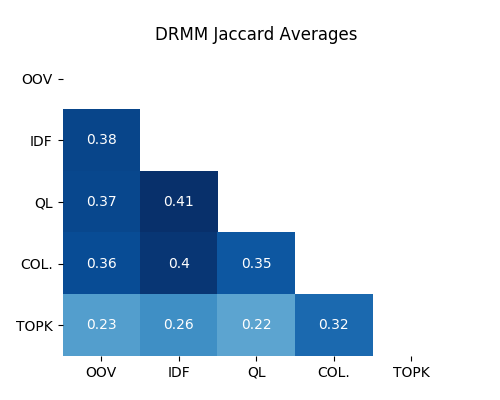
\includegraphics[width=.33\linewidth]{Figures/drmm_jaccard.png}\hfill
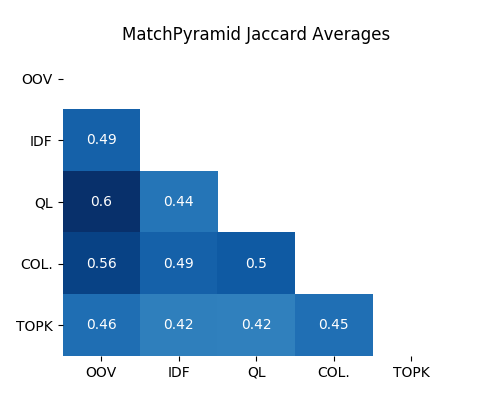
\includegraphics[width=.33\linewidth]{Figures/mp_cos_jaccard.png}\hfill
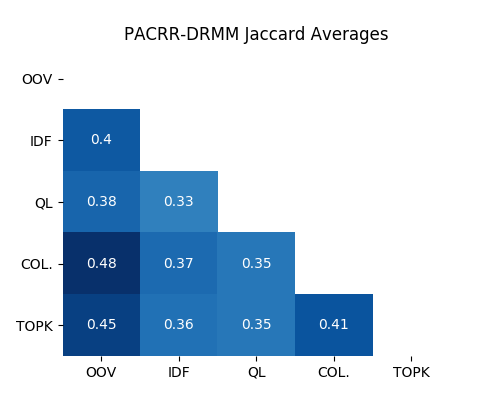
\includegraphics[width=.33\linewidth]{Figures/pacrr_drmm_jaccard.png}
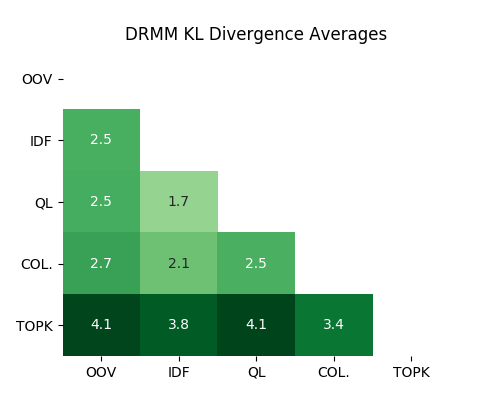
\includegraphics[width=.33\linewidth]{Figures/drmm_kl_div.png}\hfill
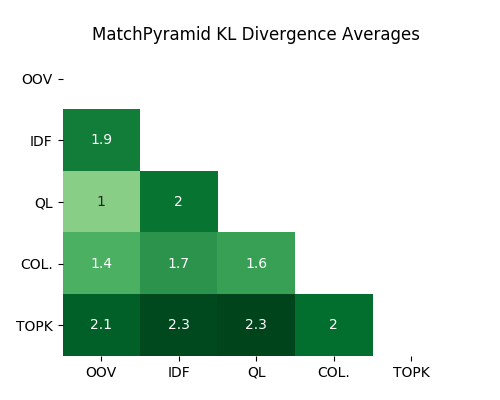
\includegraphics[width=.33\linewidth]{Figures/mp_cos_kl_div.png}\hfill
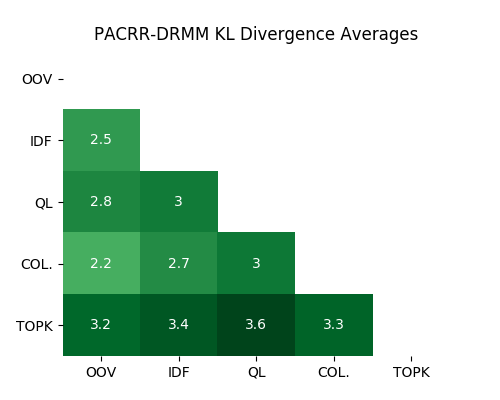
\includegraphics[width=.33\linewidth]{Figures/pacrr_drmm_kl_div.png}
  \caption[Confusion matrices of DeepSHAP background documents comparing Jaccard similarities and Jensen-Shannon divergence.]{Confusion matrices of various DeepSHAP background document methods comparing the overlap in terms of both Jaccard similarities and Jensen-Shannon divergence.}
  \label{fig:shap_confusion_matrices}
\end{figure}


\begin{table}[h]
    \centering
    \begin{tabular}{cccccc}
        \toprule
        LIME & OOV & IDF & QL & COL. & TOPK\\
        \midrule
cult & cult & cult & cult & cult & cult \\
style & followers & style & style & black & {\bf numbers} \\
followers & black & followers & elite & fraternities & {\bf english} \\
elite & fraternities & {\bf suspects} & saloon & degenerate & {\bf college} \\
saloon & degenerate & {\bf belong} & {\bf final} & sons & {\bf university} \\
{\bf student} & sons & {\bf reappearing} & march & followers & {\bf fallouts} \\
home & {\bf academic} & household & {\bf friday} & style & {\bf buccaneers} \\
{\bf members} & {\bf american} & black & september & home & {\bf feudings} \\
march & {\bf tried} & fraternities & {\bf arms} & household & {\bf activists} \\
september & household & degenerate & {\bf closed} & {\bf avoid} & {\bf troubles} \\
        \bottomrule
    \end{tabular}
    \caption[Comparison of explanations from LIME and various DeepSHAP methods for an example document with DRMM.]{An example of words selected by LIME and various DeepSHAP methods with the \textsf{DRMM} model for the query {\bf `cult lifestyles'} and document {\bf `FBIS3-843'} which talks about clashes between cult members and student union's activists at a university in Nigeria. {\it Words unique to a particular explanation method are highlighted in bold}.}
    \label{tab:drmm_qualitative_example}
\end{table}

\subsection{RQ2. Accuracy of reference input methods}\label{sec:interpretability_rq2}

\begin{table}
\footnotesize
\centering
\begin{tabular}{lccc} 
 \toprule
 & DRMM & MatchPyramid & PACRR-DRMM \\
 \midrule

%LIME & 1.000 $\pm$ 0.000 & 1.007 $\pm$ 0.084 & 0.999 $\pm$ 0.004\\
%\cmidrule(lr){2-4}

OOV & 1.000 $\pm$ 0.000 & 0.498 $\pm$ 0.087 & 0.125 $\pm$ 0.077\\
% \cmidrule(lr){2-4}

IDF & 0.998 $\pm$ 0.021 & 0.500 $\pm$ 0.087 & 0.196 $\pm$ 0.113\\
% \cmidrule(lr){2-4}

QL std. form. & 0.998 $\pm$ 0.012 & 0.517 $\pm$ 0.083 & 0.205 $\pm$ 0.114\\
% \cmidrule(lr){2-4}

COLLECTION & 0.999 $\pm$ 0.004 & 0.500 $\pm$ 0.087 & 0.164 $\pm$ 0.083\\
% \cmidrule(lr){2-4}

TOPK LIST. & 0.999 $\pm$ 0.006 & 0.518 $\pm$ 0.095 & 0.162 $\pm$ 0.078\\
\bottomrule
 \end{tabular}
 \caption{Comparison of mean and standard deviation of the fraction of terms returned from LIME and DeepSHAP for ROBUST04 hard queries}
\label{tab:queries_diff_mean_std_terms_shap}
\end{table}

To help identify which reference input method is most accurate in explaining a given query-document pair, we compared the LIME explanations for the same against it's corresponding DeepSHAP explanation methods. In general we found that DeepSHAP produces more explanation terms (see Table~\ref{tab:queries_diff_mean_std_terms_shap}) whereas LIME's L1 regularizer constrains the explanations to only the most important terms (10, 20, 30). Additionally, the discrepancy between the explanations can be attributed to LIME being purely \textit{local}, whereas DeepSHAP has some \textit{global} context since it looks at activations for the whole network which may have captured some global patterns. Hence to estimate which reference input surfaces the most `ground truth' explanation terms we only computed recall at top 50 and 100 (by shapley value magnitude) DeepSHAP explanation terms (in Table~\ref{tab:doc_bg_dist_recall}).

\begin{table}[h]
\scalebox{0.6}{
\begin{tabular}{ m{6em}m{2em}m{2em}m{2em}m{2em}m{2em}m{2em}m{2em}m{2em}m{2em}m{2em}m{2em}m{2em}m{2em}m{2em}m{2em}m{2em}m{2em}m{2em}} 
\toprule
 &\multicolumn{6}{c}{DRMM}&\multicolumn{6}{c}{MatchPyramid}&\multicolumn{6}{c}{PACRR-DRMM}\\
 \cmidrule(r){2-7}
 \cmidrule(r){8-13}
 \cmidrule(r){14-19}
 &\multicolumn{2}{c}{top-10} &\multicolumn{2}{c}{top-20}&\multicolumn{2}{c}{top-30} &\multicolumn{2}{c}{top-10}&\multicolumn{2}{c}{top-20}&\multicolumn{2}{c}{top-30}
 &\multicolumn{2}{c}{top-10}&\multicolumn{2}{c}{top-20}&\multicolumn{2}{c}{top-30}\\
 \cmidrule(r){2-3}
 \cmidrule(r){4-5}
 \cmidrule(r){6-7}
 \cmidrule(r){8-9}
 \cmidrule(r){10-11}
 \cmidrule(r){12-13}
 \cmidrule(r){14-15}
 \cmidrule(r){16-17}
 \cmidrule(r){18-19}
 SHAP \newline variants & recall\newline @50  & recall\newline @100 & recall\newline @50  & recall\newline @100 & recall\newline @50  & recall\newline @100 & recall\newline @50  & recall\newline @100 & recall\newline @50  & recall\newline @100 & recall\newline @50  & recall\newline @100 & recall\newline @50  & recall\newline @100  & recall\newline @50  & recall\newline @100 & recall\newline @50  & recall\newline @100\\
 \midrule

OOV & 0.789 & 0.905 & 0.672 & 0.845 & 0.615 & 0.812 & {\bf 0.793} & {\bf 0.843} & {\bf 0.656} & {\bf 0.726} & {\bf 0.566} & {\bf 0.640} & 0.582 & 0.582 & 0.388 & 0.388 & 0.299 & 0.299\\
% \cmidrule(l){2-19}
\addlinespace[1em]

IDF & 0.830 & 0.917 & 0.723 & 0.871 & 0.658 & 0.841 & 0.795 & 0.832 & 0.653 & 0.711 & 0.565 & 0.633 & 0.633 & 0.633 & 0.446 & 0.446 & 0.362 & 0.362\\
% \cmidrule(l){2-19}
\addlinespace[1em]

QL & {\bf 0.894} & {\bf 0.955} & {\bf 0.754} & {\bf 0.892} & {\bf 0.670} & {\bf 0.856} & 0.765 & 0.821 & 0.638 & 0.711 & 0.556 & 0.636 & {\bf 0.643} & {\bf 0.643} & {\bf 0.462} & {\bf 0.462} & {\bf 0.367} & {\bf 0.367}\\
% \cmidrule(l){2-19}
\addlinespace[1em]

% QL inv. rank \newline \textit{lowest} & 0.897 & 0.958 & 0.752 & 0.892 & 0.666 & 0.854 & 0.790 & 0.838 & 0.654 & 0.720 & 0.566 & 0.638 & 0.627 & 0.627 & 0.448 & 0.448 & 0.362 & 0.362\\
% \hline

% IDF-QL \newline \textit{lowest} & 0.893 & 0.957 & 0.749 & 0.892 & 0.664 & 0.854 & 0.790 & 0.838 & 0.654 & 0.720 & 0.566 & 0.638 & 0.627 & 0.627 & 0.448 & 0.448 & 0.362 & 0.362\\
% \hline

% IDF-QL \newline \textit{rand sample of low scores} & 0.900 & 0.952 & 0.756 & 0.885 & 0.679 & 0.857 & 0.762 & 0.824 & 0.630 & 0.711 & 0.546 & 0.634 & 0.643 & 0.643 & 0.458 & 0.458 & 0.367 & 0.367\\
% \hline

COLLECTION & 0.760 & 0.881 & 0.673 & 0.841 & 0.620 & 0.815 & 0.783 & 0.824 & 0.639 & 0.709 & 0.552 & 0.630 & 0.621 & 0.621 & 0.429 & 0.429 & 0.343 & 0.343\\
% \cmidrule(l){2-19}
\addlinespace[1em]

TOPK LIST. & 0.639 & 0.821 & 0.606 & 0.794 & 0.578 & 0.788 & 0.759 & 0.811 & 0.624 & 0.702 & 0.545 & 0.627 & 0.625 & 0.625 & 0.425 & 0.425 & 0.340 & 0.340\\
\bottomrule

 \end{tabular}}
 \caption[Comparison of recall measures at top-k terms from DeepSHAP against ground-truth terms from LIME.]{Comparison of recall measures at \textit{top-k} (50, 100) terms from DeepSHAP against the \textit{top-k} (10, 20, 30) ground-truth terms from LIME for ROBUST04 hard queries}
\label{tab:doc_bg_dist_recall}
\end{table}

The first interesting insight is that some NRMs are easier to explain whereas others are more difficult. PACRR-DRMM consistently has a recall less than $0.7$ whereas the DeepSHAP explanations of DRMM effectively capture almost all of the LIME explanation terms. When comparing reference input variants within each NRM we find that there is no consistent winner. For DRMM, QL is the best which indicates that sampling terms which are relatively generic for this query in particular is a better `background image' than sampling generic words from the collection (IDF). 

In the case of MatchPyramid, TOPK LIST is the worst performing but it is more difficult to distinguish between the approaches here. The best approach surprisingly is OOV. This can be attributed to how MatchPyramid treats OOV terms. The OOV token is represented by an all-zeros embedding vector that is used for padding the input interaction matrix whereas in DRMM, OOV tokens are filtered out. These preprocessing considerations prove to be crucial when determining the right input reference. Moving on to PACRR-DRMM, we once again find that QL is the best method even though DeepSHAP struggles to find all the LIME terms. It struggles to find more LIME terms because the number of explanation terms returned from DeepSHAP for PACRR-DRMM is only about a small fraction (0.2) of the document. We have left the investigation of why the number of explanation terms returned by DeepSHAP varies based on different NRMs for future work. In Table~\ref{tab:doc_bg_dist_recall_no_q_terms}, we show that we get similar insights as discussed above even if we filter out the query terms from the explanation terms returned from both LIME and SHAP.

\begin{table}[h]
\scalebox{0.6}{
\begin{tabular}{ m{6em}m{2em}m{2em}m{2em}m{2em}m{2em}m{2em}m{2em}m{2em}m{2em}m{2em}m{2em}m{2em}m{2em}m{2em}m{2em}m{2em}m{2em}m{2em} } 
\toprule
 &\multicolumn{6}{c}{DRMM}&\multicolumn{6}{c}{MatchPyramid}&\multicolumn{6}{c}{PACRR-DRMM}\\
 \cmidrule(r){2-7}
 \cmidrule(r){8-13}
 \cmidrule(r){14-19}
 &\multicolumn{2}{c}{top-10} &\multicolumn{2}{c}{top-20}&\multicolumn{2}{c}{top-30} &\multicolumn{2}{c}{top-10}&\multicolumn{2}{c}{top-20}&\multicolumn{2}{c}{top-30}
 &\multicolumn{2}{c}{top-10}&\multicolumn{2}{c}{top-20}&\multicolumn{2}{c}{top-30}\\
 \cmidrule(r){2-3}
 \cmidrule(r){4-5}
 \cmidrule(r){6-7}
 \cmidrule(r){8-9}
 \cmidrule(r){10-11}
 \cmidrule(r){12-13}
 \cmidrule(r){14-15}
 \cmidrule(r){16-17}
 \cmidrule(r){18-19}
 SHAP \newline variants & recall\newline @50  & recall\newline @100 & recall\newline @50  & recall\newline @100 & recall\newline @50  & recall\newline @100 & recall\newline @50  & recall\newline @100 & recall\newline @50  & recall\newline @100 & recall\newline @50  & recall\newline @100 & recall\newline @50  & recall\newline @100  & recall\newline @50  & recall\newline @100 & recall\newline @50  & recall\newline @100\\
 \midrule

% OOV \newline w padding & 0.762 & 0.888 & 0.654 & 0.836 & 0.603 & 0.805 & 0.762 & 0.813 & 0.633 & 0.703 & 0.548 & 0.620 & 0.475 & 0.475 & 0.316 & 0.316 & 0.248 & 0.248\\
% \hline

OOV & 0.762 & 0.888 & 0.654 & 0.836 & 0.603 & 0.805 & \textbf{0.762} & \textbf{0.812} & \textbf{0.633} & \textbf{0.702} & \textbf{0.548} & \textbf{0.619} & 0.472 & 0.472 & 0.315 & 0.315 & 0.245 & 0.245\\
\addlinespace[1em]

IDF & 0.796 & 0.902 & 0.702 & 0.863 & 0.645 & 0.836 & 0.759 & 0.800 & 0.628 & 0.685 & 0.545 & 0.612 & 0.538 & 0.538 & 0.380 & 0.380 & 0.314 & 0.314\\
\addlinespace[1em]

QL std. form. & \textbf{0.874} & \textbf{0.945} & \textbf{0.737} & \textbf{0.884} & \textbf{0.657} & \textbf{0.851} & 0.719 & 0.782 & 0.609 & 0.684 & 0.536 & 0.614 & \textbf{0.552} & \textbf{0.552} & \textbf{0.399} & \textbf{0.399} & \textbf{0.319} & \textbf{0.319}\\
\addlinespace[1em]

% QL inv. rank \newline \textit{lowest} & 0.878 & 0.951 & 0.738 & 0.885 & 0.654 & 0.849 & 0.751 & 0.805 & 0.626 & 0.694 & 0.546 & 0.617 & 0.529 & 0.529 & 0.383 & 0.383 & 0.314 & 0.314\\
% \hline

% IDF-QL \newline \textit{lowest} & 0.873 & 0.950 & 0.734 & 0.885 & 0.653 & 0.849 & 0.751 & 0.805 & 0.626 & 0.694 & 0.546 & 0.617 & 0.529 & 0.529 & 0.383 & 0.383 & 0.314 & 0.314\\
% \hline

% IDF-QL \newline \textit{rand sample of low scores} & 0.882 & 0.943 & 0.736 & 0.878 & 0.667 & 0.853 & 0.718 & 0.789 & 0.602 & 0.685 & 0.527 & 0.613 & 0.552 & 0.552 & 0.394 & 0.394 & 0.319 & 0.319\\
% \hline

COLLECTION & 0.721 & 0.864 & 0.654 & 0.832 & 0.609 & 0.811 & 0.741 & 0.788 & 0.611 & 0.682 & 0.532 & 0.607 & 0.524 & 0.524 & 0.362 & 0.362 & 0.292 & 0.292\\
\addlinespace[1em]

TOPK LIST. & 0.601 & 0.804 & 0.588 & 0.786 & 0.568 & 0.783 & 0.715 & 0.776 & 0.596 & 0.676 & 0.524 & 0.606 & 0.529 & 0.529 & 0.357 & 0.357 & 0.289 & 0.289\\
\bottomrule

 \end{tabular}}
\caption[Comparison of recall measures at top-k terms from DeepSHAP against ground-truth terms from LIME \textit{not including query terms}.]{Comparison of recall measures at \textit{top-k} (50, 100) terms from DeepSHAP against the \textit{top-k} (10, 20, 30) ground-truth terms from LIME for ROBUST04 hard queries; {\bf From both sets of terms we ignore the query terms}}
\label{tab:doc_bg_dist_recall_no_q_terms}
\end{table}

\subsection{RQ3. Effect of reference query distribution}\label{sec:interpretability_rq3}

In order to understand the effect of using a reference query input distribution along with the different reference document methods, we construct a reference query input by sampling words that have low IDF scores from the collection. We evaluate the DeepSHAP explanations by computing recall at top 50 and 100 with respect to `ground truth' terms (in Table~\ref{tab:q_dist_doc_bg_dist_recall}) as in section~\ref{sec:interpretability_rq2}.

\begin{table}[h]
\scalebox{0.6}{
\begin{tabular}{ m{6em}m{2em}m{2em}m{2em}m{2em}m{2em}m{2em}m{2em}m{2em}m{2em}m{2em}m{2em}m{2em}m{2em}m{2em}m{2em}m{2em}m{2em}m{2em} } 
\toprule
 &\multicolumn{6}{c}{DRMM}&\multicolumn{6}{c}{MatchPyramid}&\multicolumn{6}{c}{PACRR-DRMM}\\
 \cmidrule(r){2-7}
 \cmidrule(r){8-13}
 \cmidrule(r){14-19}
 &\multicolumn{2}{c}{top-10} &\multicolumn{2}{c}{top-20}&\multicolumn{2}{c}{top-30} &\multicolumn{2}{c}{top-10}&\multicolumn{2}{c}{top-20}&\multicolumn{2}{c}{top-30}
 &\multicolumn{2}{c}{top-10}&\multicolumn{2}{c}{top-20}&\multicolumn{2}{c}{top-30}\\
 \cmidrule(r){2-3}
 \cmidrule(r){4-5}
 \cmidrule(r){6-7}
 \cmidrule(r){8-9}
 \cmidrule(r){10-11}
 \cmidrule(r){12-13}
 \cmidrule(r){14-15}
 \cmidrule(r){16-17}
 \cmidrule(r){18-19}
 SHAP \newline variants & recall\newline @50  & recall\newline @100 & recall\newline @50  & recall\newline @100 & recall\newline @50  & recall\newline @100 & recall\newline @50  & recall\newline @100 & recall\newline @50  & recall\newline @100 & recall\newline @50  & recall\newline @100 & recall\newline @50  & recall\newline @100  & recall\newline @50  & recall\newline @100 & recall\newline @50  & recall\newline @100\\
 \midrule
 %\hline\hline

OOV & 0.783 & 0.903 & 0.662 & 0.846 & 0.604 & 0.815 & \textbf{0.789} & \textbf{0.840} & \textbf{0.658} & \textbf{0.730} & \textbf{0.568} & \textbf{0.648} & 0.565 & 0.565 & 0.378 & 0.378 & 0.293 & 0.293\\
\addlinespace[1em]

IDF & 0.885 & 0.948 & 0.751 & 0.897 & 0.664 & 0.858 & 0.754 & 0.813 & 0.627 & 0.712 & 0.553 & 0.643 & 0.646 & 0.646 & 0.459 & 0.459 & 0.372 & 0.372\\
\addlinespace[1em]

QL std. form. & \textbf{0.891} & \textbf{0.954} & \textbf{0.760} & \textbf{0.892} & \textbf{0.676} & \textbf{0.861} & 0.746 & 0.811 & 0.621 & 0.707 & 0.541 & 0.637 & \textbf{0.645} & \textbf{0.645} & \textbf{0.463} & \textbf{0.463} & \textbf{0.380} & \textbf{0.380}\\
\addlinespace[1em]

COLLECTION & 0.824 & 0.901 & 0.699 & 0.850 & 0.640 & 0.821 & 0.756 & 0.815 & 0.626 & 0.707 & 0.545 & 0.633 & 0.613 & 0.613 & 0.422 & 0.422 & 0.335 & 0.335\\
\addlinespace[1em]

TOPK LIST. & 0.818 & 0.907 & 0.698 & 0.857 & 0.634 & 0.827 & 0.746 & 0.803 & 0.619 & 0.695 & 0.540 & 0.622 & 0.610 & 0.610 & 0.418 & 0.418 & 0.334 & 0.334\\

\bottomrule
 \end{tabular}}
\caption[Comparison of recall measures at top-k terms from DeepSHAP using query distribution against ground-truth terms from LIME.]{Comparison of recall measures at \textit{top-k} (50, 100) terms from DeepSHAP using also query distribution sampled from low IDF scores against the \textit{top-k} (10, 20, 30) ground-truth terms from LIME for ROBUST04 hard queries}
\label{tab:q_dist_doc_bg_dist_recall}
\end{table}

Similar to the insights described in section~\ref{sec:interpretability_rq2}, we see that the best performing approaches across each of the models are the same--DRMM (QL), MatchPyramid (OOV) and PACRR-DRMM (QL). Thus, using a reference query input distribution doesn't effect the best performing reference document input variants within each NRM. However, for DRMM we observe that it is now hard to distinguish between various approaches which is different from the insights in Table~\ref{tab:doc_bg_dist_recall}. This could be because of the low activations through the attention network in DRMM from the query reference input due to the use of irrelevant words sampled from IDF. But we don't see such differences in MatchPyramid and PACRR-DRMM, as it was already difficult to distinguish between the approaches when the reference query input was fixed and also these two models don't have an attention network.


% \begin{table}
% \centering
% % \scalebox{0.8}{
% \begin{tabular}{ m{7em}m{2em}m{2em}m{2.8em}m{2em}m{2em}m{2.8em}m{2em}m{2em}m{2.8em}} 
%  \toprule
%  &\multicolumn{3}{c}{DRMM}&\multicolumn{3}{c}{MatchPyramid}&\multicolumn{3}{c}{PACRR-DRMM}\\
%  \cmidrule(lr){2-4}
%  \cmidrule(lr){5-7}
%  \cmidrule(lr){8-10}
%  SHAP variants & recall\newline pos & recall\newline neg & jaccard & recall\newline pos & recall\newline neg & jaccard & recall\newline pos & recall\newline neg & jaccard\\
%  \midrule
% %  OOV \newline w padding & 0.602 & 0.601 & 0.176 & 0.185 & 0.263 & 0.467 & 0.477 & 0.148 & 0.159 & 0.281 & 0.329 & 0.398 & 0.190 & 0.211 & 0.256\\
% % \hline

% OOV & 0.602 & 0.176 & 0.263 & 0.468 & 0.148 & 0.281 & 0.327 & 0.193 & 0.257\\

% IDF \textit{lowest} & 0.633 & 0.126 & 0.283 & 0.492 & 0.154 & 0.284 & 0.333 & 0.162 & 0.230\\

% QL std. form. \textit{lowest} & 0.630 & 0.161 & 0.294 & 0.453 & 0.152 & 0.268 & 0.319 & 0.134 & 0.229\\

% % QL inv. rank \newline \textit{lowest} & 0.653 & 0.653 & 0.213 & 0.244 & 0.302 & 0.478 & 0.490 & 0.157 & 0.166 & 0.279 & 0.331 & 0.342 & 0.143 & 0.150 & 0.238\\
% % \hline

% % IDF-QL \newline \textit{lowest} & 0.653 & 0.653 & 0.210 & 0.240 & 0.301 & 0.478 & 0.490 & 0.157 & 0.166 & 0.279 & 0.331 & 0.342 & 0.143 & 0.150 & 0.238\\
% % \hline

% % IDF-QL \newline \textit{rand sample of low scores} & 0.673 & 0.673 & 0.165 & 0.207 & 0.311 & 0.444 & 0.456 & 0.138 & 0.152 & 0.265 & 0.333 & 0.340 & 0.149 & 0.152 & 0.228\\
% % \hline

% COLLECTION \textit{rand doc} & 0.545 & 0.085 & 0.270 & 0.456 & 0.142 & 0.264 & 0.326 & 0.150 & 0.237\\

% TOPK LIST. \textit{rand doc from bottom} & 0.356 & 0.107 & 0.223 & 0.436 & 0.142 & 0.262 & 0.327 & 0.155 & 0.244\\
% \bottomrule
%  \end{tabular}
% %  }
% \caption{Comparison of overlap measures between \textit{top-10} terms returned from LIME and SHAP based on different background samples for ROBUST04 difficult queries (50)}
% \label{table_diff_10_terms}
% \end{table}

% \subsection{RQ4.}
% \begin{table}
% \scalebox{0.78}{
% \begin{tabular}{m{6em}m{4em}m{4em}m{4em}m{4em}m{4em}m{4em}m{4em}m{4em}m{4em}} 
%  \toprule
%  &\multicolumn{3}{c}{DRMM}&\multicolumn{3}{c}{MatchPyramid}&\multicolumn{3}{c}{PACRR-DRMM}\\
%  \cmidrule(r){2-4}
%  \cmidrule(r){5-7}
%  \cmidrule(r){8-10}
%   & MRR & Kendall's $\uptau@10$ & Kendall's $\uptau@1000$ & MRR & Kendall's $\uptau@10$ & Kendall's $\uptau@all$ & MRR & Kendall's $\uptau@10$ & Kendall's $\uptau@1000$ \\
%  \midrule
% LIME & \textbf{0.701} & 0.224 & \textbf{0.379} & \textbf{0.470} & 0.181 & 0.240 & 0.880 & 0.361 & \textbf{0.476}\\
% % \cmidrule(lr){2-10}
% SHAP\\
% \cmidrule(lr){1-1}
% % OOV w padding & 0.545 & 0.203 & \textbf{0.379} & 0.334 & 0.188 & \textbf{0.280} & 0.878 & 0.320 & 0.344\\
% % \cmidrule(lr){2-10}

% OOV & 0.545 & 0.203 & {\bf 0.379} & 0.376 & 0.211 & {\bf 0.276} & 0.864 & 0.332 & 0.352\\
% % \cmidrule(lr){2-10}

% IDF & 0.614 & 0.238 & 0.354 & 0.399 & 0.181 & 0.243 & 0.932 & 0.345 & 0.377\\
% % \cmidrule(lr){2-10}

% QL std. form. & 0.592 & 0.227 & 0.358 & 0.397 & 0.175 & 0.261 & 0.933 & 0.370 & 0.385\\
% % \cmidrule(lr){2-10}

% %QL inv. rank \textit{lowest} & 0.512 & 0.211 & 0.351 & 0.327 & \textbf{0.240} & 0.273 & 0.928 & 0.331 & 0.395\\
% %\cmidrule(lr){2-10}

% % IDF-QL \textit{lowest} & 0.512 & 0.211 & 0.351 & 0.327 & \textbf{0.240} & 0.273 & 0.928 & 0.331 & 0.395\\
% % \cmidrule(lr){2-10}

% %IDF-QL \textit{rand sample of low scores} & 0.560 & 0.214 & 0.356 & 0.340 & 0.207 & 0.245 & 0.932 & 0.331 & 0.382\\
% %\cmidrule(lr){2-10}

% COLLECTION  & 0.548 & 0.221 & 0.340 & 0.382 & 0.189 & 0.250 & \textbf{0.953} & \textbf{0.391} & \textbf{0.399}\\
% % \cmidrule(lr){2-10}

% TOPK LIST. & \textbf{0.676} & \textbf{0.256} & 0.296 & \textbf{0.408} & 0.183 & 0.253 & 0.923 & 0.373 & 0.394\\

% \bottomrule
% \end{tabular}}
% \caption{Comparison of rank differences between new ranking with the {\it top-5} LIME or {\it top-5} DeepSHAP terms from the {\it top-1} doc as queries to the black-box ranker and the original black-box ranking using ROBUST04 hard queries (50); the highest measures in each column and highest among the SHAP variants are marked in {\bf bold}}
% \label{tab:rank_diff_lime_shap}
% \end{table}




% \begin{table}
% \caption{Comparison of different model performances of LIME across the various neural ranking models}
% \label{tab:lime_model_performances}
% \scalebox{0.7}{
% \begin{tabular}{lcccccccc} 
%  \toprule
%  &\multicolumn{4}{c}{Linear Regression} &\multicolumn{4}{c}{MLP}\\
%  \cmidrule(lr){2-5}
%  \cmidrule(lr){6-9}
%  NRM & TRAIN MSE & TEST MSE & TRAIN ACC & TEST ACC & TRAIN MSE & TEST MSE & TRAIN ACC & TEST ACC\\
%  \midrule
%  DRMM & 0.00631 & 0.00633 & 0.92662 & 0.92654 & 0.00419 & 0.00428 & 0.94768 & 0.94789\\
%  MatchPyramid & 0.01827 & 0.01839 & 0.90367 & 0.90387 & 0.00980 & 0.01030 & 0.92558 & 0.92445\\
%  PACRR-DRMM & 0.00165 & 0.00160 & 0.98857 & 0.98980 & 0.00339 & 0.00356 & 0.98745 & 0.98662\\
% \bottomrule
% \end{tabular}}
% \end{table} 
% Chapter Template

\chapter{Conclusion} % Main chapter title

\label{Chapter6} % Change X to a consecutive number; for referencing this chapter elsewhere, use \ref{ChapterX}

\lhead{Chapter 6. \emph{Conclusion}} % Change X to a consecutive number; this is for the header on each page - perhaps a shortened title

In this thesis, we successfully trained various \textit{interaction-based} neural ranking models on the standard TREC newswire collection (Robust04) and reproduced results that had a similar retrieval effectiveness or a retrieval performance close to what was reported in the papers across all the evaluation metrics. The few differences that we observed in our experiments were mainly due to the lack of information regarding the exact splits of the data that were used for cross-validation, or the exact hyper-parameters used to tune the model along with the amount of data that was sampled (number of iterations or epochs for which the model was trained, number of query-document pairs sampled) or how the ranking pairs were sampled from the relevance judgements. The two neural ranking models--PACRR-DRMM and NPRF-DRMM for which the above data was reported or shared, helped us train models that had retrieval effectiveness exactly as reported in the paper. We also investigated the reproducibility of DSSM, a \textit{representation-based} neural ranking model which has been shown to perform well only on large-scale click-through proprietary datasets. We had  tried various approaches that included pre-training the triletter representations using the target corpus, or weak supervision using AOL queries to generate a large set of training data and a combination of both, but couldn't train an effective model which was also highlighted in a parallel study~\citep{nie_ictir_18}. In the future, we would like to investigate in detail as to why we were not able train an effective model on the Robust04 newswire collection, and if given a large public dataset (MS-MARCO) can we train an effective DSSM model. %even if it was shown previously that \textit{representation-based} approaches can be trained effectively with weak supervision~\citep{Dehghani_sigir17}. 
This thesis  covers an extensive survey of the existing neural ranking approaches in the literature as well (Chapter~\ref{Chapter2}).

In this thesis, we also investigated the applicability of existing \textit{model-introspective} interpretability approaches in ML, such as, DeepSHAP for explaining the decisions of complex neural ranking models--\textit{why} a particular document was considered relevant for the query. We suggested several reference input methods for DeepSHAP that take into account the unique semantics of document ranking and relevance in IR. Through quantitative experiments we found that it is indeed sensitive to the reference input. The distinct lack of overlap in most cases was surprising but in line with recent works on the lack of robustness in interpretability approaches~\citep{Ghorbani2017}. We also tried to evaluate which reference method is more accurate by comparing against a \textit{model-agnostic} approach LIME. Here we found that the reference input method selection is highly dependent on the neural ranking model at hand. We believe that this work exposes new problems when dealing with model introspective interpretability for NRMs. 

A worthwhile endeavor will be to investigate new approaches that explicitly take into account the discreteness of text and the model's preprocessing choices when generating explanations. It would also be interesting to consider how we can answer the following ranking questions to help the user understand the underlying neural ranking model better:

\begin{itemize}
    \item \textsf{What is the intent of the query encoded by the neural ranking model?} -- Could we simply aggregate the term weights returned by DeepSHAP from top-\textit{k} results and pick the top-\textit{n} words to indicate intent of the query.
    \item \textsf{Why a particular document $d_A$ is ranked higher than another document $d_B$ in the ranked list?} -- Could we construct a `reference' input from the distribution of terms in the lower ranked document $d_B$ that would help pick terms which are different or unique that explain the higher relevance of $d_A$.
\end{itemize}
 
% \begin{table}
\scalebox{0.65}{
\begin{tabular}{ |m{6em}|m{2em}|m{2em}|m{2em}|m{2em}|m{2.8em}||m{2em}|m{2em}|m{2em}|m{2em}|m{2.8em}||m{2em}|m{2em}|m{2em}|m{2em}|m{2.8em}|| } 
 \hline
 &\multicolumn{5}{|c||}{DRMM}&\multicolumn{5}{|c||}{MatchPyramid}&\multicolumn{5}{|c|}{PACRR-DRMM}\\
 \hline
 SHAP \newline variants & recall\newline pos & prec\newline pos & recall\newline neg & prec\newline neg  & jaccard & recall\newline pos & prec\newline pos & recall\newline neg & prec\newline neg & jaccard & recall\newline pos & prec\newline pos & recall\newline neg & prec\newline neg &
 jaccard\\
 \hline\hline
 OOV \newline w padding & 0.712 & 0.529 & 0.544 & 0.732
  & 0.988 & 0.334 & 0.558 & 0.220 & 0.519 & 0.449 & 0.076 & 0.666 & 0.070 & 0.480 & 0.118\\
 \hline
 
 OOV w/o padding & 0.712 & 0.529 & 0.544 & 0.732 & 0.988 & 0.333 & 0.559 & 0.220 & 0.518 & 0.448 & 0.075 & 0.667 & 0.069 & 0.477 & 0.116\\ 
 \hline
 
 IDF \newline \textit{lowest} & 0.685 & 0.476 & 0.444 & 0.674 & 0.985 & 0.329 & 0.560 & 0.227 & 0.530 & 0.453 & 0.111 & 0.631 & 0.099 & 0.455 & 0.180\\
 \hline
 
 QL std. form.\newline \textit{lowest} & 0.769 & 0.443 & 0.303 & 0.626 & 0.986 & 0.338 & 0.548 & 0.231 & 0.531 & 0.468 & 0.113 & 0.585 & 0.101 & 0.453 & 0.187\\
 \hline
 
 QL inv. rank \newline \textit{lowest} & 0.841 & 0.495 & 0.380 & 0.790 & 0.987 & 0.326 & 0.560 & 0.242 & 0.541 & 0.458 & 0.105 & 0.589 & 0.100 & 0.448 & 0.181\\
 \hline
 
 IDF-QL \newline \textit{lowest} & 0.841 & 0.494 & 0.378 & 0.784 & 0.987 & 0.326 & 0.560 & 0.242 & 0.541 & 0.458 & 0.105 & 0.589 & 0.100 & 0.448 & 0.181\\ 
 \hline
 
 IDF-QL \newline \textit{rand sample of low scores} & 0.798 & 0.448 & 0.290 & 0.671 & 0.985 & 0.341 & 0.543 & 0.236 & 0.533 & 0.475 & 0.119 & 0.618 & 0.103 & 0.461 & 0.185\\ 
 \hline
 
 COLLECTION \newline \textit{rand doc} & 0.673 & 0.525 & 0.429 & 0.534 & 0.987 & 0.309 & 0.560 & 0.240 & 0.524 & 0.451 & 0.096 & 0.630 & 0.080 & 0.452 & 0.148\\ 
 \hline
 
 TOPK LIST. \newline \textit{rand doc from bottom} & 0.583 & 0.514 & 0.482 & 0.567 & 0.987 & 0.318 & 0.557 & 0.252 & 0.529 & 0.466 & 0.094 & 0.618 & 0.079 & 0.454 & 0.147\\ 
 \hline
\end{tabular}}
\caption{Comparison of overlap measures between LIME and SHAP based on different background samples for ROBUST04 difficult queries (50)}
\label{table_diff_all_terms}
\end{table}

% ------------------------------------------------
\begin{table}
\scalebox{0.65}{
\begin{tabular}{ |m{6em}|m{2em}|m{2em}|m{2em}|m{2em}|m{2.8em}||m{2em}|m{2em}|m{2em}|m{2em}|m{2.8em}||m{2em}|m{2em}|m{2em}|m{2em}|m{2.8em}|| } 
 \hline
 &\multicolumn{5}{|c||}{DRMM}&\multicolumn{5}{|c||}{MatchPyramid}&\multicolumn{5}{|c|}{PACRR-DRMM}\\
 \hline
 SHAP \newline variants & recall\newline pos & prec\newline pos & recall\newline neg & prec\newline neg  & jaccard & recall\newline pos & prec\newline pos & recall\newline neg & prec\newline neg & jaccard & recall\newline pos & prec\newline pos & recall\newline neg & prec\newline neg &
 jaccard\\
 \hline\hline
 OOV \newline w padding & 0.723 & 0.518 & 0.523 & 0.738 & 0.999 & 0.330 & 0.581 & 0.227 & 0.501 & 0.455 & 0.073 & 0.670 & 0.063 & 0.426 & 0.117\\
 \hline
 
 OOV w/o padding & 0.723 & 0.518 & 0.523 & 0.738 & 0.999 & 0.330 & 0.581 & 0.226 & 0.501 & 0.454 & 0.072 & 0.675 & 0.061 & 0.421 & 0.114\\ 
 \hline
 IDF \newline \textit{lowest} & 0.669 & 0.471 & 0.441 & 0.652 & 0.999 & 0.320 & 0.582 & 0.250 & 0.515 & 0.462 & 0.108 & 0.625 & 0.098 & 0.437 & 0.180\\
 \hline
 QL std. form.\newline \textit{lowest} & 0.810 & 0.446 & 0.277 & 0.672 & 0.998 & 0.331 & 0.555 & 0.232 & 0.491 & 0.478 & 0.118 & 0.596 & 0.095 & 0.434 & 0.189\\
 \hline
 QL inv. rank \newline \textit{lowest} & 0.849 & 0.488 & 0.360 & 0.792 & 0.999 & 0.319 & 0.570 & 0.247 & 0.503 & 0.468 & 0.107 & 0.593 & 0.096 & 0.443 & 0.181\\
 \hline
 IDF-QL \newline \textit{lowest} & 0.849 & 0.488 & 0.360 & 0.792 & 0.999 & 0.319 & 0.570 & 0.247 & 0.503 & 0.468 & 0.107 & 0.593 & 0.096 & 0.443 & 0.181\\ 
 \hline
 IDF-QL \newline \textit{rand sample of low scores} & 0.811 & 0.445 & 0.272 & 0.679 & 0.998 & 0.334 & 0.551 & 0.241 & 0.499 & 0.484 & 0.116 & 0.602 & 0.103 & 0.441 & 0.193\\ 
 \hline
 COLLECT. \newline \textit{rand doc} & 0.652 & 0.507 & 0.452 & 0.561 & 0.999 & 0.315 & 0.575 & 0.251 & 0.501 & 0.467 & 0.103 & 0.624 & 0.083 & 0.428 & 0.161\\ 
 \hline
 TOPK LIST. \newline \textit{rand doc from bottom} & 0.622 & 0.483 & 0.427 & 0.551 & 0.999 & 0.311 & 0.569 & 0.254 & 0.499 & 0.469 & 0.091 & 0.632 & 0.078 & 0.430 & 0.145\\ 
 \hline
\end{tabular}}
\caption{Comparison of overlap measures between LIME and SHAP based on different background samples for ROBUST04 non-difficult queries (50)}
\label{table_norm_all_terms}
\end{table}

% ------------------------------------------------
\begin{table}
\scalebox{0.65}{
\begin{tabular}{ |m{6em}|m{2em}|m{2em}|m{2em}|m{2em}|m{2.8em}||m{2em}|m{2em}|m{2em}|m{2em}|m{2.8em}||m{2em}|m{2em}|m{2em}|m{2em}|m{2.8em}|| } 
 \hline
 &\multicolumn{5}{|c||}{DRMM}&\multicolumn{5}{|c||}{MatchPyramid}&\multicolumn{5}{|c|}{PACRR-DRMM}\\
 \hline
 SHAP \newline variants & recall\newline pos & prec\newline pos & recall\newline neg & prec\newline neg  & jaccard & recall\newline pos & prec\newline pos & recall\newline neg & prec\newline neg & jaccard & recall\newline pos & prec\newline pos & recall\newline neg & prec\newline neg &
 jaccard\\
 \hline\hline

OOV \newline w padding & 0.857 & 0.581 & 0.584 & 0.321 & 0.367 & 0.513 & 0.448 & 0.296 & 0.234 & 0.326 & 0.199 & 0.443 & 0.144 & 0.275 & 0.206\\
\hline

%OOV w/o padding & 0.857 & 0.581 & 0.584 & 0.321 & 0.367 & 0.512 & 0.451 & 0.297 & 0.235 & 0.326 & 0.197 & 0.443 & 0.143 & 0.276 & 0.205\\
% \hline

IDF \newline \textit{lowest} & 0.787 & 0.539 & 0.446 & 0.279 & 0.365 & 0.497 & 0.447 & 0.318 & 0.245 & 0.328 & 0.235 & 0.334 & 0.164 & 0.214 & 0.226\\
\hline

QL std. form.\newline \textit{lowest} & 0.836 & 0.563 & 0.334 & 0.277 & 0.374 & 0.500 & 0.432 & 0.297 & 0.237 & 0.322 & 0.235 & 0.304 & 0.167 & 0.212 & 0.230\\
\hline

%QL inv. rank \newline \textit{lowest} & 0.935 & 0.621 & 0.438 & 0.386 & 0.380 & 0.500 & 0.453 & 0.322 & 0.251 & 0.329 & 0.229 & 0.327 & 0.157 & 0.200 & 0.223\\
% \hline

%IDF-QL \newline \textit{lowest} & 0.935 & 0.619 & 0.435 & 0.381 & 0.378 & 0.500 & 0.453 & 0.322 & 0.251 & 0.329 & 0.229 & 0.327 & 0.157 & 0.200 & 0.223\\
% \hline

%IDF-QL \newline \textit{rand sample of low scores} & 0.873 & 0.594 & 0.330 & 0.307 & 0.368 & 0.494 & 0.425 & 0.303 & 0.232 & 0.311 & 0.246 & 0.330 & 0.167 & 0.213 & 0.224\\
% \hline

COLLECTION \newline \textit{rand doc} & 0.813 & 0.496 & 0.437 & 0.170 & 0.338 & 0.477 & 0.439 & 0.321 & 0.233 & 0.316 & 0.227 & 0.373 & 0.141 & 0.224 & 0.210\\
\hline

TOPK LIST. \newline \textit{rand doc from bottom} & 0.667 & 0.356 & 0.489 & 0.213 & 0.318 & 0.471 & 0.428 & 0.325 & 0.230 & 0.309 & 0.224 & 0.360 & 0.144 & 0.232 & 0.215\\
\hline
 \end{tabular}}
\caption{Comparison of overlap measures between \textit{top-20} terms returned from LIME and SHAP based on different background samples for ROBUST04 difficult queries (50)}
\label{table_diff_20_terms}
\end{table}

% ------------------------------------------------
\begin{table}
\scalebox{0.65}{
\begin{tabular}{ |m{6em}|m{2em}|m{2em}|m{2em}|m{2em}|m{2.8em}||m{2em}|m{2em}|m{2em}|m{2em}|m{2.8em}||m{2em}|m{2em}|m{2em}|m{2em}|m{2.8em}|| } 
 \hline
 &\multicolumn{5}{|c||}{DRMM}&\multicolumn{5}{|c||}{MatchPyramid}&\multicolumn{5}{|c|}{PACRR-DRMM}\\
 \hline
 SHAP \newline variants & recall\newline pos & prec\newline pos & recall\newline neg & prec\newline neg  & jaccard & recall\newline pos & prec\newline pos & recall\newline neg & prec\newline neg & jaccard & recall\newline pos & prec\newline pos & recall\newline neg & prec\newline neg &
 jaccard\\
 \hline\hline
 
OOV \newline w padding & 0.606 & 0.593 & 0.288 & 0.316 & 0.358 & 0.402 & 0.438 & 0.187 & 0.232 & 0.320 & 0.196 & 0.427 & 0.122 & 0.217 & 0.200\\
\hline

% OOV w/o padding & 0.606 & 0.593 & 0.288 & 0.316 & 0.358 & 0.401 & 0.437 & 0.188 & 0.233 & 0.322 & 0.196 & 0.437 & 0.120 & 0.218 & 0.200\\
%\hline

IDF \newline \textit{lowest} & 0.577 & 0.568 & 0.197 & 0.254 & 0.341 & 0.408 & 0.449 & 0.208 & 0.241 & 0.326 & 0.238 & 0.328 & 0.153 & 0.183 & 0.220\\
\hline

QL std. form.\newline \textit{lowest} & 0.603 & 0.592 & 0.189 & 0.289 & 0.354 & 0.377 & 0.401 & 0.182 & 0.220 & 0.314 & 0.253 & 0.310 & 0.141 & 0.174 & 0.219\\
\hline

% QL inv. rank \newline \textit{lowest} & 0.653 & 0.638 & 0.262 & 0.357 & 0.367 & 0.396 & 0.433 & 0.200 & 0.242 & 0.321 & 0.236 & 0.317 & 0.133 & 0.168 & 0.216\\
%\hline

% IDF-QL \newline \textit{lowest} & 0.653 & 0.638 & 0.262 & 0.357 & 0.367 & 0.396 & 0.433 & 0.200 & 0.242 & 0.321 & 0.236 & 0.317 & 0.133 & 0.168 & 0.216\\
%\hline

% IDF-QL \newline \textit{rand sample of low scores} & 0.630 & 0.619 & 0.167 & 0.292 & 0.345 & 0.363 & 0.389 & 0.193 & 0.229 & 0.308 & 0.239 & 0.297 & 0.147 & 0.170 & 0.220\\
%\hline

COLLECTION \newline \textit{rand doc} & 0.526 & 0.519 & 0.149 & 0.201 & 0.327 & 0.389 & 0.429 & 0.196 & 0.232 & 0.312 & 0.230 & 0.337 & 0.131 & 0.180 & 0.205\\
\hline

TOPK LIST. \newline \textit{rand doc from bottom} & 0.367 & 0.360 & 0.144 & 0.191 & 0.293 & 0.376 & 0.416 & 0.190 & 0.227 & 0.309 & 0.229 & 0.378 & 0.133 & 0.192 & 0.204\\
\hline
 \end{tabular}}
\caption{Comparison of overlap measures between \textit{top-20} terms returned from LIME and SHAP based on different background samples for ROBUST04 non-difficult queries (50)}
\label{table_norm_20_terms}
\end{table}

% ------------------------------------------------
\begin{table}
\scalebox{0.65}{
\begin{tabular}{ |m{6em}|m{2em}|m{2em}|m{2em}|m{2em}|m{2.8em}||m{2em}|m{2em}|m{2em}|m{2em}|m{2.8em}||m{2em}|m{2em}|m{2em}|m{2em}|m{2.8em}|| } 
 \hline
 &\multicolumn{5}{|c||}{DRMM}&\multicolumn{5}{|c||}{MatchPyramid}&\multicolumn{5}{|c|}{PACRR-DRMM}\\
 \hline
 SHAP \newline variants & recall\newline pos & prec\newline pos & recall\newline neg & prec\newline neg  & jaccard & recall\newline pos & prec\newline pos & recall\newline neg & prec\newline neg & jaccard & recall\newline pos & prec\newline pos & recall\newline neg & prec\newline neg &
 jaccard\\
 \hline\hline
 OOV \newline w padding & 0.615 & 0.614 & 0.183 & 0.192 & 0.265 & 0.481 & 0.484 & 0.143 & 0.151 & 0.274 & 0.329 & 0.389 & 0.174 & 0.184 & 0.242\\
\hline

%OOV w/o padding & 0.615 & 0.614 & 0.183 & 0.192 & 0.265 & 0.483 & 0.486 & 0.145 & 0.153 & 0.277 & 0.329 & 0.396 & 0.174 & 0.187 & 0.244\\
% \hline

IDF \newline \textit{lowest} & 0.644 & 0.643 & 0.123 & 0.130 & 0.275 & 0.485 & 0.493 & 0.160 & 0.162 & 0.278 & 0.332 & 0.336 & 0.143 & 0.143 & 0.223\\
\hline

QL std. form.\newline \textit{lowest} & 0.681 & 0.681 & 0.149 & 0.181 & 0.297 & 0.462 & 0.463 & 0.134 & 0.141 & 0.267 & 0.335 & 0.337 & 0.127 & 0.128 & 0.212\\
\hline

%QL inv. rank \newline \textit{lowest} & 0.660 & 0.659 & 0.195 & 0.220 & 0.294 & 0.496 & 0.500 & 0.156 & 0.165 & 0.285 & 0.321 & 0.327 & 0.129 & 0.130 & 0.214\\
% \hline

%IDF-QL \newline \textit{lowest} & 0.660 & 0.659 & 0.195 & 0.220 & 0.294 & 0.496 & 0.500 & 0.156 & 0.165 & 0.285 & 0.321 & 0.327 & 0.129 & 0.130 & 0.214\\
% \hline

%IDF-QL \newline \textit{rand sample of low scores} & 0.678 & 0.677 & 0.137 & 0.192 & 0.293 & 0.453 & 0.454 & 0.136 & 0.143 & 0.259 & 0.311 & 0.314 & 0.123 & 0.123 & 0.206\\
% \hline

COLLECTION \newline \textit{rand doc} & 0.606 & 0.605 & 0.099 & 0.116 & 0.272 & 0.474 & 0.476 & 0.141 & 0.147 & 0.271 & 0.317 & 0.341 & 0.131 & 0.137 & 0.221\\
\hline

TOPK LIST. \newline \textit{rand doc from bottom} & 0.399 & 0.399 & 0.082 & 0.097 & 0.215 & 0.450 & 0.455 & 0.147 & 0.154 & 0.268 & 0.331 & 0.362 & 0.147 & 0.154 & 0.230\\
\hline
 \end{tabular}}
\caption{Comparison of overlap measures between \textit{top-10} terms returned from LIME and SHAP based on different background samples for ROBUST04 non-difficult queries (50)}
\label{table_norm_10_terms}
\end{table}

% ------------------------------------------------
\begin{table}
\scalebox{0.65}{
\begin{tabular}{ |m{6em}|m{2em}|m{2em}|m{2em}|m{2em}|m{2.8em}||m{2em}|m{2em}|m{2em}|m{2em}|m{2.8em}||m{2em}|m{2em}|m{2em}|m{2em}|m{2.8em}|| } 
 \hline
 &\multicolumn{5}{|c||}{DRMM}&\multicolumn{5}{|c||}{MatchPyramid}&\multicolumn{5}{|c|}{PACRR-DRMM}\\
 \hline
 SHAP \newline variants & recall\newline pos & prec\newline pos & recall\newline neg & prec\newline neg  & jaccard & recall\newline pos & prec\newline pos & recall\newline neg & prec\newline neg & jaccard & recall\newline pos & prec\newline pos & recall\newline neg & prec\newline neg &
 jaccard\\
 \hline\hline

%OOV \newline w padding & 0.994 & 0.757 & 0.642 & 0.060 & 0.360 & 0.895 & 0.664 & 0.546 & 0.033 & 0.335 & 0.595 & 0.520 & 0.528 & 0.044 & 0.358\\
% \hline

OOV w/o padding & 0.994 & 0.757 & 0.642 & 0.060 & 0.360 & 0.898 & 0.669 & 0.574 & 0.034 & 0.345 & 0.595 & 0.517 & 0.528 & 0.045 & 0.360\\
\hline

IDF \newline \textit{lowest} & 0.964 & 0.767 & 0.422 & 0.045 & 0.374 & 0.895 & 0.694 & 0.636 & 0.055 & 0.369 & 0.624 & 0.494 & 0.500 & 0.021 & 0.311\\
\hline

QL std. form.\newline \textit{lowest} & 0.984 & 0.809 & 0.425 & 0.092 & 0.418 & 0.905 & 0.686 & 0.534 & 0.030 & 0.357 & 0.619 & 0.479 & 0.467 & 0.014 & 0.300\\
\hline

%QL inv. rank \newline \textit{lowest} & 0.996 & 0.764 & 0.486 & 0.101 & 0.381 & 0.905 & 0.691 & 0.610 & 0.044 & 0.372 & 0.611 & 0.498 & 0.442 & 0.012 & 0.320\\
% \hline

%IDF-QL \newline \textit{lowest} & 0.996 & 0.764 & 0.477 & 0.097 & 0.378 & 0.905 & 0.691 & 0.610 & 0.044 & 0.372 & 0.611 & 0.498 & 0.442 & 0.012 & 0.320\\
% \hline

%IDF-QL \newline \textit{rand sample of low scores} & 0.981 & 0.815 & 0.434 & 0.108 & 0.425 & 0.910 & 0.702 & 0.547 & 0.028 & 0.355 & 0.617 & 0.499 & 0.507 & 0.015 & 0.309\\
% \hline

COLLECTION \newline \textit{rand doc} & 0.959 & 0.742 & 0.455 & 0.026 & 0.357 & 0.873 & 0.696 & 0.600 & 0.031 & 0.368 & 0.609 & 0.518 & 0.464 & 0.033 & 0.331\\
\hline

TOPK LIST. \newline \textit{rand doc from bottom} & 0.752 & 0.467 & 0.464 & 0.041 & 0.251 & 0.862 & 0.578 & 0.599 & 0.041 & 0.310 & 0.617 & 0.478 & 0.465 & 0.031 & 0.288\\
\hline
 
 \end{tabular}}
\caption{Comparison of overlap measures between \textit{top} terms based on max difference cutoff returned from LIME and SHAP based on different background samples for ROBUST04 difficult queries (50)}
\label{table_diff_max_terms}
\end{table}

% ------------------------------------------------
\begin{table}
\scalebox{0.65}{
\begin{tabular}{ |m{6em}|m{2em}|m{2em}|m{2em}|m{2em}|m{2.8em}||m{2em}|m{2em}|m{2em}|m{2em}|m{2.8em}||m{2em}|m{2em}|m{2em}|m{2em}|m{2.8em}|| } 
 \hline
 &\multicolumn{5}{|c||}{DRMM}&\multicolumn{5}{|c||}{MatchPyramid}&\multicolumn{5}{|c|}{PACRR-DRMM}\\
 \hline
 SHAP \newline variants & recall\newline pos & prec\newline pos & recall\newline neg & prec\newline neg  & jaccard & recall\newline pos & prec\newline pos & recall\newline neg & prec\newline neg & jaccard & recall\newline pos & prec\newline pos & recall\newline neg & prec\newline neg &
 jaccard\\
 \hline\hline

OOV \newline w padding & 0.740 & 0.740 & 0.057 & 0.059 & 0.361 & 0.661 & 0.661 & 0.038 & 0.038 & 0.344 & 0.529 & 0.535 & 0.072 & 0.075 & 0.369\\
\hline

% OOV w/o padding & 0.740 & 0.740 & 0.057 & 0.059 & 0.361 & 0.653 & 0.653 & 0.033 & 0.033 & 0.343 & 0.537 & 0.545 & 0.073 & 0.076 & 0.374\\
% \hline

IDF \newline \textit{lowest} & 0.780 & 0.780 & 0.072 & 0.073 & 0.396 & 0.708 & 0.708 & 0.063 & 0.063 & 0.379 & 0.510 & 0.510 & 0.053 & 0.056 & 0.331\\
\hline

QL std. form.\newline \textit{lowest} & 0.808 & 0.808 & 0.080 & 0.086 & 0.424 & 0.674 & 0.674 & 0.067 & 0.067 & 0.357 & 0.482 & 0.482 & 0.023 & 0.027 & 0.292\\
\hline

% QL inv. rank \newline \textit{lowest} & 0.788 & 0.788 & 0.097 & 0.105 & 0.403 & 0.716 & 0.716 & 0.069 & 0.069 & 0.375 & 0.504 & 0.504 & 0.040 & 0.042 & 0.335\\
% \hline

% IDF-QL \newline \textit{lowest} & 0.788 & 0.788 & 0.097 & 0.105 & 0.403 & 0.716 & 0.716 & 0.069 & 0.069 & 0.375 & 0.504 & 0.504 & 0.040 & 0.042 & 0.335\\
% \hline

% IDF-QL \newline \textit{rand sample of low scores} & 0.821 & 0.821 & 0.069 & 0.074 & 0.423 & 0.659 & 0.659 & 0.042 & 0.042 & 0.344 & 0.475 & 0.475 & 0.041 & 0.044 & 0.297\\
% \hline

COLLECTION \newline \textit{rand doc} & 0.778 & 0.778 & 0.030 & 0.030 & 0.381 & 0.686 & 0.686 & 0.049 & 0.049 & 0.359 & 0.508 & 0.509 & 0.055 & 0.059 & 0.331\\
\hline

TOPK LIST. \newline \textit{rand doc from bottom} & 0.498 & 0.498 & 0.038 & 0.040 & 0.269 & 0.634 & 0.634 & 0.044 & 0.044 & 0.333 & 0.482 & 0.484 & 0.042 & 0.044 & 0.298\\
\hline
 \end{tabular}}
\caption{Comparison of overlap measures between \textit{top} terms based on max difference cutoff returned from LIME and SHAP based on different background samples for ROBUST04 non-difficult queries (50)}
\label{table_norm_max_diff_terms}
\end{table}

% ------------------------------------------------
\begin{table}
\scalebox{0.55}{
\begin{tabular}{ |m{6em}|m{2.8em}|m{2.8em}|m{2.8em}|m{2.8em}|m{2.8em}||m{2.8em}|m{2.8em}|m{2.8em}|m{2.8em}|m{2.8em}||m{2.8em}|m{2.8em}|m{2.8em}|m{2.8em}|m{2.8em}|| } 
 \hline
 &\multicolumn{5}{|c||}{DRMM}&\multicolumn{5}{|c||}{MatchPyramid}&\multicolumn{5}{|c|}{PACRR-DRMM}\\
 \hline
 SHAP \newline variants & recall\newline @10 & recall\newline @20 & recall\newline @30 & recall\newline @40  & recall\newline @50 & recall\newline @10 & recall\newline @20 & recall\newline @30 & recall\newline @40  & recall\newline @50 & recall\newline @10 & recall\newline @20 & recall\newline @30 & recall\newline @40  & recall\newline @50\\
 \hline\hline

% OOV \newline w padding & 0.255 & 0.400 & 0.499 & 0.573 & 0.633 & 0.255 & 0.404 & 0.494 & 0.556 & 0.600 & 0.253 & 0.360 & 0.381 & 0.384 & 0.384\\
% \hline

OOV w/o padding & 0.255 & 0.400 & 0.499 & 0.573 & 0.633 & 0.256 & 0.405 & 0.492 & 0.556 & 0.598 & 0.257 & 0.360 & 0.380 & 0.382 & 0.382\\
\hline

IDF \newline \textit{lowest} & 0.258 & 0.418 & 0.514 & 0.588 & 0.646 & 0.262 & 0.410 & 0.502 & 0.564 & 0.608 & 0.214 & 0.351 & 0.419 & 0.439 & 0.442\\
\hline

QL std. form.\newline \textit{lowest} & 0.284 & 0.426 & 0.523 & 0.591 & 0.652 & 0.252 & 0.391 & 0.487 & 0.544 & 0.587 & 0.216 & 0.350 & 0.426 & 0.450 & 0.454\\
\hline

% QL inv. rank \newline \textit{lowest} & 0.279 & 0.441 & 0.524 & 0.591 & 0.647 & 0.263 & 0.404 & 0.496 & 0.558 & 0.605 & 0.220 & 0.358 & 0.416 & 0.440 & 0.444\\
% \hline

% IDF-QL \newline \textit{lowest} & 0.278 & 0.439 & 0.522 & 0.589 & 0.645 & 0.263 & 0.404 & 0.496 & 0.558 & 0.605 & 0.220 & 0.358 & 0.416 & 0.440 & 0.444\\
% \hline

% IDF-QL \newline \textit{rand sample of low scores} & 0.284 & 0.441 & 0.530 & 0.589 & 0.640 & 0.247 & 0.385 & 0.471 & 0.531 & 0.573 & 0.212 & 0.345 & 0.415 & 0.441 & 0.447\\
% \hline

COLLECTION \newline \textit{rand doc} & 0.249 & 0.389 & 0.469 & 0.546 & 0.601 & 0.250 & 0.386 & 0.477 & 0.546 & 0.585 & 0.229 & 0.347 & 0.402 & 0.418 & 0.421\\
\hline

TOPK LIST. \newline \textit{rand doc from bottom} & 0.226 & 0.344 & 0.414 & 0.487 & 0.549 & 0.242 & 0.384 & 0.472 & 0.533 & 0.578 & 0.235 & 0.355 & 0.410 & 0.423 & 0.426\\
\hline

 \end{tabular}}
\caption{Comparison of recall measures at \textit{top-k} (10, 20, 30, 40, 50) terms from SHAP using different background samples against the \textit{top-20} ground-truth terms from LIME (no. of words=len. of doc) for ROBUST04 difficult queries (50)}
\label{table_diff_20_terms_recall_diff}
\end{table}

% ------------------------------------------------
\begin{table}
\scalebox{0.55}{
\begin{tabular}{ |m{6em}|m{2.8em}|m{2.8em}|m{2.8em}|m{2.8em}|m{2.8em}||m{2.8em}|m{2.8em}|m{2.8em}|m{2.8em}|m{2.8em}||m{2.8em}|m{2.8em}|m{2.8em}|m{2.8em}|m{2.8em}|| } 
 \hline
 &\multicolumn{5}{|c||}{DRMM}&\multicolumn{5}{|c||}{MatchPyramid}&\multicolumn{5}{|c|}{PACRR-DRMM}\\
 \hline
 SHAP \newline variants & recall\newline @10 & recall\newline @20 & recall\newline @30 & recall\newline @40  & recall\newline @50 & recall\newline @10 & recall\newline @20 & recall\newline @30 & recall\newline @40  & recall\newline @50 & recall\newline @10 & recall\newline @20 & recall\newline @30 & recall\newline @40  & recall\newline @50\\
 \hline\hline

% OOV \newline w padding & 0.371 & 0.481 & 0.565 & 0.621 & 0.676 & 0.377 & 0.540 & 0.628 & 0.690 & 0.726 & 0.412 & 0.527 & 0.549 & 0.551 & 0.552\\
% \hline

OOV w/o padding & 0.371 & 0.481 & 0.565 & 0.621 & 0.676 & 0.378 & 0.539 & 0.628 & 0.688 & 0.727 & 0.415 & 0.528 & 0.549 & 0.551 & 0.551\\
\hline

IDF \newline \textit{lowest} & 0.381 & 0.501 & 0.583 & 0.651 & 0.703 & 0.401 & 0.550 & 0.629 & 0.687 & 0.727 & 0.347 & 0.513 & 0.579 & 0.594 & 0.597\\
\hline

QL std. form.\newline \textit{lowest} & 0.427 & 0.535 & 0.602 & 0.655 & 0.703 & 0.378 & 0.518 & 0.617 & 0.671 & 0.707 & 0.340 & 0.499 & 0.575 & 0.598 & 0.604\\
\hline

% QL inv. rank \newline \textit{lowest} & 0.405 & 0.521 & 0.592 & 0.651 & 0.704 & 0.395 & 0.540 & 0.626 & 0.684 & 0.728 & 0.353 & 0.508 & 0.572 & 0.591 & 0.597\\
% \hline

% IDF-QL \newline \textit{lowest} & 0.402 & 0.519 & 0.591 & 0.650 & 0.703 & 0.395 & 0.540 & 0.626 & 0.684 & 0.728 & 0.353 & 0.508 & 0.572 & 0.591 & 0.597\\
% \hline

% IDF-QL \newline \textit{rand sample of low scores} & 0.420 & 0.537 & 0.608 & 0.657 & 0.697 & 0.371 & 0.506 & 0.592 & 0.651 & 0.692 & 0.347 & 0.501 & 0.567 & 0.593 & 0.598\\
% \hline

COLLECTION \newline \textit{rand doc} & 0.364 & 0.477 & 0.555 & 0.625 & 0.665 & 0.377 & 0.518 & 0.605 & 0.670 & 0.703 & 0.373 & 0.509 & 0.561 & 0.579 & 0.581\\
\hline

TOPK LIST. \newline \textit{rand doc from bottom} & 0.309 & 0.419 & 0.491 & 0.561 & 0.607 & 0.359 & 0.502 & 0.585 & 0.638 & 0.685 & 0.375 & 0.514 & 0.572 & 0.584 & 0.587\\
\hline

 \end{tabular}}
\caption{Comparison of recall measures at \textit{top-k} (10, 20, 30, 40, 50) terms from SHAP using different background samples against the \textit{top-10} ground-truth terms from LIME (no. of words=len. of doc) for ROBUST04 difficult queries (50)}
\label{table_diff_10_terms_recall_different}
\end{table}

% ------------------------------------------------
\begin{table}
\scalebox{0.55}{
\begin{tabular}{ |m{6em}|m{2.8em}|m{2.8em}|m{2.8em}|m{2.8em}|m{2.8em}||m{2.8em}|m{2.8em}|m{2.8em}|m{2.8em}|m{2.8em}||m{2.8em}|m{2.8em}|m{2.8em}|m{2.8em}|m{2.8em}|| } 
 \hline
 &\multicolumn{5}{|c||}{DRMM}&\multicolumn{5}{|c||}{MatchPyramid}&\multicolumn{5}{|c|}{PACRR-DRMM}\\
 \hline
 SHAP \newline variants & recall\newline @10 & recall\newline @20 & recall\newline @30 & recall\newline @40  & recall\newline @50 & recall\newline @10 & recall\newline @20 & recall\newline @30 & recall\newline @40  & recall\newline @50 & recall\newline @10 & recall\newline @20 & recall\newline @30 & recall\newline @40  & recall\newline @50\\
 \hline\hline

% OOV \newline w padding & 0.527 & 0.618 & 0.677 & 0.725 & 0.769 & 0.557 & 0.703 & 0.763 & 0.816 & 0.843 & 0.632 & 0.740 & 0.759 & 0.759 & 0.759\\
% \hline

OOV w/o padding & 0.527 & 0.618 & 0.677 & 0.725 & 0.769 & 0.563 & 0.702 & 0.768 & 0.812 & 0.846 & 0.640 & 0.741 & 0.759 & 0.759 & 0.759\\
\hline

IDF \newline \textit{lowest} & 0.549 & 0.649 & 0.704 & 0.750 & 0.804 & 0.589 & 0.706 & 0.775 & 0.820 & 0.854 & 0.545 & 0.710 & 0.778 & 0.785 & 0.785\\
\hline

QL std. form.\newline \textit{lowest} & 0.586 & 0.686 & 0.739 & 0.777 & 0.813 & 0.566 & 0.698 & 0.774 & 0.804 & 0.832 & 0.528 & 0.703 & 0.765 & 0.783 & 0.789\\
\hline

% QL inv. rank \newline \textit{lowest} & 0.573 & 0.676 & 0.728 & 0.770 & 0.814 & 0.590 & 0.721 & 0.794 & 0.828 & 0.857 & 0.557 & 0.707 & 0.771 & 0.782 & 0.783\\
% \hline

% IDF-QL \newline \textit{lowest} & 0.569 & 0.675 & 0.725 & 0.767 & 0.811 & 0.590 & 0.721 & 0.794 & 0.828 & 0.857 & 0.557 & 0.707 & 0.771 & 0.782 & 0.783\\
% \hline

% IDF-QL \newline \textit{rand sample of low scores} & 0.584 & 0.694 & 0.742 & 0.783 & 0.815 & 0.555 & 0.684 & 0.747 & 0.791 & 0.817 & 0.541 & 0.707 & 0.762 & 0.779 & 0.786\\
% \hline

COLLECTION \newline \textit{rand doc} & 0.526 & 0.601 & 0.671 & 0.732 & 0.766 & 0.573 & 0.703 & 0.762 & 0.806 & 0.833 & 0.594 & 0.722 & 0.766 & 0.778 & 0.782\\
\hline

TOPK LIST. \newline \textit{rand doc from bottom} & 0.419 & 0.524 & 0.585 & 0.646 & 0.693 & 0.539 & 0.677 & 0.741 & 0.782 & 0.823 & 0.565 & 0.717 & 0.775 & 0.784 & 0.784\\
\hline

 \end{tabular}}
\caption{Comparison of recall measures at \textit{top-k} (10, 20, 30, 40, 50) terms from SHAP using different background samples against the \textit{top} ground-truth terms using max-difference cutoff from LIME(no. of words=len. of doc) for ROBUST04 difficult queries (50)}
\label{table_diff_max_terms_recall_different}
\end{table}

% ------------------------------------------------
\begin{table}
\begin{tabular}{m{8em}m{8em}m{8em}m{8em}}
 \toprule
 & DRMM & MatchPyramid & PACRR-DRMM \\
 \midrule
LIME & 150.994 $\pm$ 127.051 & 137.580 $\pm$ 92.855 & 227.467 $\pm$ 175.771\\
% \hline

% OOV w padding & 150.987 $\pm$ 127.045 & 67.393 $\pm$ 42.300 & 19.927 $\pm$ 4.771\\
% \hline

OOV w/o padding & 150.987 $\pm$ 127.045 & 67.360 $\pm$ 42.253 & 19.620 $\pm$ 4.701\\
% \hline

IDF \newline \textit{lowest} & 150.840 $\pm$ 127.145 & 67.853 $\pm$ 42.514 & 31.300 $\pm$ 8.470\\
% \hline

QL std. form.\newline \textit{lowest} & 150.893 $\pm$ 127.120 & 70.460 $\pm$ 44.396 & 32.887 $\pm$ 8.446\\
% \hline

% QL inv. rank \newline \textit{lowest} & 150.947 $\pm$ 127.060 & 68.993 $\pm$ 44.058 & 31.993 $\pm$ 9.177\\
% \hline

% IDF-QL \newline \textit{lowest} & 150.947 $\pm$ 127.060 & 68.993 $\pm$ 44.058 & 31.993 $\pm$ 9.177\\
% \hline

% IDF-QL \newline \textit{rand sample of low scores} & 150.853 $\pm$ 127.152 & 72.180 $\pm$ 45.336 & 32.987 $\pm$ 9.030\\
% \hline

COLLECTION \newline \textit{rand doc} & 150.947 $\pm$ 127.074 & 68.067 $\pm$ 43.030 & 28.127 $\pm$ 10.181\\
% \hline

TOPK LIST. \newline \textit{rand doc from bottom} & 150.907 $\pm$ 127.060 & 70.260 $\pm$ 43.995 & 27.900 $\pm$ 9.835\\
\bottomrule

 \end{tabular}
\caption{Comparison of mean and standard deviation of the number of terms returned from LIME and SHAP with different background samples for ROBUST04 difficult queries (50)}
\label{table_diff_mean_std_terms}
\end{table}
%\input{Chapters/Chapter7} 

%-----------------------------------------------------
%	THESIS CONTENT - APPENDICES
%-----------------------------------------------------

\addtocontents{toc}{} % Add a gap in the Contents, for aesthetics

\appendix % Cue to tell LaTeX that the following 'chapters' are Appendices

% Include the appendices of the thesis as separate files from the Appendices folder
% Uncomment the lines as you write the Appendices

% Appendix A

\chapter{LIME vs SHAP Examples} % Main appendix title

\label{AppendixA} % For referencing this appendix elsewhere, use \ref{AppendixA}

\lhead{Appendix A. \emph{lime vs shap qualitative examples}} % This is for the header on each page - perhaps a shortened title

In this appendix, we include qualitative examples of the top-10 explanation terms selected by LIME and the various SHAP methods for the query `\textit{cult lifestyles}' and the document `\textit{FBIS3-843}' which talks about clashes between cult members and student union's activists at a university in Nigeria. Examples are included for all the 3 neural ranking models--DRMM (Tab. \ref{tab:drmm_qualitative_example_appendix}), MatchPyramid (Tab. \ref{tab:matchpyramid_qualitative_example_appendix}) and PACRR-DRMM (Tab. \ref{tab:pacrr_drmm_qualtitative_example_appendix}). In all the tables, words unique to a particular explanation method are highlighted in bold.

This example query-document pair reflects how the different reference input methods encode its own distinct semantics and why DeepSHAP is highly sensitive to the reference input distribution. Thus, explanation terms can be quite different if we are not careful in selecting the reference input especially when comparing it with \textit{model-agnostic} approaches like LIME.

\begin{table}
    \centering
    \begin{tabular}{cccccc}
        \toprule
        LIME & OOV & IDF & QL & COL. & TOPK\\
        \midrule
cult & cult & cult & cult & cult & cult \\
style & followers & style & style & black & {\bf numbers} \\
followers & black & followers & elite & fraternities & {\bf english} \\
elite & fraternities & {\bf suspects} & saloon & degenerate & {\bf college} \\
saloon & degenerate & {\bf belong} & {\bf final} & sons & {\bf university} \\
{\bf student} & sons & {\bf reappearing} & march & followers & {\bf fallouts} \\
home & {\bf academic} & household & {\bf friday} & style & {\bf buccaneers} \\
{\bf members} & {\bf american} & black & september & home & {\bf feudings} \\
march & {\bf tried} & fraternities & {\bf arms} & household & {\bf activists} \\
september & household & degenerate & {\bf closed} & {\bf avoid} & {\bf troubles} \\
        \bottomrule
    \end{tabular}
    \caption{Explanation words selected by LIME and DeepSHAP methods for \textsf{DRMM}}
    \label{tab:drmm_qualitative_example_appendix}
\end{table}

\FloatBarrier
\begin{table}[H]
    \centering
    \begin{tabular}{cccccc}
        \toprule
        LIME & OOV & IDF & QL & COL. & TOPK\\
        \midrule
cult & cult & cult & cult & cult & cult \\
focus & activities & {\bf bloody} & activities & end & end \\
style & focus & {\bf complain} & violent & call & call \\
type & type & {\bf suspects} & article & action & style \\
{\bf gang} & article & secret & type & style & {\bf injected} \\
activities & bfn & members & {\bf recording} & bfn & action \\
{\bf free} & {\bf taken} & campus & style & activities & {\bf tried} \\
described & described & {\bf hired} & focus & {\bf today} & bfn \\
violent & style & followers & campus & {\bf leader} & described \\
members & end & activities & action & secret & followers \\
        \bottomrule
    \end{tabular}
    \caption{Explanation words selected by LIME and DeepSHAP methods for \textsf{MatchPyramid}}
    \label{tab:matchpyramid_qualitative_example_appendix}
\end{table}

\begin{table}[H]
    \centering
    \begin{tabular}{cccccc}
        \toprule
        LIME & OOV & IDF & QL & COL. & TOPK\\
        \midrule
cult & cult & cult & cult & cult & cult \\
style & \textbf{language} & \textbf{60} & \textbf{peugeot} & \textbf{article} & to \\
\textbf{cults} & their & \textbf{described} & to & english & their \\
their & english & \textbf{student} & \textbf{as} & their & \textbf{expel} \\
activities & activities & activities & activities & on & \textbf{with} \\
the & style & \textbf{union} & the & \textbf{university} & members \\
\textbf{fallouts} & suspects & their & their & activities & activities \\
\textbf{themselves} & members & \textbf{nigeria} & \textbf{academic} & style & style \\
\textbf{by} & the & suspects & \textbf{a} & \textbf{lagos} & the \\
suspects & and & on & and & members & \textbf{naked} \\
\bottomrule
    \end{tabular}
    \caption{Explanation words selected by LIME and DeepSHAP methods for \textsf{PACRR-DRMM}}
    \label{tab:pacrr_drmm_qualtitative_example_appendix}
\end{table}
% Appendix Template

\chapter{LIME vs SHAP experiments (precision-recall)} % Main appendix title

\label{AppendixB} % Change X to a consecutive letter; for referencing this appendix elsewhere, use \ref{AppendixX}

\lhead{Appendix B. \emph{Additional Quantitative Experiments}} % Change X to a consecutive letter; this is for the header on each page - perhaps a shortened title

\vspace{-2em}
In this appendix, we compare on an average at what rank (based on shapley value magnitude) across the various DeepSHAP variants are the LIME `ground truth' explanation terms at different recall percentages found. 
\begin{table}
\scalebox{0.65}{
\begin{tabular}{lccccccccccccccc} 
\toprule
 &\multicolumn{5}{c}{DRMM}&\multicolumn{5}{c}{MatchPyramid}&\multicolumn{5}{c}{PACRR-DRMM}\\
 \cmidrule(r){2-6}
 \cmidrule(r){7-11}
 \cmidrule(r){12-16}

 Recall \% & OOV & IDF & QL & COL. & TOPK  & OOV & IDF  & QL & COL.  & TOPK & OOV  & IDF & QL  & COL. & TOPK \\
 \midrule
 %\hline\hline

0.1 & 0.975 & 0.997 & 1.000 & 0.981 & 0.972 & 0.987 & 0.992 & 0.981 & 0.985 & 0.969 & 0.979 & 0.982 & 0.978 & 0.977 & 0.912\\

0.2 & 0.931 & 0.965 & 0.979 & 0.889 & 0.730 & 0.918 & 0.917 & 0.917 & 0.914 & 0.810 & 0.939 & 0.913 & 0.908 & 0.921 & 0.774\\

0.3 & 0.835 & 0.901 & 0.939 & 0.823 & 0.540 & 0.839 & 0.838 & 0.803 & 0.807 & 0.679 & 0.809 & 0.720 & 0.731 & 0.755 & 0.637\\

0.4 & 0.710 & 0.813 & 0.881 & 0.695 & 0.367 & 0.673 & 0.689 & 0.630 & 0.645 & 0.554 & 0.679 & 0.536 & 0.531 & 0.613 & 0.553\\

0.5 & 0.635 & 0.729 & 0.800 & 0.586 & 0.292 & 0.554 & 0.581 & 0.522 & 0.534 & 0.488 & 0.603 & 0.446 & 0.443 & 0.517 & 0.508\\

0.6 & 0.547 & 0.648 & 0.712 & 0.507 & 0.237 & 0.456 & 0.488 & 0.429 & 0.451 & 0.401 & 0.576 & 0.414 & 0.391 & 0.477 & 0.479\\

0.7 & 0.449 & 0.543 & 0.603 & 0.413 & 0.192 & 0.377 & 0.411 & 0.362 & 0.367 & 0.319 & 0.580 & 0.389 & 0.385 & 0.436 & 0.467\\

0.8 & 0.346 & 0.457 & 0.496 & 0.333 & 0.157 & 0.317 & 0.341 & 0.291 & 0.309 & 0.272 & 0.595 & 0.381 & 0.375 & 0.371 & 0.417\\

0.9 & 0.261 & 0.334 & 0.380 & 0.242 & 0.137 & 0.274 & 0.305 & 0.257 & 0.283 & 0.244 & 0.583 & 0.426 & 0.394 & 0.425 & 0.405\\

1.0 & 0.189 & 0.214 & 0.246 & 0.172 & 0.128 & 0.216 & 0.226 & 0.199 & 0.248 & 0.210 & 0.000 & 0.411 & 0.442 & 0.476 & 0.000\\

\bottomrule
 \end{tabular}}
\caption[Comparison of precision-recall of terms from DeepSHAP methods with ground-truth terms from LIME.]{Comparison of mean precision of DeepSHAP variants at various recall percentages of the \textit{top-10} ground-truth terms from LIME for ROBUST04 hard queries (50)}
\label{tab:prec_recall_top_10_LIME_GT}
\end{table}

\begin{table}
\scalebox{0.65}{
\begin{tabular}{lccccccccccccccc} 
\toprule
 &\multicolumn{5}{c}{DRMM}&\multicolumn{5}{c}{MatchPyramid}&\multicolumn{5}{c}{PACRR-DRMM}\\
 \cmidrule(r){2-6}
 \cmidrule(r){7-11}
 \cmidrule(r){12-16}

 Recall \% & OOV & IDF & QL & COL. & TOPK  & OOV & IDF  & QL & COL.  & TOPK & OOV  & IDF & QL  & COL. & TOPK \\
 \midrule

0.1 & 0.913 & 0.955 & 1.000 & 1.000 & 1.000 & 0.964 & 0.952 & 0.929 & 0.946 & 0.899 & 0.767 & 0.700 & 0.667 & 0.700 & 0.840\\

0.2 & 0.824 & 0.692 & 0.918 & 0.694 & 0.590 & 0.732 & 0.829 & 0.749 & 0.742 & 0.734 & 0.783 & 0.683 & 0.567 & 0.767 & 0.700\\

0.3 & 0.841 & 0.642 & 0.789 & 0.589 & 0.391 & 0.665 & 0.794 & 0.683 & 0.601 & 0.491 & 0.857 & 0.616 & 0.467 & 0.725 & 0.570\\

0.4 & 0.628 & 0.646 & 0.795 & 0.501 & 0.238 & 0.536 & 0.655 & 0.608 & 0.525 & 0.420 & 0.750 & 0.553 & 0.482 & 0.718 & 0.536\\

0.5 & 0.495 & 0.570 & 0.650 & 0.451 & 0.248 & 0.381 & 0.417 & 0.381 & 0.378 & 0.330 & 0.463 & 0.321 & 0.282 & 0.361 & 0.372\\

0.6 & 0.568 & 0.489 & 0.594 & 0.340 & 0.129 & 0.413 & 0.440 & 0.454 & 0.351 & 0.293 & 0.929 & 0.600 & 0.633 & 0.625 & 0.508\\

0.7 & 0.375 & 0.436 & 0.473 & 0.302 & 0.116 & 0.351 & 0.380 & 0.360 & 0.306 & 0.267 & 0.818 & 0.525 & 0.510 & 0.561 & 0.500\\

0.8 & 0.332 & 0.341 & 0.394 & 0.299 & 0.120 & 0.300 & 0.321 & 0.312 & 0.323 & 0.219 & 0.786 & 0.461 & 0.508 & 0.472 & 0.401\\

0.9 & 0.254 & 0.303 & 0.326 & 0.275 & 0.115 & 0.307 & 0.365 & 0.347 & 0.293 & 0.189 & 0.900 & 0.500 & 0.643 & 0.500 & 0.000\\

1.0 & 0.173 & 0.190 & 0.217 & 0.150 & 0.111 & 0.187 & 0.193 & 0.174 & 0.214 & 0.178 & 0.000 & 0.345 & 0.373 & 0.389 & 0.000\\

\bottomrule
 \end{tabular}}
\caption[Comparison of precision-recall of terms from DeepSHAP methods with ground-truth terms from LIME \textit{not including query terms}.]{Comparison of mean precision of DeepSHAP at various recall percentages of the \textit{top-10} ground-truth terms from LIME for ROBUST04 difficult queries (50); {\bf From both sets of terms we ignore the query terms}}
\label{tab:prec_recall_top_10_LIME_GT_wo_query_terms}
\end{table}

% Appendix Template

\chapter{Public Implementations of Neural IR models} % Main appendix title

\label{AppendixC} % Change X to a consecutive letter; for referencing this appendix elsewhere, use \ref{AppendixX}

\lhead{Appendix C. \emph{Neural IR repositories}} % Change X to a consecutive letter; this is for the header on each page - perhaps a shortened title

We include the link to all the publicly available implementations of existing neural IR models in the table below. 

\begin{table}[h]
    \centering
    \small
    \begin{minipage}{\textwidth}
    \renewcommand\footnoterule{}
    \begin{tabular}{L{10em}L{30em}}
        \toprule
        Paper & Implementation Link\\
        \midrule
        HiNT & \url{https://github.com/faneshion/HiNT} \\
        \addlinespace[0.3em]
        
        DeepRank & \url{https://github.com/pl8787/textnet-release}\\
        \addlinespace[0.3em]
        
        DRMM & \url{https://github.com/faneshion/DRMM}, MatchZoo\footnote{\label{matchzoo_url}\url{https://github.com/NTMC-Community/MatchZoo}}\\
        \addlinespace[0.3em]
        
        NPRF & \url{https://github.com/ucasir/NPRF}\\
        \addlinespace[0.3em]
        
        PACRR-DRMM & \url{https://github.com/nlpaueb/deep-relevance-ranking}\\
        \addlinespace[0.3em]
        
        MatchPyramid & MatchZoo\textsuperscript{\ref{matchzoo_url}}\\
        \addlinespace[0.3em]
        
        DeepTileBars & \url{https://github.com/smt-HS/DeepTileBars-release}\\
        \addlinespace[0.3em]
        
        SNRM \newline \cite{Zamani_neural_reranking_2018} & \url{https://github.com/hamed-zamani/snrm}\\
        % \addlinespace[0.3em]
        
        PACRR \newline Co-PACRR & \url{https://github.com/khui/copacrr}\\
        \addlinespace[0.3em]
        
        KNRM & \url{https://github.com/AdeDZY/K-NRM}, MatchZoo\textsuperscript{\ref{matchzoo_url}}\\
        \addlinespace[0.3em]
        
        DUET & \url{https://github.com/bmitra-msft/NDRM}, MatchZoo\textsuperscript{\ref{matchzoo_url}}\\
        \addlinespace[0.3em]
        
        DSSM & \url{https://github.com/NTMC-Community/MatchZoo}\\
        \addlinespace[0.3em]
        
        C-DSSM & \url{https://github.com/airalcorn2/Deep-Semantic-Similarity-Model}, MatchZoo\textsuperscript{\ref{matchzoo_url}}\\
        \bottomrule
    \end{tabular}
    \end{minipage}
    \caption{Link to public repositories of neural IR models.}
    \label{tab:neural_ir_repo}
\end{table}

\addtocontents{toc}{\vspace{1em}} % Add a gap in the Contents, for aesthetics

\backmatter

%-----------------------------------------------------
%	BIBLIOGRAPHY
%-----------------------------------------------------

\label{Bibliography}

\lhead{\emph{Bibliography}} % Change the page header to say "Bibliography"

\setcitestyle{numbers}
\bibliographystyle{apalike} % Use the "apalike" BibTeX style for formatting the Bibliography

\bibliography{Bibliography} % The references (bibliography) information are stored in the file named "Bibliography.bib"

\end{document}